\chapter{Structure and Function of PVC Tail Fibre-like Genes}\label{tailfibres}
\pagestyle{IHA-fancy-style}

\epigraph{\emph{``Consider the possibility that we too can make a thing very small which does what we want - that we can manufacture an object that maneuvers at that level!''}}{\textit{Richard P. Feynman}}


\section{Introduction}\label{tailfibreintro}
Bacteriophages are ubiquitous viruses of bacteria, and are the most abundant organisms in the biosphere by a considerable margin \citep{Clokie2011, Bartual2010}. Having been studied for over a century, and gaining increased interest in recent years as we combat the ``antibiotic apocalypse", we now understand much of the biology of a great many phages. Less well known however, are the numerous phage-like elements which are scattered through the genomes of most if not all bacteria studied to date \citep{Sarris2014}. While they appear, at first glance, to be (often defunct) prophages, in actual fact many of these elements have been co-opted by their hosts and are `weaponised', resulting in lethality against prokaryotic or eukaryotic targets. The pyocins discussed in \vref{intro} are an excellent example of this.

A key protein or protein complex for many bacteriophages, such as the \emph{Myoviridae} family, which includes the model T4 phage, are the so called `tail fibres'. In the T4 phage there are both `long' and `short' fibres which have subtly different roles \citep{Leiman2010}. The long tail fibres are typically laid back along the length of the virion in `free-living' phages, though some may be loose. The long fibres are responsible for the initial stages of target recognition. Once a sufficient number of the tail fibre proteins have bound to the surface of a target cell, the conformational change induced in the baseplate complex extends the short tail fibres. The long fibre binding stage reduces the distance between the virion and the target cell, enabling the short fibres to come in to play. Short tail fibre binding is irreversible, unlike the long fibres, and therefore provides anchoring to prevent the extrusion of the inner sheath from pushing the virion back off the cell surface. In the case of the T4 phage, the cell surface target is the OmpA protein or lipopolysaccharides of \emph{E. coli} \citep{Granell2014, Taylor2016, Riede1987}. It's the fine structure of the short fibres that provides the exquisite selectivity that phages demonstrate for their hosts.

The evolution of co-opted phage loci, particularly against eukaryotic targets, raises the interesting question of how their structures, or at least their binding fibres, have evolved to be able to facilitate this. With the initial discovery of the PVCs, a putative tail-fibre like gene within the PVC was suggested \citep{Yang2006}. It was hypothesised that the PVCs should possess an equivalent structure since target recognition is a key feature of caudate complex mechanistics. Literature suggests that a conformational change in the peripheral baseplate of the T4 phage is transduced through the baseplate to the sheath in order to trigger contraction \citep{Taylor2016}, and that the fibres are responsible for the initial conveyance of a conformational change to the peripheral baseplate proteins. \cite{Taylor2016} have posited that a ``similar sequence of events is likely to occur in any such system, regardless of the complexity of its peripheral baseplate or tail fibre network", and thus, as tail complexes, the PVCs likely have an analogous mechanism of conductance of the signal through the tail fibres and baseplate complexes.

To date, several tail fibre structures have been resolved, though typically only as sub-domains. \vref{tailfibrestructures} shows a collection of the structures available in the Protein DataBank, at the time of writing. Primarily, the structures correspond to different domains of the long and short fibres of the T4 phage, though Figures \ref{1v1h} and \ref{1qiu} depict Adenoviral domains. A striking feature of all of these structures regardless of origin, is that they are made of interwoven trimers which form a manner of triple helix in many places. In the figures, separate chains are shown in red, green and blue, with any metal ions depicted in orange, and their coordinating side chains shown in purple. The coordinated metal atoms in the core serve to ``cross-brace" the strands of the tail fibres. The interwoven nature and contributions of any coordinated metal ions leads to very high stability, with the T4 tail fibers (and other structural proteins) known to be heat and protease resistant \citep{Bartual2010, Granell2014}. The structures appear to be primarily comprised of $\beta$-sheet and disordered turns, with only a few, if any, stretches of $\alpha$-helix. Interestingly, the `disordered' turns, are actually organised in a very regular fashion, being stabilised by nearby secondary structures, and by the counterpart stretches of disordered turn in the other chains, but do not contain much `within' strand interaction/structure.

\vspace{0.1cm}
\begin{figure}[p]
\thisfloatpagestyle{augment}

\centering
    \begin{subfigure}{\textwidth}
        \centering
        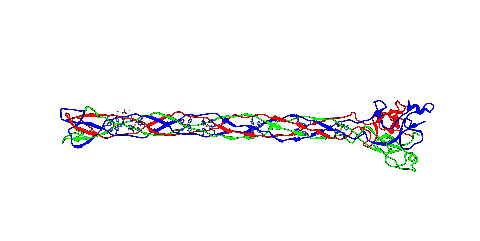
\includegraphics[width=\textwidth, trim={-10 30 -10 40}, clip]{/Users/joehealey/Documents/Warwick/PhD/Thesis/chapters/chapter5/img/2xgf.pdf}
        \captionsetup{singlelinecheck=off, justification=centering, font=footnotesize, aboveskip=10pt}
        \caption{}
    \end{subfigure}%
    
     \begin{subfigure}{\textwidth}
        \centering
        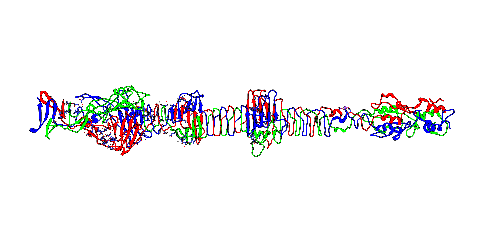
\includegraphics[width=\textwidth, trim={-10 30 -10 30 }, clip]{/Users/joehealey/Documents/Warwick/PhD/Thesis/chapters/chapter5/img/5nxf.pdf}
        \captionsetup{singlelinecheck=off, justification=centering, font=footnotesize, aboveskip=10pt}
        \caption{}
    \end{subfigure}%
    
    \begin{subfigure}{0.49\textwidth}
            \centering
            {%
            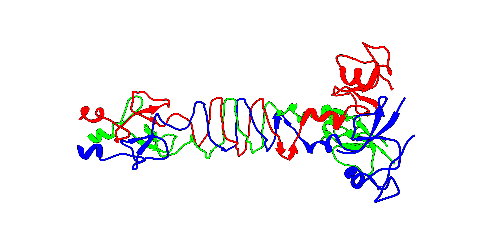
\includegraphics[width=\textwidth, trim={0 0 0 0}, clip]{/Users/joehealey/Documents/Warwick/PhD/Thesis/chapters/chapter5/img/1h6w.pdf}
            }%
            \captionsetup{singlelinecheck=off, justification=centering, font=footnotesize, aboveskip=10pt}
            \caption{}
        \end{subfigure}%
            \begin{subfigure}{0.49\textwidth}
            \centering
            {%
            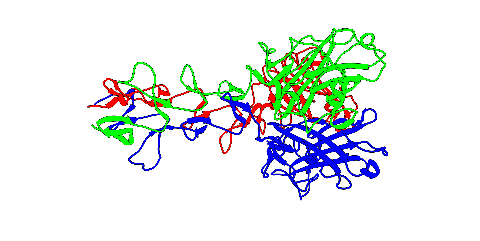
\includegraphics[width=\textwidth, trim={0 0 0 0}, clip]{/Users/joehealey/Documents/Warwick/PhD/Thesis/chapters/chapter5/img/1qiu.pdf}
            }%
            \captionsetup{singlelinecheck=off, justification=centering, font=footnotesize, aboveskip=10pt}
            \caption{}
            \label{1qiu}
        \end{subfigure}%
        
        \begin{subfigure}{0.49\textwidth}
            \centering
            {%
            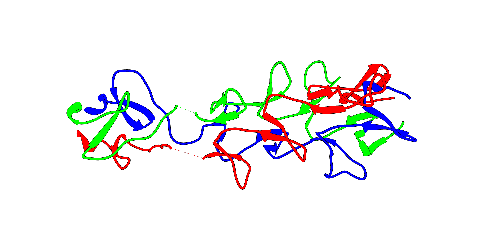
\includegraphics[width=\textwidth, trim={0 0 0 0}, clip]{/Users/joehealey/Documents/Warwick/PhD/Thesis/chapters/chapter5/img/1v1h.pdf}
            }%
           \captionsetup{singlelinecheck=off, justification=centering, font=footnotesize, aboveskip=10pt}
            \caption{}
            \label{1v1h}
        \end{subfigure}%
        \begin{subfigure}{0.49\textwidth}
            \centering
            {%
            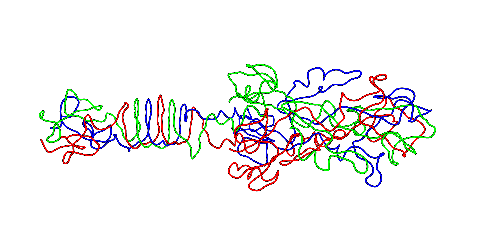
\includegraphics[width=\textwidth, trim={0 0 0 0}, clip]{/Users/joehealey/Documents/Warwick/PhD/Thesis/chapters/chapter5/img/1pdi.pdf}
            }%
           \captionsetup{singlelinecheck=off, justification=centering, font=footnotesize, aboveskip=10pt}
            \caption{}            
        \end{subfigure}%
        
	\captionsetup{singlelinecheck=off, justification=justified, font=footnotesize, aboveskip=10pt}
	\caption[Existing resolved tail fibre protein structures]{\textsc{\normalsize Crystal structures for resolved tail fibre-like proteins.}\vspace{0.1cm} \newline Reference structures for other tail fibre like structures, some of which occur in the results of HHPred homology searches for PVC13 proteins. Note in-particular, the conserved twisted trimeric nature of the structures, and the co-ordination of metal atoms in a number of the structures (denoted by the side chains being present). Structures are not scaled relative to one another. \textbf{(A)} The crystal structure of the T4 phage long fibre receptor binding tip (gp37 residues 785 to 1026) (PDB ID 2XGF), as determined in \cite{Bartual2010}. \textbf{(B)} The crystal structure of the T4 phage long fibre shaft (gp34 residues 95 to 1289) (PDB ID 5NXF), as determined in \cite{Granell2014}. \textbf{(C)} The crystal structure of the ``heat and protease resistant fragment" of the T4 phage short fibre (PDB ID 1H6W), as determined in \cite{VanRaaij2001}. \textbf{(D)} The crystal structure of the human Adenovirus C serotype 2 shaft region (PDB ID 1QIU), as determined in \cite{VanRaaij1999}. \textbf{(E)} The crystal structure of an artificial chimeric tail fibre protein, comprised of human Adenovirus C serotype 2 shaft and T4 phage fibre domains (PDB ID 1V1H), as determined in \cite{Papanikolopoulou2004}. \textbf{(F)} The crystal structure of the short tail fibre C-terminal region as fitted in to the T4 baseplate in \cite{Kostyuchenko2003} (PDB ID 1PDI). }
	\label{tailfibrestructures}
\end{figure}


It was decided to study the putative tail fibres of the PVCs further experimentally for a few reasons. Firstly, existing genome annotations and homology searches had attributed fibre-like orthology to the sequences, but typically with low confidence and low overall sequence coverage. As mentioned in previous sections, the putative PVC tail fibres had also shown a curious similarity to Adenoviral motifs, which, it appears, has not been seen in phage-like tail fibres before. Moreover, the putative fibre genes showed a great deal of variation, even between PVC operons. As explained in \vref{bioinformatics}, they are the least congruent of all the genes studied, across all the operons, and this also results in inconsistent database hits between different genes. Combined, this meant that it was unclear whether these were meaningful orthologies or merely artifactual/spurious hits; and therefore some experimental investigation would be valuable.

Though there are resolved tail fibre structures, they have been difficult to study structurally in the past. This is primarily due to them only being anchored to the main tube apparatus at one end, such that the target recognition site of the fibre at the distal end is freely mobile in order to bind the cell surface. Consequently, when averaging multiple images in electron microscopy reconstructions, the tail fibres may not consistently overlap, and are averaged out, as in the case in the \cite{Ge2015} paper for instance. In \cite{Heymann2013} (see \vref{afpstructure}), there appear to be tail fibre like structures laid back along the length of the Afp sheath in some form of docked, latent, position and this appears to have sufficiently immobilised them such that their densities can be visualised. However, this conformation appears to be an exception, rather than the rule in the structures studied to date; and though this is the most probable explanation for those densities, the map is only $\approx$20 \AA, and is thus not entirely conclusive.

Existing computational methods such as the simulations described in \vref{structbioinfo} can fail to produce plausible structures in many cases. \emph{Ab initio} methods are still difficult to implement for large multi-chain structures, as, without approximation via coarse graining, calculations simply scale too poorly due the worse-than-exponential increase in atomic interactions as a system grows in size. Not to mention, molecular dynamics is an entire field of its own, and not readily amenable to most researchers. Threading webservers such as I-Tasser \citep{Yang2014, Zhang2008, Roy2010} (used in \vref{structbioinfo}) and Phyre2 \citep{Kelly2015} have addressed this by making easy to use job submission interfaces for homology modelling. Threading approaches sometimes produce workable structures, however accuracy can become compromised for proteins with split domain structure (chimeras), where the best template protein is different for each domain, without artificially breaking the gene up and then having to `stitch together' the resultant models. Inclusion of a molecular dynamics-based refinement step, may actually worsen a simulated monomer if it's ordinarily part of a non-globular multimeric structure, by allowing the model to relax (e.g. in energy minimisation/solvation), as it will cease to be constrained to the threaded chain.

This leaves experimental structural determination as the best option, though it remains non trivial. Structural resolution via Nuclear Magnetic Resonance is unlikely to be feasible for most tail fibres. There is an upper bound on the size that NMR studies can resolve ($\approx$35 kDa), which even some of the smallest tail fibres exceed, due to their trimeric nature. It is possible that sub-cloning the proteins on a domain-by-domain basis may be within the range NMR could be applicable to, but this would become laborious and raise issues about correct folding and so on. Cryo-EM is also a possibility; as seen in the Heymann paper, it has the resolution to image the tail fibres in complex with the tail tube, but with the caveat that they are immobilised by the tube itself to prevent class averaging losing the densities. Additionally, the fibres may only be a few atoms thick at their thinnest point, which without high-end equipment could be extremely difficult to image effectively due to low contrast. This leaves X-ray crystallography as the main viable option, but this is also not without caveats. In a number of papers (such as those producing the structures in \vref{tailfibrestructures}), crystallisation was only achievable when expressing sub-cloned domains of the the protein, and often required the presence of multiple chaperones too.

The variability, above and beyond that of the rest of the operons, in the tail fibre proteins of the PVCs, combined with the PVCs known role as anti-eukaryotic effector delivery systems, suggests that their tail fibre proteins may be of particular interest. Understanding the existing target binding spectrum may elucidate the role of the PVCs in virulence and pathogenesis during \emph{Photorhabdus}' infection cycle in the various hosts it exploits. In future we would also like to be able to explore rational modification and engineering of the tail fibres, potentially controlling their tropisms. This is effectively a case of recapitulating similar studies which have been done for re-targeted R-type pyocins \citep{Scholl2009a}, whereby tail fibres were swapped or fused, conferring new target cell spectrums to pyocins that would ordinarily have no effect on the cell type of interest. In the case of the PVCs, a natural repertoire of diverse tail fibres exists, providing an as-yet-unstudied library of motifs to potentially target different cell types - though a crucial difference being that these cell types will be eukaryotic rather than prokaryotic.

In summary, this chapter examines tail fibres in isolation from the difficult-to-manipulate PVCs; in order to scrutinse their structure, orthology, and function.

\subsection*{Chapter Aims:}
\begin{itemize}
	\item Clone and express tagged versions of putative tail-fibres from different PVC operons.
	\item Devise and optimise a purification strategy.
	\item Probe tail fibre structure via biochemical/biophysical/crystallographic methods.
	\item Exploit functionalised tail-fibre complexes for binding studies.
\end{itemize}
\clearpage

\section{Experimental Procedures}

\subsection{\emph{in silico} Profiling of Tail Fibre Sequences}
The putative tail fibre hereafter called `pnf13' was cloned from the \Pasy{} ATCC43949 (a.k.a. ``USA'') PVC-pnf operon; similarly, the putative tail fibre `lumt13' was cloned from the PVC-lumt operon of the same genome. They both carry the designation `13' from their general syntenic position within the operon, however the lumt operon does have an upstream deletion. Operon organisation is covered in previous chapters, but \vref{pnflocus} and \vref{lumtlocus} show the fibres in their genomic/gene cluster context.

\vspace{0.1cm}
\begin{figure}[h]
	\centering
	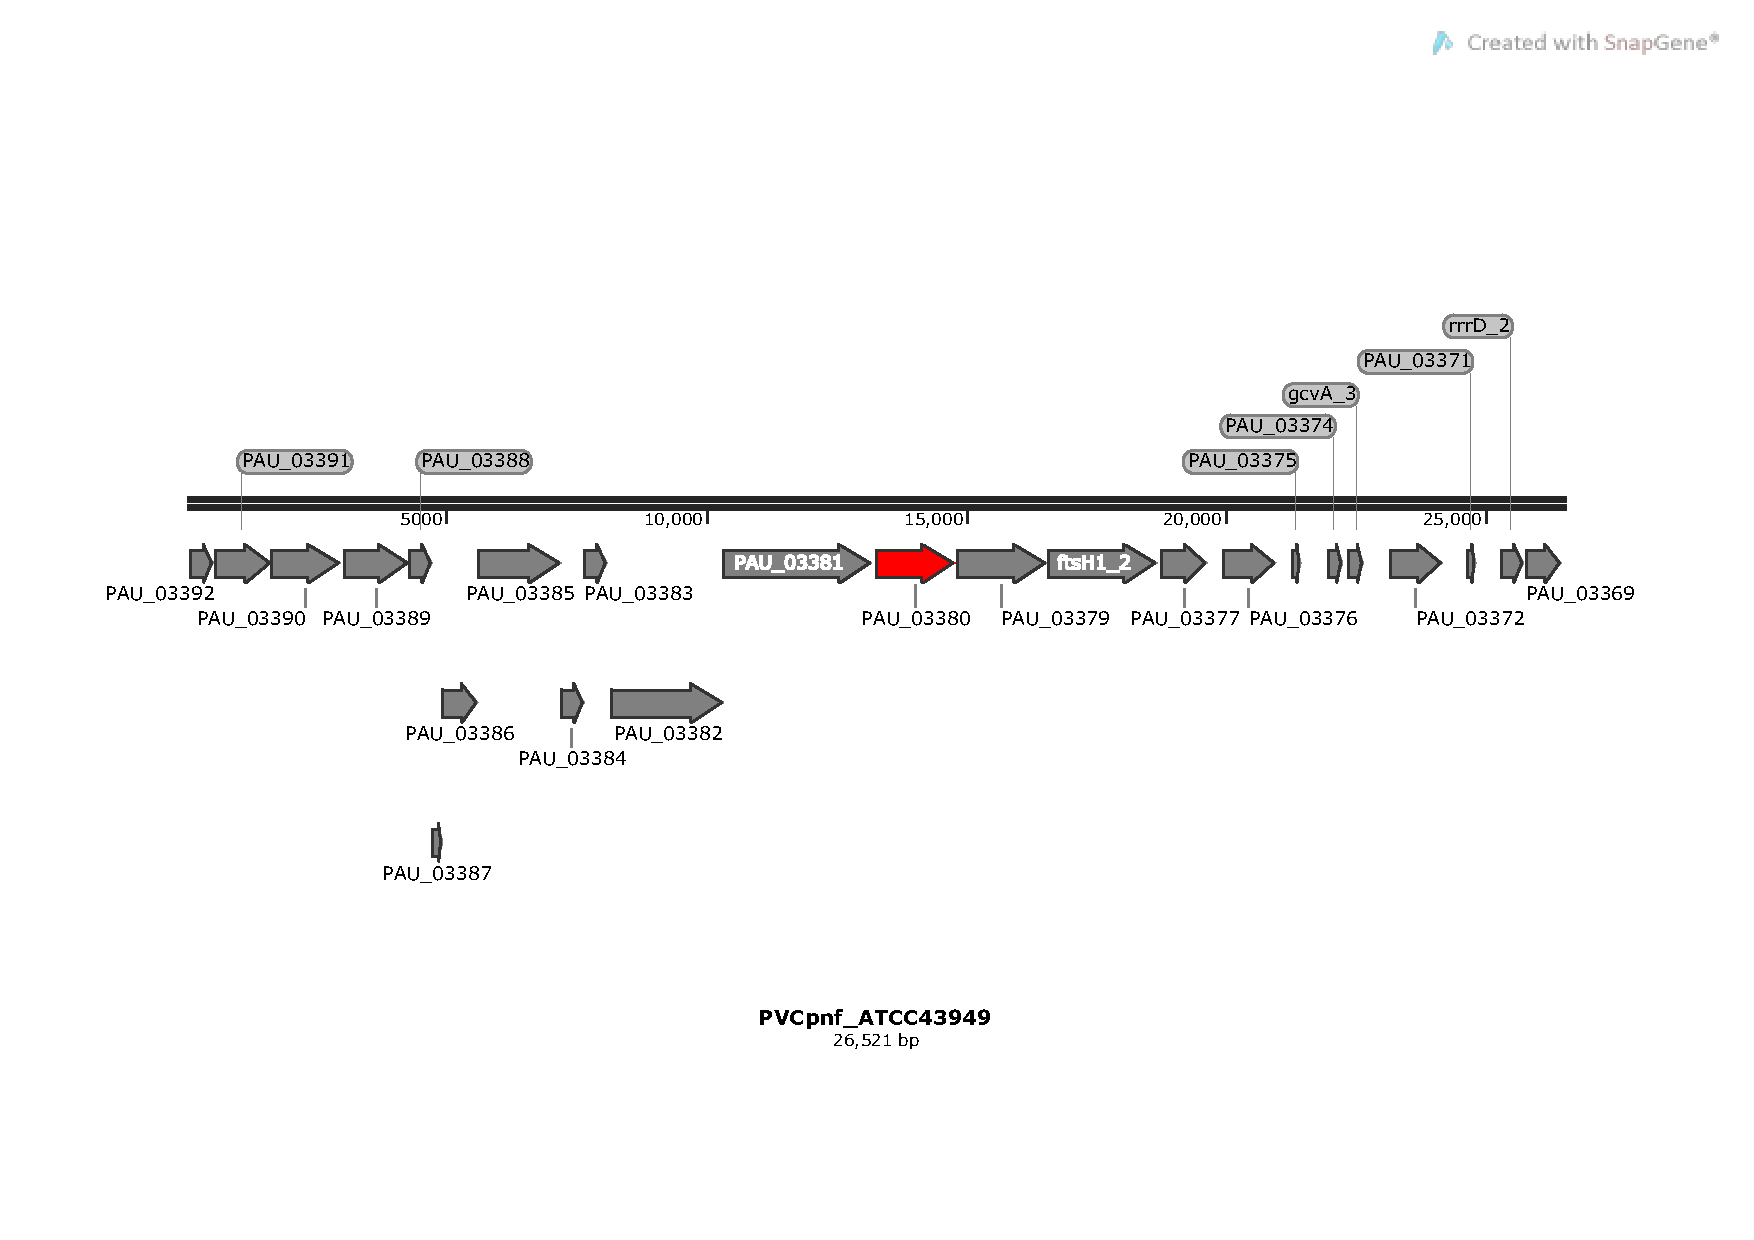
\includegraphics[width=\textwidth, trim={50, 220, 55, 150}, clip]{/Users/joehealey/Documents/Warwick/PhD/Thesis/chapters/chapter5/img/PVCpnf_ATCC43949_Map.pdf}
	\captionsetup{singlelinecheck=off, justification=justified, font=footnotesize, aboveskip=5pt}
	\caption[PVCpnf operon map identifying cloned PVCpnf13 protein]{\textsc{\normalsize The ``pnf" operon from \emph{P. asymbiotica} ATCC43949.}\vspace{0.1cm} \newline The PVC\emph{pnf} operon, with the putative tail fibre gene (PVCpnf13) that was cloned in red. Locus tags correspond to the most recent genome annotation used throughout this study.}
	\label{pnflocus}
\end{figure}
\vspace{-0.7cm}
\begin{figure}[h]
	\centering
	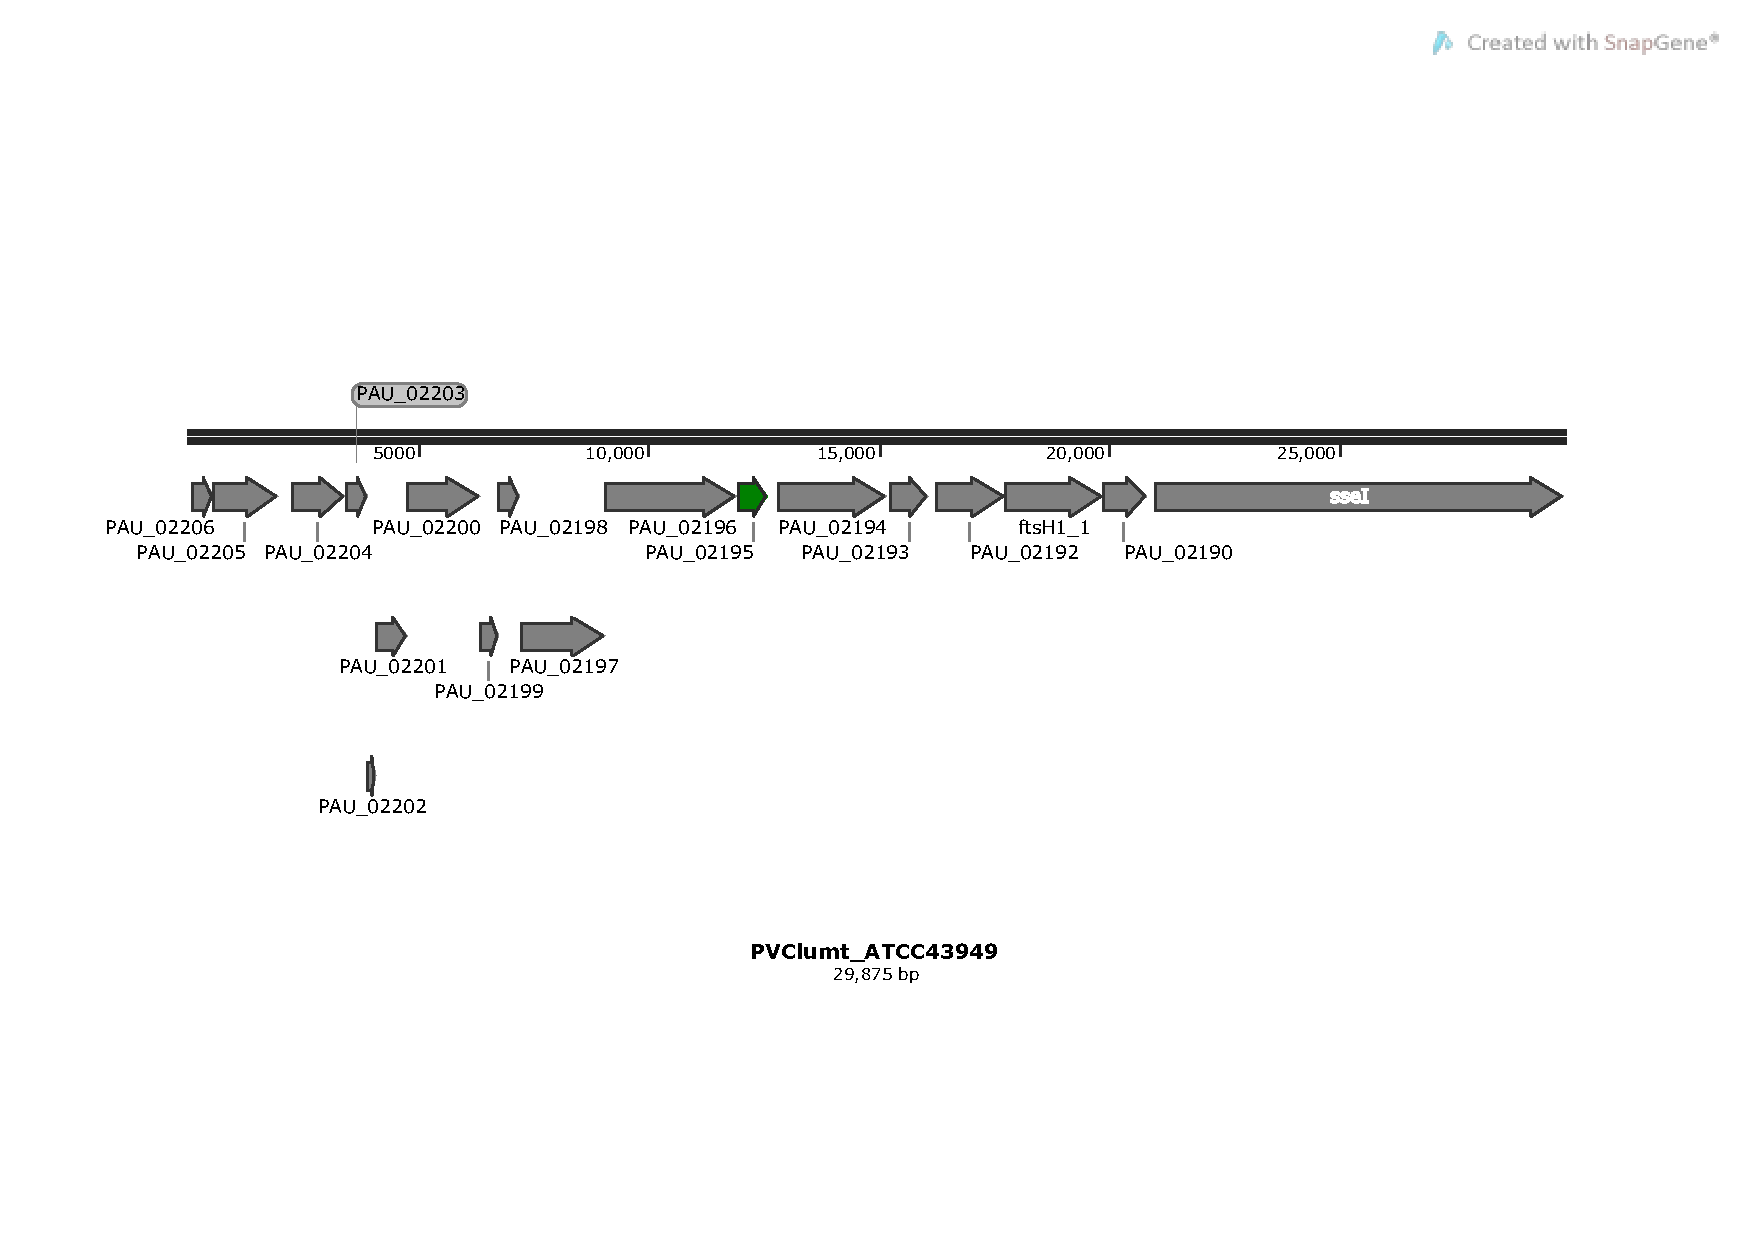
\includegraphics[width=\textwidth, trim={50, 200, 55, 150}, clip]{/Users/joehealey/Documents/Warwick/PhD/Thesis/chapters/chapter5/img/PVClumt_ATCC43949_Map.pdf}
	\captionsetup{singlelinecheck=off, justification=justified, font=footnotesize, aboveskip=10pt}
	\caption[PVClumt operon map identifying cloned PVClumt13 protein]{\textsc{\normalsize The ``lumt" operon from \emph{P. asymbiotica} ATCC43949.}\vspace{0.1cm} \newline The PVC\emph{lumt} operon, with the putative tail fibre gene (PVClumt13) that was cloned in green. Locus tags correspond to the most recent genome annotation used throughout this study.}
	\label{lumtlocus}
\end{figure}

These two particular tail-fibres were chosen from the many choices as they are both unique to the human pathogenic strains but from disparate operons, and would allow us to explore differential tissue culture activities etc. Though the operons group together in \vref{consensustree}, it can be seen from Figure \ref{pnflocus} and \vref{lumtlocus} that the two genes, despite having putatively the same function, are significantly different sizes and therefore could have quite different higher order structure. In the case of \emph{lumt13}, the CDS encodes a 23.6 kDa protein (as a monomer), and \emph{pnf13} is twice as large at 51.7 kDa. This is suggestive, therefore, of two tail fibres which are both evolved to act against eukaryotic targets, but potentially with each honed in a different manner, to exploit different molecular mechanisms.

\subsubsection{Domain Structure}\label{domainstructuresection}
Probably the most interesting aspect of these two proteins (and tail fibres from PVC operons in general) is their apparent chimerism in domain structure as demonstrated in the HHPred results from \vref{hhresults}. \vref{domainstructure} summarises the HHPred hits for these two tail fibres. They match distinct PDB entries in different regions, typically from either T4 bacteriophages or human Adenovirus fibre proteins.

This is suggestive of \Pa{} perhaps co-opting Adenoviral motifs (or something at least resembling Adenovirus motifs) in the environment or perhaps during infection of mammalian systems. PVCpnf and PVClumt are unique to the mammalian pathogenic strains providing both `motive' and opportunity for recombination with a mammalian virus to have occurred. However, this is also true of some \emph{P. luminescens} operons too, and thus may point to an ancestor that was capable of mammalian infection, and that \emph{P. luminescens} has subsequently lost this capability. An alternative suggestion is simply convergent evolution, and both Adenoviruses and PVC fibres have evolved to a specific receptor or receptor family. Some evidence for this can be taken from the fact that both Coxsackie and Adenoviruses bind to the so-called ``CAR'' or ``Coxsackie and Adenovirus Receptor", despite both being evolutionarily disparate viruses (the former is a (+)ssRNA virus (Group IV) and the latter a dsDNA (Group I) virus). Since these two distinct viruses have both evolved to exploit the same receptor, it is not a big leap to suppose that PVCs may also have done so.

Since the PVCs themselves are similar in structure to T4 phage tails, it is likely that the split domain structure maintaining a T4 region is required for `mounting' the fibre on to the sheath complex. This implicitly suggests two points; firstly that the tail fibres do need to maintain a phage like domain within the protein, albeit somewhat diversified, to enable `mounting' to the tube of the PVC, much as T4 fibres would need to mount to the tail tube of the phage. However, the homologies are lower in comparison which would suggest that the PVC tail fibres and the tube itself may be drifting together to become more `bespoke'. There is an additional subtlety to consider; the protein structure databases are rich in T4 and Adenovirus structures, to the point of bias, so it is small wonder that they match these structures when searched. But, if the suggestions of \cite{Sarris2014} are to be believed, PVCs and other tail-tube like elements may have diverged in deep time, in which case their tail fibres may be fairly unique, perhaps representing a convergently evolved structure, rather than a chance recombinant one.


\footnotesize
\captionsetup{singlelinecheck=off, justification=justified, font=footnotesize}
\rowcolors{1}{gray!20}{white}
\begin{tabularx}{\textwidth}{l l p{0.8cm} p{1.15cm} p{1.15cm} p{0.8cm} >{\setlength{\baselineskip}{0.9\baselineskip}}m{0.465\textwidth}}
\hiderowcolors
\caption[Cloned tail fibre domains according to HHPred]{\textsc{\normalsize The top 5 HHPred structural homologies detected for pnf13 and lumt13.}\vspace{0.1cm}}
\label{domainstructure}\\

\# & PDB Hit & Prob & E-Value & P-Value & Score & Hit Descriptor\\[0.5ex]
\hline\hline
\multicolumn{7}{p{\linewidth}}{\centering pnf13 (PAU\_03380)}\tstrut\bstrut \\
\hline
\showrowcolors
1 & 3IZO\ & 98.1 & \sn{2.8}{-9} & \sn{7.3}{-14} & 107.6 & Fiber; pentameric penton base, trimeric viral protein; 3.60 \AA \{Human Adenovirus 5\} \\
2 & 3IZO & 97.6 & \sn{1.3}{-7}  & \sn{3.4}{-12} & 95.6 & Fiber; pentameric penton base, trimeric viral protein; 3.60 \AA \{Human Adenovirus 5\} \\
3 & 1OCY & 97.6 & \sn{1.8}{-7}  & \sn{4.7}{-12} & 80.4 & Bacteriophage T4 short tail fibre; 1.5 \AA \{Bacteriophage T4\}\\
4 & 1V1H & 96.1 & 0.00012       & \sn{3}{-9}  &   60.4 & Fibritin, fiber protein; chimera; 1.9 \AA \{Human Adenovirus type 2\} \\
5 & 1V1H & 95.9 & 0.0002        & \sn{5.1}{-9}  &   59.1 & Fibritin, fiber protein; chimera; 1.9 \AA \{Human Adenovirus type 2\} \\
\hiderowcolors\hline
\multicolumn{7}{p{\linewidth}}{\centering lumt13 (PAU\_02195)}\tstrut\bstrut \\
\hline
\showrowcolors
1 & 1V1H & 97.7 & \sn{9.4}{-8} & \sn{2.4}{-12} & 71.3 & Fibritin, fiber protein; chimera; 1.9 \AA \{Human Adenovirus type 2\} \\
2 & 1V1H & 96.3 & \sn{5.9}{-5} & \sn{1.5}{-9} & 56.3 & Fibritin, fiber protein; chimera; 1.9 \AA \{Human Adenovirus type 2\}\\
3 & 1QIU & 95.8 & 0.00028      & \sn{7.2}{-9} & 60.4 & Adenovirus fibre; fibre protein, triple beta-spiral; 2.4 \AA \{Human Adenovirus 2\}\\
4 & 3IZO & 94.7 & 0.0025       & \sn{6.4}{-8} & 59.1 & Fiber; pentameric penton base, trimeric viral protein; 3.60 \AA \{Human Adenovirus 5\} \\
5 & 1OCY & 66.7 & 1.3          & \sn{5.3}{-7} & 33.1 & Bacteriophage T4 short tail fibre; structural protein, 1.5 \AA \{Bacteriophage T4\} \\
\hline
\end{tabularx}
\normalsize

\begin{figure}[h]
	\centering
	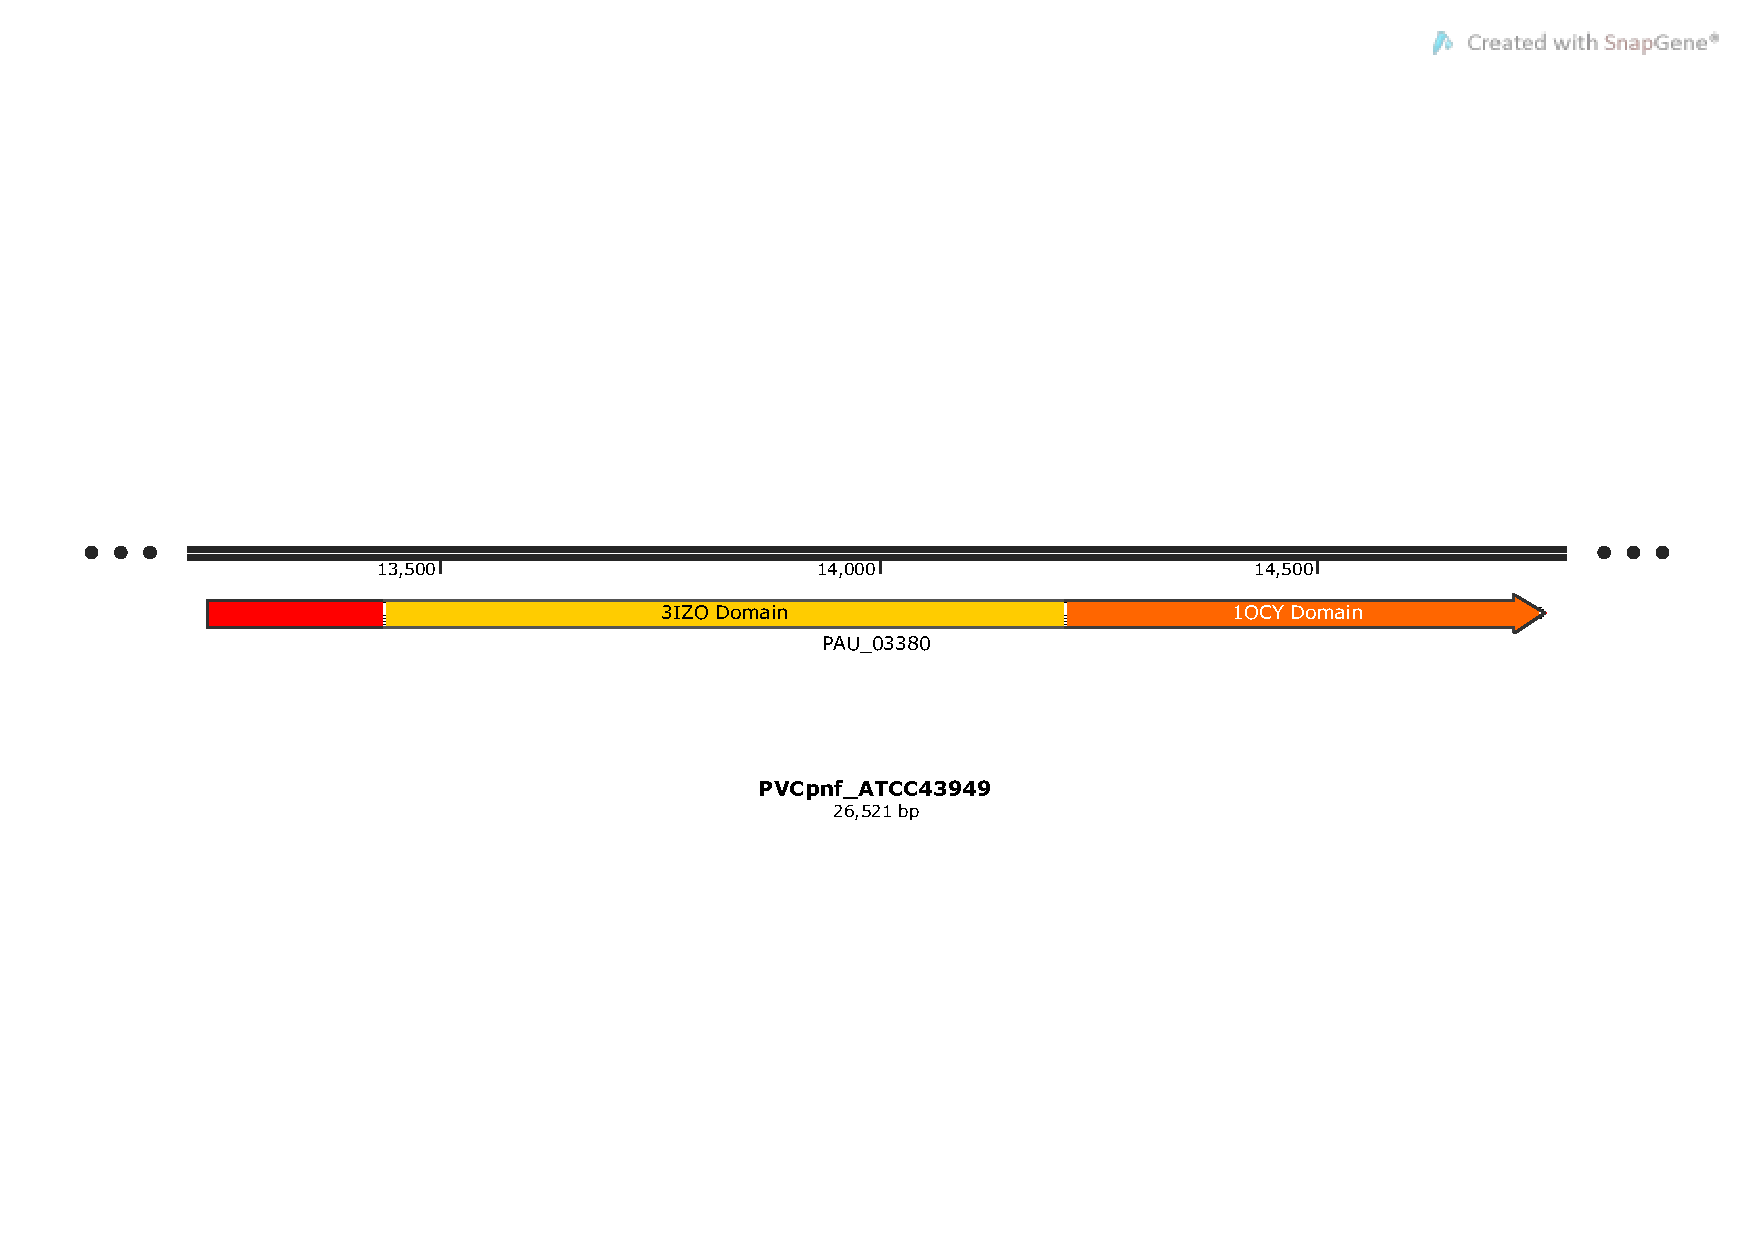
\includegraphics[width=\textwidth, trim={50, 250, 55, 250}, clip]{/Users/joehealey/Documents/Warwick/PhD/Thesis/chapters/chapter5/img/pnf13_domain_map.pdf}
	\captionsetup{singlelinecheck=off, justification=justified, font=footnotesize, aboveskip=0pt}
	\caption[The domain structure of the PVCpnf13 tail fibre protein]{\textsc{\normalsize The PVCpnf13 tail fibre with dominant domain homologies depicted}\vspace{0.1cm} \newline A map of the dominant protein domain splits within the PVCpnf13 tail fibre protein according to HHPred. Toward the 3' end there is a region which matches well to the PDB ID 3IZO, a fibre protein-penton base from the human Adenovirus 5, as determined in \cite{Liu2011}. At the 5' end, a domain match to the Bacteriophage T4 short tail fibre (PDB ID 1OCY , as determined in \cite{Thomassen2003}) can be seen. The protein therefore resembles a natural chimera/fusion protein of an Adenoviral motif and a phage motif. Interestingly, PVCpnf13 also shares similarities to PDB ID 1V1H, which is an artificial Adenovirus-phage fibre chimera, created in the study by \cite{Papanikolopoulou2004}.}
	\label{pnfdomains}
	\end{figure}
\begin{figure}[h]
	\centering
	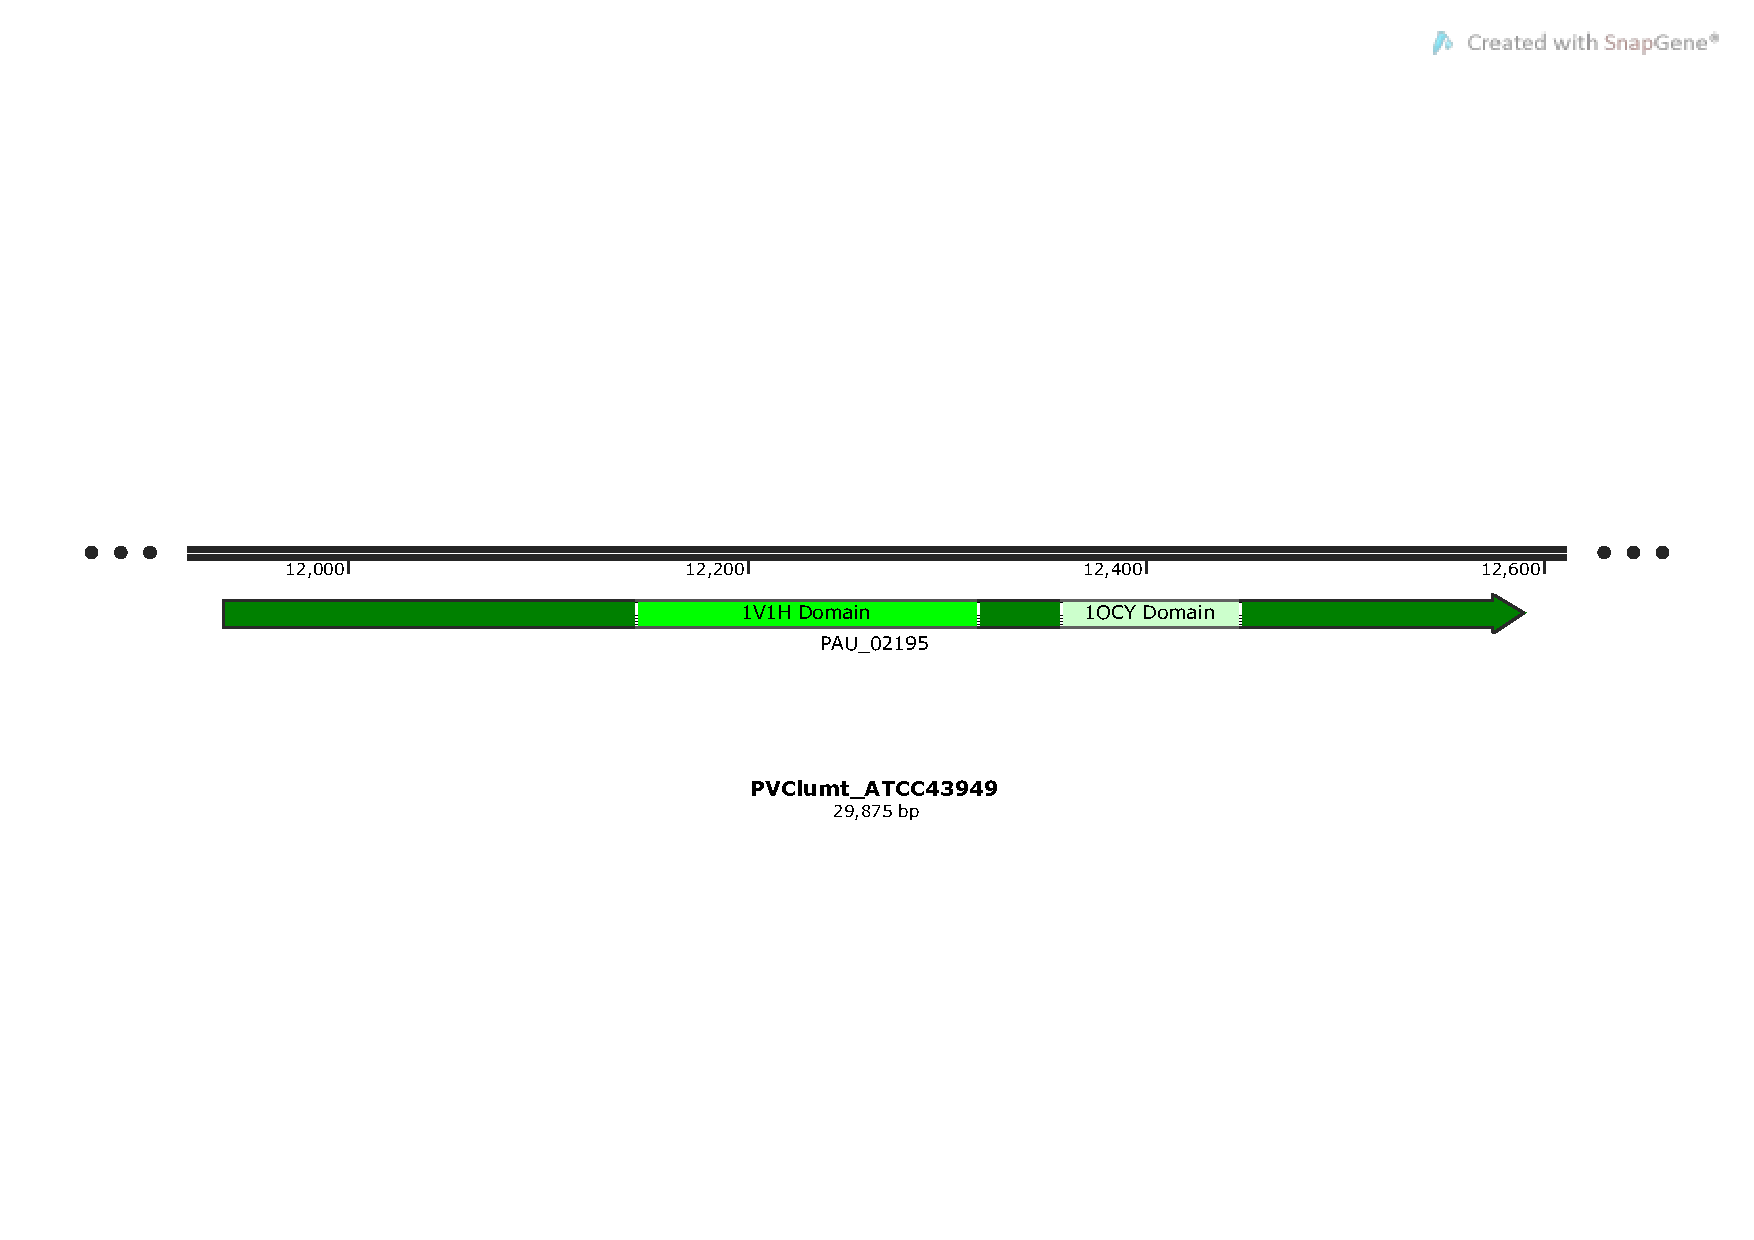
\includegraphics[width=\textwidth, trim={50, 250, 55, 250}, clip]{/Users/joehealey/Documents/Warwick/PhD/Thesis/chapters/chapter5/img/lumt13_domain_map.pdf}
	\captionsetup{singlelinecheck=off, justification=justified, font=footnotesize, aboveskip=0pt}
	\caption[The domain structure of the PVClumt13 tail fibre protein]{\textsc{\normalsize The PVClumt13 tail fibre with dominant domain homologies depicted}\vspace{0.1cm} \newline A map of the dominant protein domain splits within the PVClumt13 tail fibre protein according to HHPred. Toward the 3' end there is a region which matches to the PDB ID 1V1H, an artificial fibre fusion protein from the human Adenovirus 5 and the T4 phage \cite{Papanikolopoulou2004}. At the 5' end, a domain match to the Bacteriophage T4 short tail fibre (PDB ID 1OCY, as determined in \cite{Thomassen2003}) can be seen. The protein therefore resembles a natural chimera/fusion protein of an Adenoviral motif and a phage motif.}
	\label{lumtdomains}
\end{figure}



\subsubsection{Sequence Characteristics}
As well as identifying the orthologues of the sequences using HMMs like those in \vref{domainstructure}, a hallmark of putative tail fibre sequences is the coordination of metal atoms, like those seen in several of the structures in \vref{tailfibrestructures}. For example, in the tail fibre tip structure PDB ID 2XGF solved by \cite{Bartual2010}, it was observed that iron was present in the crystal structures, most likely in the Fe$^{2+}$ oxidation state. They were able to identify seven iron sites within the crystal, and this matched the frequent occurrence of His-$x$-His motifs within the protein sequence. The authors were also able to obtain improved stability of expressed proteins when supplementing growth media with Manganese (II) chloride, and though they did not identify any Manganese in the final crystals/structures, they concluded that this is indicative of the need for metal ions in a 2+ oxidation state. Continuing the theme, in \cite{VanRaaij2001}, they were able to identify a set of conserved repeats, in the receptor binding tip of the T4 short tail fibre. To examine if a similar sequence pattern might be evident in the PVC tail fibres, sequences were analysed with the Rapid Automatic Detection and Alignment of Repeats program from the EMBL \citep{Heger2000}. For the two proteins being studied here, the results are displayed in \vrefrange{pnfrepeats}{lumtrepeats}. Repeats are identifiable in all but one of the tail fibre proteins, and typically runs of four to six repeats can be detected to varying degrees of sequence identity. PVCpnf is unusually repetitive, even among the tail fibres, with 10 very conserved repeat patterns, each separated by two amino acids (see \vref{pnfrepeats}). The next most repetitive proteins are PLT\_01746, the tail fibre from the \emph{P. luminescens} TT01 ``Unit 1" operon, and PAK\_02618, from the \emph{P. asymbiotica} Kingscliff ``Unit 1" operon, both of which have 7 tandem repeats (note: these two operons are not orthologues, despite the naming scheme). Given the likely role of the repeats in forming the shaft region of the phage fibres, this suggests that the pnf tail fibre should be, potentially substantially, longer than the lumt one\footnote{Data for other tail fibres not shown}. The significance that this might have is not yet understood however. Interestingly, in the recent paper by \cite{Hurst2018}, the tail fibres of the newly identified AfpX demonstrated a tail fibre repeat architecture very similar to that of the PVCpnf13, with an even greater number of tandem 15-residue repeats, that were also quite rich in valine, serine and glycine. Since the tail fibres which are seen in the EM density map in \vref{afp1} appear to be very long (substantially longer than some very preliminary EM densities obtained for a PVC via collaboration with the Max Planck institute at Dortmund (data not shown)), it makes sense that the sequences for the PVC tail fibres contain fewer repeats and thus potentially shorter shaft regions.

Belying their diversity, there does not appear to be one particular structural motif across all the tail fibre proteins - there are no motifs such as the T4 fibre's H-$x$-H which seems to predominate any particular fibre. In the multiple sequence alignment which has been reproduced from the Appendices in \vref{tailfibremsa}. It is possible to identify 4 seemingly conserved domains, but there appears to be no obvious conservation of repeats, despite (nearly) all of the tail fibre proteins having repetitive stretches. 

\clearpage

\footnotesize
\captionsetup{singlelinecheck=off, justification=justified, font=footnotesize}
\rowcolors{1}{gray!20}{white}
\begin{tabularx}{\textwidth}{ >{\raggedright\arraybackslash} m{0.20\textwidth} >{\raggedright\arraybackslash} m{0.24\textwidth} Z l l l l l}
\hiderowcolors
\caption[Sequence repeats detected in the PVCpnf13 tail fibre]{\textsc{\normalsize The largest stretches of sequence repeats within the PVCpnf13 tail fibre.} \vspace{0.1cm} \newline This table shows the sequences and statistics for the repeat detection from RADAR, for PVCpnf13. A well conserved set of 10, 14 amino acid stretches can be found, which are rich in valines, lysines, serines and glycines, and each 15 amino acid stretch is separated by 2 amino acids.}
\label{pnfrepeats}\\

\# Repeats & Total Score & Length  & Diagonal & BW-From & BW-To & Level\\[0.5ex]
\hline\hline
  10  &     298.40  &      15  &      15  &     200  &     214  &       1 \\
  \hline
  & & & & & & & \\[-2.5ex]
  \hline
 Repeat Indices & Alignment Score/Z-score &\multicolumn{6}{l}{\texttt{Repeat Sequence}} \\
\showrowcolors
 \hline\hline
  149 - 163 & (25.32/10.54) & \multicolumn{6}{l}{\texttt{VKVSANKGLSVDSSG}} \\
  166 - 180 & (29.64/13.67)  & \multicolumn{6}{l}{\texttt{VKVNTDKGISVDGNG}} \\
  183 - 197 & (29.67/13.68) & \multicolumn{6}{l}{\texttt{VKVNTSKGISVDNTG}} \\
  200 - 214 & (31.92/15.31) & \multicolumn{6}{l}{\texttt{VIANASKGISVDGSG}} \\
  217 - 231 & (33.00/16.10) & \multicolumn{6}{l}{\texttt{VIANTSKGISVDGSG}} \\
  234 - 248 & (30.39/14.21) & \multicolumn{6}{l}{\texttt{VIANTSKGISVDNTG}} \\
  251 - 265 & (31.92/15.31) & \multicolumn{6}{l}{\texttt{VIANASKGISVDGSG}} \\
  268 - 282 & (33.00/16.10) & \multicolumn{6}{l}{\texttt{VIANTSKGISVDGSG}} \\
  285 - 299 & (31.82/15.24) & \multicolumn{6}{l}{\texttt{VIANTSKGISVDSSG}} \\
  302 - 316 & (21.72/ 7.93) & \multicolumn{6}{l}{\texttt{VKVKANGGIKVDANG}} \\

\hline

\end{tabularx}

\normalsize
\footnotesize
\captionsetup{singlelinecheck=off, justification=justified, font=footnotesize}
\rowcolors{1}{gray!20}{white}
\begin{tabularx}{\textwidth}{ >{\raggedright\arraybackslash} m{0.20\textwidth} >{\raggedright\arraybackslash} m{0.24\textwidth} Z l l l l l}
\hiderowcolors
\caption[Sequence repeats detected in the PVCpnf13 tail fibre]{\textsc{\normalsize The largest stretches of sequence repeats within the PVClumt13 tail fibre.} \vspace{0.1cm} \newline This table shows the sequences and statistics for the repeat detection from RADAR, for PVClumt13. lumt is a shorter protein, thus less propensity for long tandem repeats is possible, but 3 stretches relatively abundant in valine, isoleucine, glycine and aspartic acid are found.}
\label{lumtrepeats}\\

\# Repeats & Total Score & Length  & Diagonal & BW-From & BW-To & Level\\[0.5ex]
\hline\hline
  3&      72.06&      14&      28&      81&      94&       1 \\
  \hline
  & & & & & & & \\[-2.5ex]
  \hline
 Repeat Indices & Alignment Score/Z-score &\multicolumn{6}{l}{\texttt{Repeat Sequence}} \\
\showrowcolors
 \hline\hline
  81 - 94 & (22.51/10.89) & \multicolumn{6}{l}{\texttt{LQVKAGAGVDIDNN}} \\
  97 - 110 & (24.55/12.40)  & \multicolumn{6}{l}{\texttt{ITIKSGHGIKVDGN}} \\
  112 - 125 & (24.99/12.73) & \multicolumn{6}{l}{\texttt{ISVKPGSGIKVDSN}} \\

\hline

\end{tabularx}
\normalsize


\begin{figure}[p]
\thisfloatpagestyle{IHA-fancy-style}

\vspace{-1cm}
\begin{texshade}{/Users/joehealey/Documents/Warwick/PhD/Thesis/appendices/bioinformatics_appendix/resources/alignments/fixed_awked_PVC13_homologs.fasta}
\seqtype{P}
\setfont{numbering}{tt}{md}{sc}{tiny}
\setfont{names}{tt}{md}{up}{tiny}
\setfont{residues}{tt}{md}{sc}{tiny}
\setfont{ruler}{tt}{bf}{sc}{tiny}

\shadingmode[allmatchspecial]{similar}
\smallblockskip
\hideruler
\vsepspace{0.2pt}
\hideconsensus
\topspace{-3.5pt}
\featuresfootnotesize
\feature{top}{3}{18..83}{brace}{Conserved Domain 1}
\feature{top}{1}{83..86}{brace}{Conserved Domain 2}
\feature{top}{1}{98..102}{brace}{Conserved Domain 3}
\feature{top}{1}{115..122}{brace}{Conserved Domain 4}
\feature{top}{1}{220..250}{brace}{Hypervariable Receptor Domain}
%
%\shortcaption{Multiple sequence alignment of PVC tail fibre genes, denoting conserved domains}
%\showcaption[bottom]{\small Multiple sequence alignments for all tail fibre sequences known for the PVCs. This is the same alignment as that referred to in previous chapters and in Appendix \vref{bioinformatics_appendix}. The MSA was generated with Clustal Omega, and has been visualised here via the \texttt{TexShade} package. Residues are colour coded by residue similarity.}
%
\end{texshade}
	\captionsetup{singlelinecheck=off, justification=justified, font=footnotesize, aboveskip=2pt}
	\caption[Multiple Sequence Alignment of PVC Tail fibres]{\textsc{\normalsize Annotated multiple sequence alignment for putative PVC tail fibres}\vspace{0.1cm}\newline Alignment reproduced from Appendix \vref{bioinformatics_appendix}. Residues are colour coded by residue similarity, and identifiable domains of interest are annotated.}
	\label{tailfibremsa}
\end{figure}
\clearpage



\subsubsection{``\emph{in silico} Cloning"}

Even with the hypervariable sequence identified and some promising 3D models, it was not possible to tell categorically where the region of the tail fibres responsible for binding to the host would be in the final folded protein. It was decided to clone both of the fibres studied C- and N- terminally hexahistidine tagged in case one tag was found to interfere with the protein downstream. Primers were designed to insert the two genes in-frame with the histidine tags in pET15b (N-terminal) and pET29a (C-terminal), yielding pET15b-pnf13, pET15b-lumt13, pET29a-pnf13 and pET29a-lumt13 (see \vref{customplasmids} and \vref{methods} for technical detail such as primer sequences etc.). For each gene, the same forward primer bearing an NdeI restriction site was used for both pET15b and pET29a, with the ATG of the restriction site serving as the start codon for the gene. Reverse primers had to be redesigned for each vector, utilising a BamHI site for pET15b, and a KpnI site for pET29a. Also for pET29a, 2 additional bases were added to the histidine tag linker region to bring the tag in-frame. Construct maps can be found in \vrefrange{tailfibreplasmidspnf}{tailfibreplasmidslumt}.


\begin{figure}[p]
\thisfloatpagestyle{IHA-fancy-style}

\centering
    \begin{subfigure}{\textwidth}
        \centering
        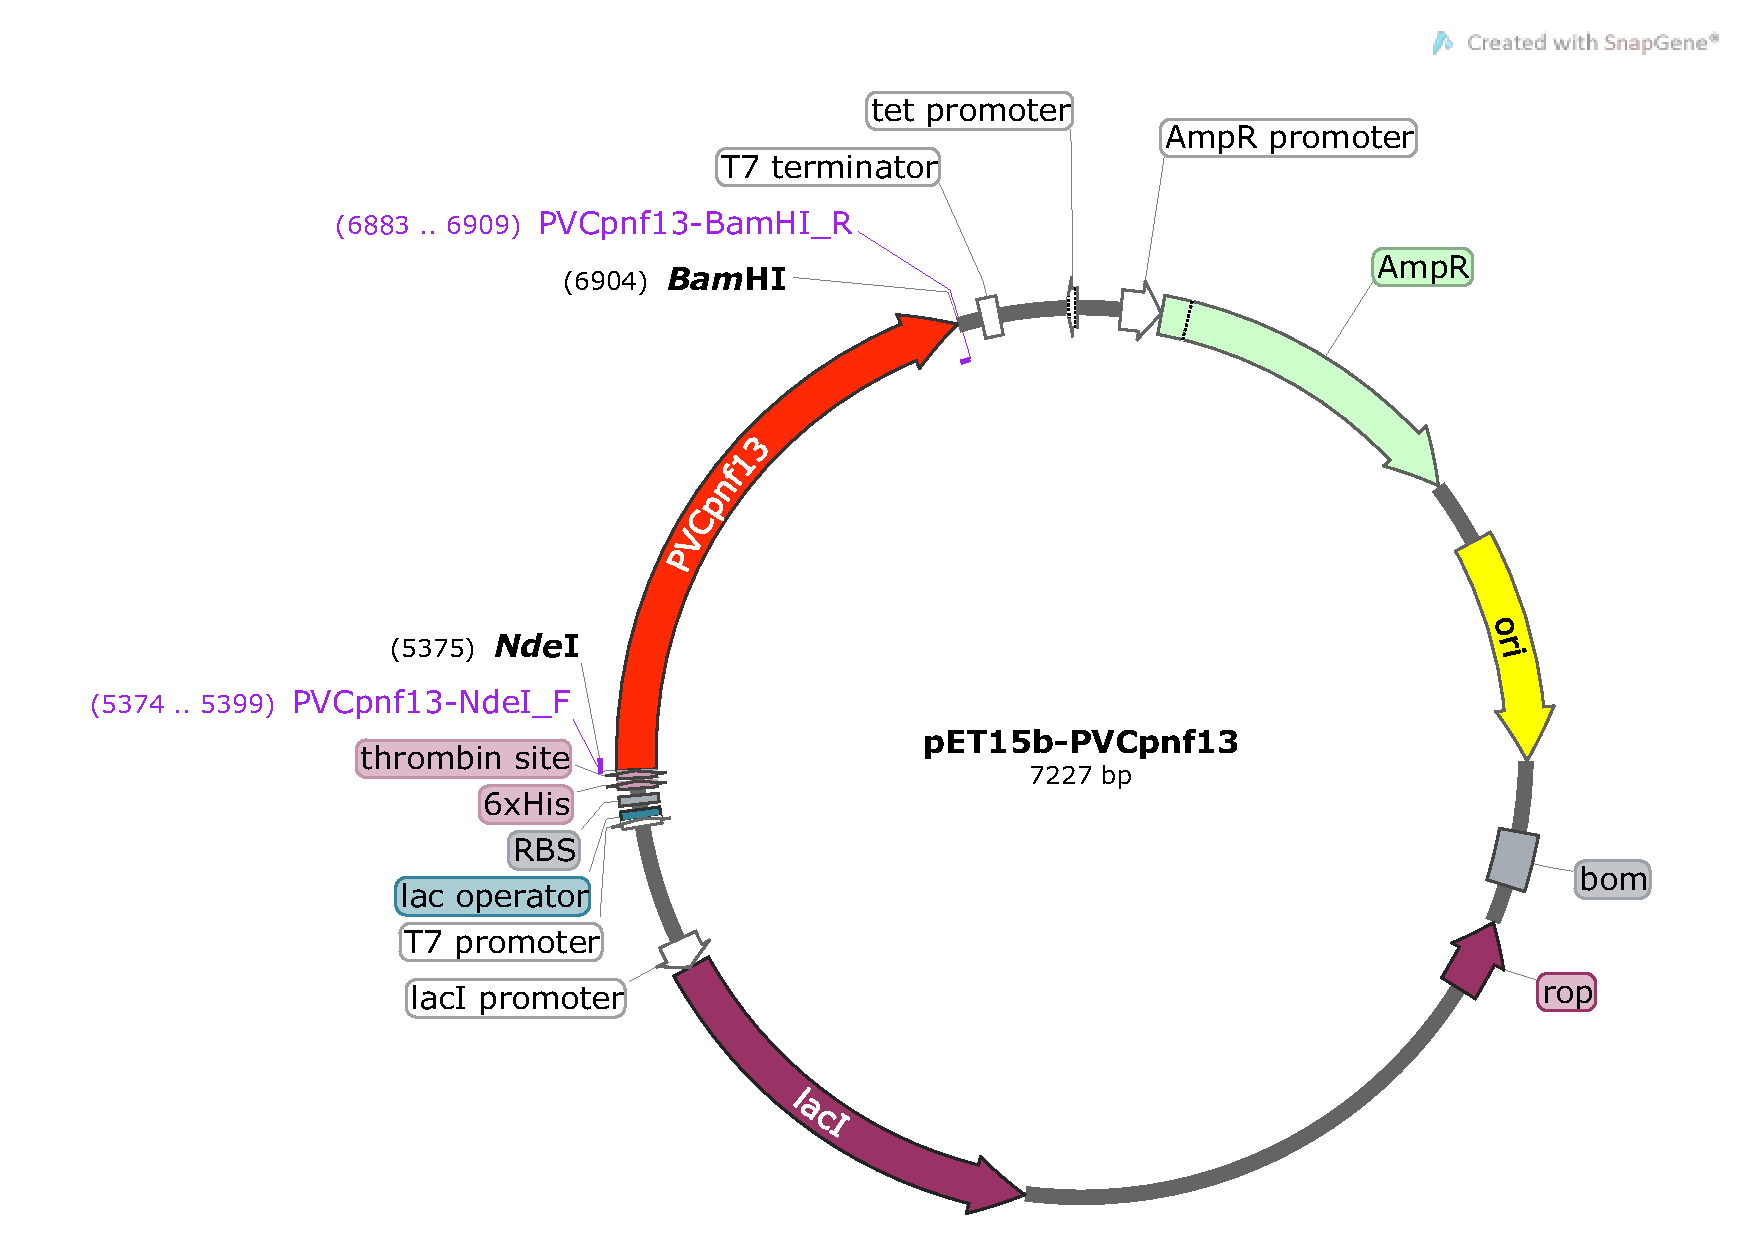
\includegraphics[width=0.85\textwidth, trim={0 0 0 40 }, clip]{/Users/joehealey/Documents/Warwick/PhD/Thesis/chapters/chapter5/img/pET15b-PVCpnf13_Map.pdf}
        \captionsetup{singlelinecheck=off, justification=centering, font=footnotesize, aboveskip=10pt}
        \caption{}
        \label{pET15pnf}
    \end{subfigure}%
    
    \vspace{0.5cm}
    
    \begin{subfigure}{\textwidth}
        \centering
            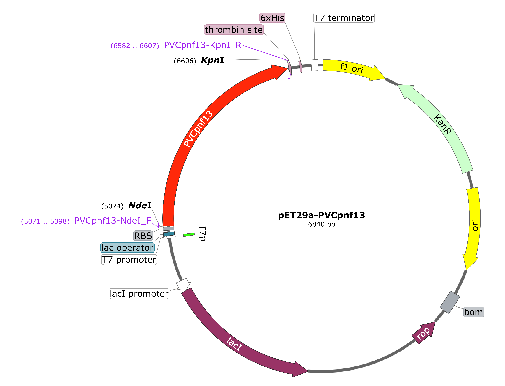
\includegraphics[width=0.85\textwidth, trim={0 0 0 40}, clip]{/Users/joehealey/Documents/Warwick/PhD/Thesis/chapters/chapter5/img/pET29a-PVCpnf13_Map.pdf}
            \captionsetup{singlelinecheck=off, justification=centering, font=footnotesize, aboveskip=10pt}
            \caption{}
            \label{pET29pnf}
        \end{subfigure}%    
	\captionsetup{singlelinecheck=off, justification=justified, font=footnotesize, aboveskip=10pt}
	\caption[Plasmid maps for cloned PVCpnf tail fibre proteins]{\textsc{\normalsize Fusion construct maps for tagged PVCpnf13 tail fibres.}\vspace{0.1cm} \newline Plasmid maps for the tail fibre-hexahistidine tag fusion proteins of the PVCpnf operon from \emph{P. asymbiotica} ATCC43949, used in this study for purification and functionalisation. The insert sequences are annotated as red CDSs, the primers are labelled in pink, restriction sites in black, fusion tags in light pink oval boxes. \textbf{(A)} The tail fibre from the PVCpnf operon fused N-terminally to a hexahistidine tag in the vector pET15b. \textbf{(B)} The tail fibre from the PVCpnf operon fused C-terminally to a hexahistidine tag in the vector pET29a.}
	\label{tailfibreplasmidspnf}
\end{figure}


\begin{figure}[p]
\thisfloatpagestyle{IHA-fancy-style}

\centering
    \begin{subfigure}{\textwidth}
        \centering
        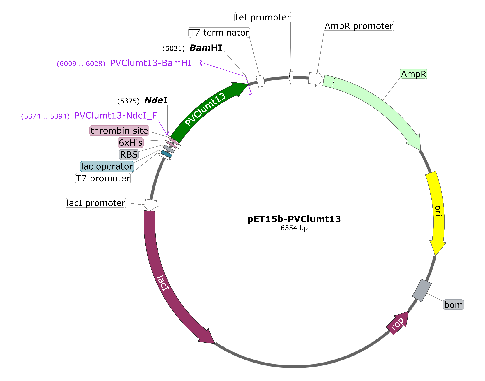
\includegraphics[width=0.85\textwidth, trim={0 0 0 40 }, clip]{/Users/joehealey/Documents/Warwick/PhD/Thesis/chapters/chapter5/img/pET15b-PVClumt13_Map.pdf}
        \captionsetup{singlelinecheck=off, justification=centering, font=footnotesize, aboveskip=10pt}
        \caption{}
        \label{pET15lumt}
    \end{subfigure}%
    
    \vspace{0.5cm}
    
    \begin{subfigure}{\textwidth}
        \centering
            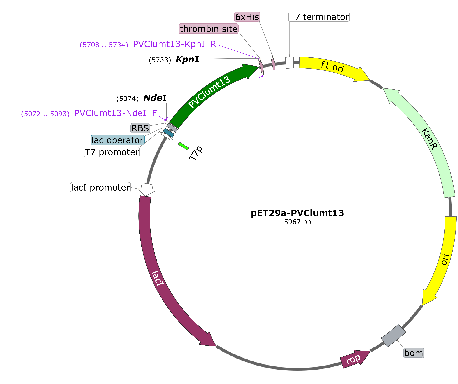
\includegraphics[width=0.85\textwidth, trim={0 0 0 40}, clip]{/Users/joehealey/Documents/Warwick/PhD/Thesis/chapters/chapter5/img/pET29a-PVClumt13_Map.pdf}
            \captionsetup{singlelinecheck=off, justification=centering, font=footnotesize, aboveskip=10pt}
            \caption{}
            \label{pET29lumt}
        \end{subfigure}%    
	\captionsetup{singlelinecheck=off, justification=justified, font=footnotesize, aboveskip=10pt}
	\caption[Plasmid maps for cloned PVClumt tail fibre proteins]{\textsc{\normalsize Fusion construct maps for tagged PVClumt13 tail fibres.}\vspace{0.1cm} \newline Plasmid maps for the tail fibre-hexahistidine tag fusion proteins of the PVClumt operon from \emph{P. asymbiotica} ATCC43949, used in this study for purification and functionalisation. The insert sequences are annotated as green CDSs, the primers are labelled in pink, restriction sites in black, fusion tags in light pink oval boxes. \textbf{(A)} The tail fibre from the PVClumt operon fused N-terminally to a hexahistidine tag in the vector pET15b. \textbf{(B)} The tail fibre from the PVClumt operon fused C-terminally to a hexahistidine tag in the vector pET29a.}
	\label{tailfibreplasmidslumt}
\end{figure}
\clearpage




\subsection{Experimental Cloning, Expression and Purification}
To generate the constructs for protein expression, PCRs were conducted following standard manufacturers' procedures, using the primers as per \vref{specprimers}, and the PCR conditions outlined in \vref{q5reaction}, with the proofreading Q5 enzyme. Genomic DNA was prepared using the Qiagen Blood and Tissue kit (see \vref{gdna}). High-fidelity New England Biolabs restriction enzymes used for both constructs had compatible incubation conditions and thus cloning was achieved by direct double digest of inserts and vectors, heat inactivation and proceeding directly to ligation and transformation all according to manufacturers specifications. All constructs were confirmed by Sanger sequencing.

Both tagged proteins were able to be expressed well in an overnight culture, using a derivatised \emph{E. coli} BL21(DE3) strain from NEB (``NiCo21") when induced at an OD$_{\mathrm{600\ nm}}$ of 0.4-0.6. \vrefrange{pnf13expressiontrial}{lumt13expressiontrial} show Western blots using an anti-HIS primary antibody and an anti-mouse/rabbit Horseradish Peroxidase (HRP) conjugate secondary antibody from a time course expression trial. It was not possible to see a Western signal from the C-terminally tagged (pET29) construct for pnf13, and in both cases, greater expression was seen from the pET15b, N-terminal constructs.

It remains unclear why no signal could be seen with the N-terminally tagged pnf13. The most likely explanations are that the His tag lead to malformed protein which may have formed inclusion bodies, been rapidly degraded, or potentially that the C-terminus in this particular tail fibre is buried. The N-terminal constructs were scaled up and used for all further purifications and analyses.


\hfill
\begin{figure}[p]
\thisfloatpagestyle{IHA-fancy-style}

	\centering
	\hspace{1cm}
	\begin{subfigure}[h]{0.4\textwidth}
		\frame{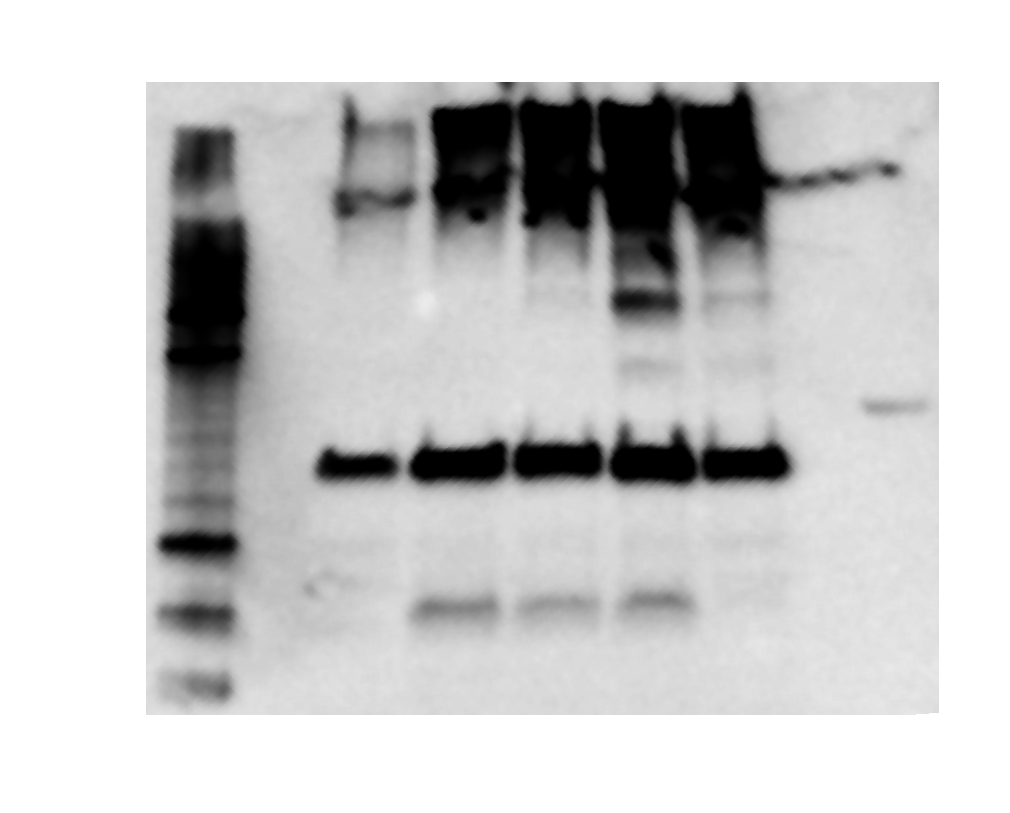
\includegraphics[width=\textwidth, trim={73 65 40 140}, clip, grid=true]{/Users/joehealey/Documents/Warwick/PhD/Thesis/chapters/chapter5/img/pET15b_expression_trial_pnf13.pdf}}
	\put(-165, 90){\rotatebox{45}{\textbf{His-Tag Marker}}}
	\put(-130, 90){\rotatebox{45}{\textbf{2 Hours}}}
	\put(-109, 90){\rotatebox{45}{\textbf{4 Hours}}}
	\put(-87, 90){\rotatebox{45}{\textbf{6 Hours}}}
	\put(-66, 90){\rotatebox{45}{\textbf{8 Hours}}}
	\put(-47, 90){\rotatebox{45}{\textbf{24 Hours}}}
	\put(-13, 90){\rotatebox{45}{\textbf{Marker}}}
	\put(-220, 63){\textbf{80} kDa\customarrow{-3pt}{155}}
	\put(-220, 51){\textbf{60} kDa\customarrow{0pt}{180}}
	\put(-220, 41){\textbf{50} kDa\customarrow{2pt}{190}}
	\put(-220, 30){\textbf{40} kDa\customarrow{3pt}{202}}
	\put(-220, 18){\textbf{30} kDa\customarrow{4pt}{205}}
	\put(-220, 5){\textbf{20} kDa\customarrow{3pt}{200}}

	\captionsetup{singlelinecheck=off, justification=centering, font=footnotesize, aboveskip=10pt}
	\caption{}
	\end{subfigure}
	\quad
	\begin{subfigure}[h]{0.4\textwidth}
	\frame{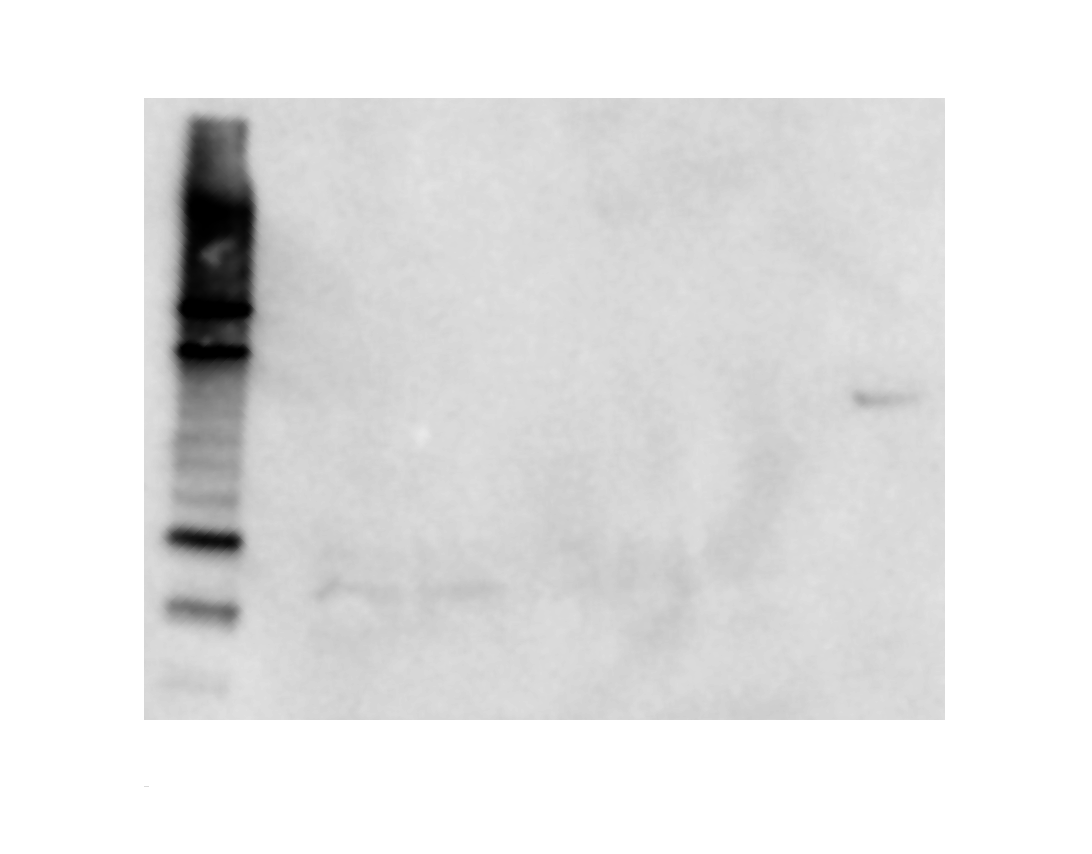
\includegraphics[width=\textwidth, trim={73 80 70 140}, clip, grid=true]{/Users/joehealey/Documents/Warwick/PhD/Thesis/chapters/chapter5/img/pET29a_expression_trial_pnf13.pdf}}
	\put(-165, 90){\rotatebox{45}{\textbf{His-Tag Marker}}}
	\put(-130, 90){\rotatebox{45}{\textbf{2 Hours}}}
	\put(-109, 90){\rotatebox{45}{\textbf{4 Hours}}}
	\put(-87, 90){\rotatebox{45}{\textbf{6 Hours}}}
	\put(-66, 90){\rotatebox{45}{\textbf{8 Hours}}}
	\put(-47, 90){\rotatebox{45}{\textbf{24 Hours}}}
	\put(-13, 90){\rotatebox{45}{\textbf{Marker}}}
	
	\captionsetup{singlelinecheck=off, justification=centering, font=footnotesize, aboveskip=10pt}
	\caption{}
	\end{subfigure}
	% Lane Labels
	%        X       

%	\put(-300,115){\textbf{pnf13 Monomer band \customarrow{6pt}{180}}}

	\captionsetup{singlelinecheck=off, justification=justified, font=footnotesize, aboveskip=10pt}
	\caption[pnf13 expression trial Western blot]{\textsc{\normalsize A Western blot of pnf13 expression in BL23(DE3) cells after induction.} \newline
	\textbf{(A)} Western blot of inductions of pnf13 from the pET15b vector, with an N-terminal Hexahistidine tag. \textbf{(B)} Western blot of inductions of pnf13 from the pET29a vector, with a C-terminal Hexahistidine tag. Good yields can be seen as early as 2 hours for the N-terminal tag -- No expression of C-terminally tagged pnf13 could be observed. Subsequent time points have been normalised to the same optical density, showing a roughly equivalent amount of protein on the gel, but higher yield in culture due to increased cell numbers.}
	\label{pnf13expressiontrial}
\end{figure}
\begin{figure}[p]
\thisfloatpagestyle{IHA-fancy-style}

	\centering
	\hspace{1cm}
	\begin{subfigure}[h]{0.4\textwidth}
		\frame{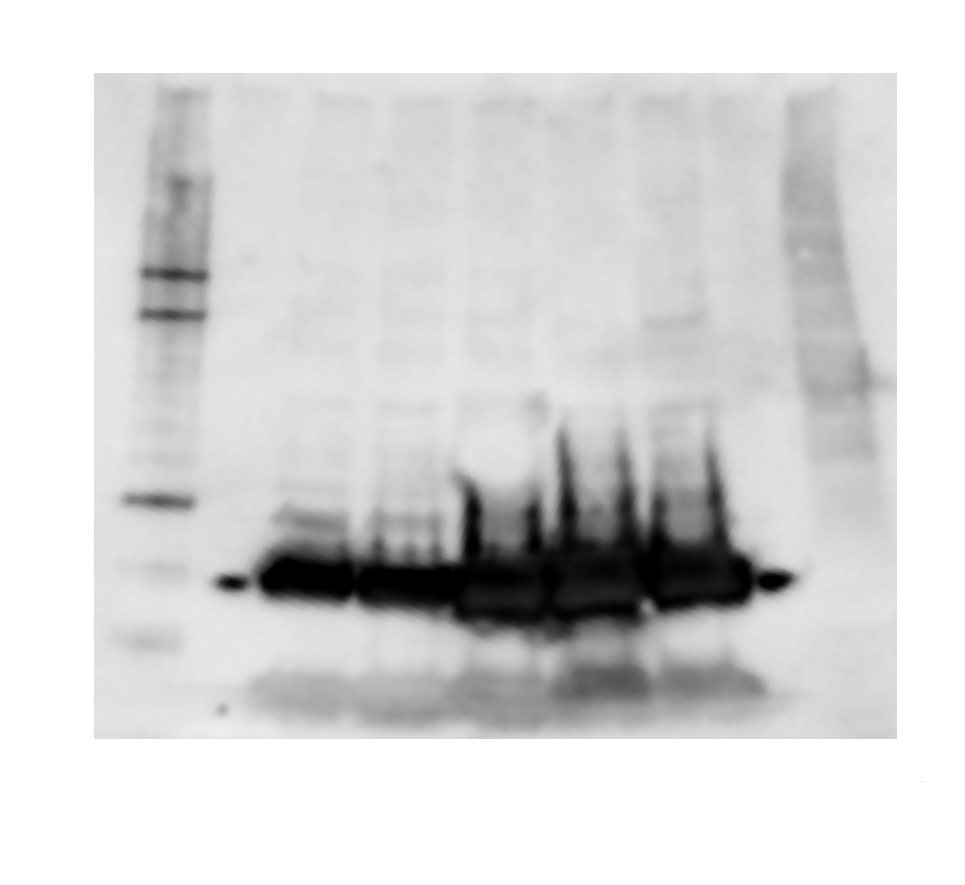
\includegraphics[width=\textwidth, trim={50 90 35 158 }, clip, grid=true]{/Users/joehealey/Documents/Warwick/PhD/Thesis/chapters/chapter5/img/pET15b_expression_trial_lumt13.pdf}}
	\put(-165, 86){\rotatebox{45}{\textbf{His-Tag Marker}}}
	\put(-130, 86){\rotatebox{45}{\textbf{2 Hours}}}
	\put(-109, 86){\rotatebox{45}{\textbf{4 Hours}}}
	\put(-87, 86){\rotatebox{45}{\textbf{6 Hours}}}
	\put(-66, 86){\rotatebox{45}{\textbf{8 Hours}}}
	\put(-47, 86){\rotatebox{45}{\textbf{24 Hours}}}
	\put(-13, 86){\rotatebox{45}{\textbf{Marker}}}
	\put(-220, 49){\textbf{40} kDa\customarrow{1pt}{180}}
	\put(-220, 39){\textbf{30} kDa\customarrow{1pt}{180}}
	\put(-220, 23){\textbf{20} kDa\customarrow{1pt}{180}}
	\put(-220, 8){\textbf{15} kDa\customarrow{1pt}{180}}

	\captionsetup{singlelinecheck=off, justification=centering, font=footnotesize, aboveskip=10pt}
	\caption{}
	\end{subfigure}
	\quad
	\begin{subfigure}[h]{0.4\textwidth}
	\frame{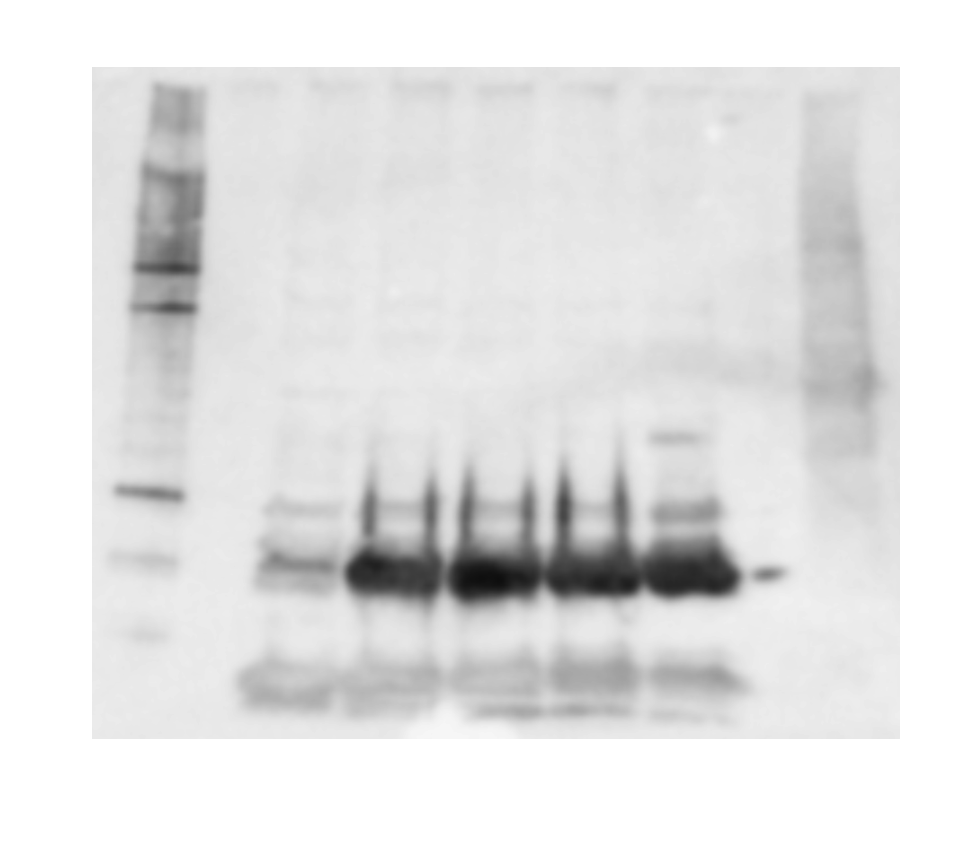
\includegraphics[width=\textwidth, trim={50 80 35 150 }, clip, grid=true]{/Users/joehealey/Documents/Warwick/PhD/Thesis/chapters/chapter5/img/pET29a_expression_trial_lumt13.pdf}}
	\put(-165, 86){\rotatebox{45}{\textbf{His-Tag Marker}}}
	\put(-130, 86){\rotatebox{45}{\textbf{2 Hours}}}
	\put(-109, 86){\rotatebox{45}{\textbf{4 Hours}}}
	\put(-87, 86){\rotatebox{45}{\textbf{6 Hours}}}
	\put(-66, 86){\rotatebox{45}{\textbf{8 Hours}}}
	\put(-47, 86){\rotatebox{45}{\textbf{24 Hours}}}
	\put(-13, 86){\rotatebox{45}{\textbf{Marker}}}
	
	\captionsetup{singlelinecheck=off, justification=centering, font=footnotesize, aboveskip=10pt}
	\caption{}
	\end{subfigure}
	% Lane Labels
	%        X       

%	\put(-300,115){\textbf{pnf13 Monomer band \customarrow{6pt}{180}}}

	\captionsetup{singlelinecheck=off, justification=justified, font=footnotesize, aboveskip=10pt}
	\caption[lumt13 expression trial Western blot]{\textsc{\normalsize A Western blot of lumt13 expression in BL23(DE3) cells after induction.} \newline
	\textbf{(A)} Western blot of inductions of lumt13 from the pET15b vector, with an N-terminal Hexahistidine tag. \textbf{(B)} Western blot of inductions of lumt13 from the pET29a vector, with a C-terminal Hexahistidine tag. Good yields can be seen as early as 2 hours for the N-terminal and C-terminal tags, with greater expression from the N-terminal (pET15b) clones. Subsequent time points have been normalised to the same optical density, showing a roughly equivalent amount of protein on the gel, but higher yield in culture due to increased cell numbers.}
	\label{lumt13expressiontrial}
\end{figure}
\hfill


\subsubsection{IMAC Purification and Polishing}
Purification was performed via Immobilised Metal ion Affinity Chromatography (``IMAC"), with Nickel$^{2+}$ as the metal ion, and sample polishing was done with a Superdex200 gel filtration column. Each sample was able to be purified well, particularly in the case of lumt13, where it was not uncommon to recover in excess of 100 mg of protein from two litres of bacterial culture. Purification was performed using an \"Akta FPLC system and a gradient elution (or gravity flow resin chromatography). Over the course of this project, multiple rounds of purification were performed, but the chromatogram trace was not highly reproducible, and had broad peaks; as a result, SDS-PAGEs were run on candidate fractions to identify the purest ones. Given the potential trimeric nature of the tail fibres, three hexahistidine tags would be present per final protein structure. A potential explanation for the unusual chromatograms could, therefore be, that stochastically, some proteins manage to bind one, two, or three histidine tags, resulting in differences in binding strength. It might be expected, in this case, that three peaks would result as the affinity of each multiple binding is reached and subsequently eluted, though this wasn't commonly observed, so something more complicated may be occurring. It is also possible that the tail fibres putative `extruded' shape may impede their flow into and out of the column, even when the dissociation point is reached, causing an extended elution peak. One final potential explanation could be that, given the putative nature of the tail fibres as binding structures, they themselves may be quite `sticky' and are therefore interacting with the column or other binding partners as yet unknown.

\begin{figure}[H]
	\vspace{0.2cm}
	\centering
	\begin{subfigure}[h]{0.45\textwidth}
		\frame{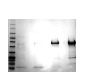
\includegraphics[width=\textwidth, trim={3.9 15 11.8 16 }, clip, grid=true]{/Users/joehealey/Documents/Warwick/PhD/Thesis/chapters/chapter5/img/pnf13_after_gel_filtration_concentrated.pdf}}
	\captionsetup{singlelinecheck=off, justification=centering, font=footnotesize, aboveskip=10pt}
	\caption{}
	\end{subfigure}
	\quad
	\begin{subfigure}[h]{0.45\textwidth}
	\frame{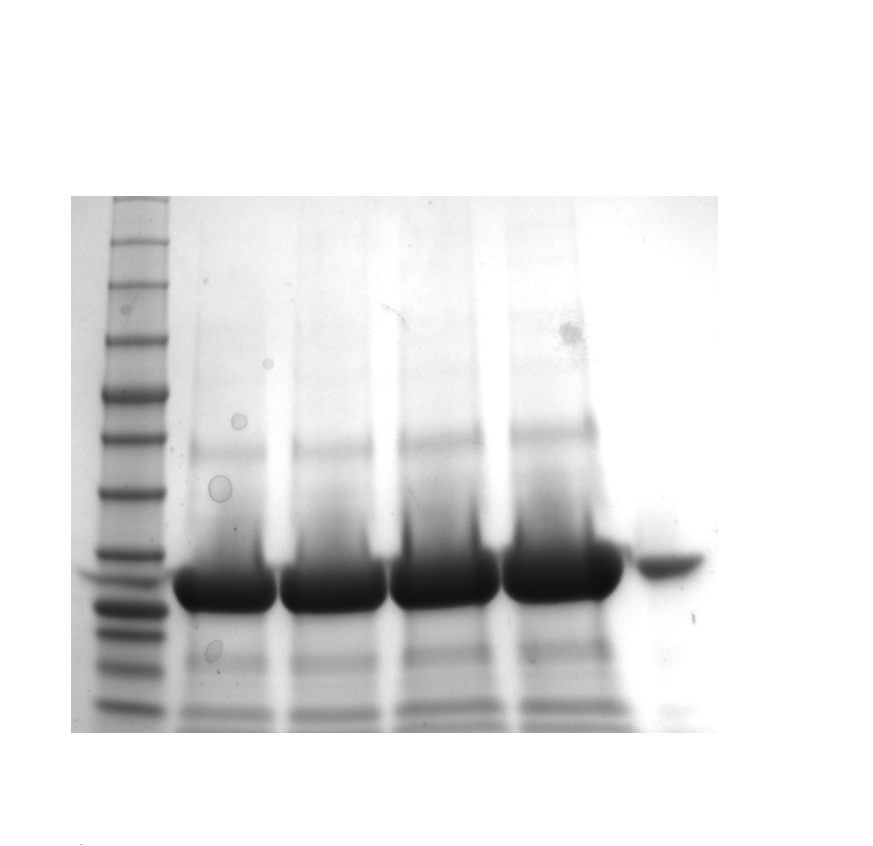
\includegraphics[width=\textwidth, trim={44 100 70 223 }, clip, grid=true]{/Users/joehealey/Documents/Warwick/PhD/Thesis/chapters/chapter5/img/lumt13_after_gel_filtration_concentrated.pdf}}
	\captionsetup{singlelinecheck=off, justification=centering, font=footnotesize, aboveskip=10pt}
	\caption{}
	\end{subfigure}
	% Lane Labels
	%        X       
%	\put(-300,115){\textbf{pnf13 Monomer band \customarrow{6pt}{180}}}

	\captionsetup{singlelinecheck=off, justification=justified, font=footnotesize, aboveskip=10pt}
	\caption[Tail fibre chromatographic preparations]{\textsc{\normalsize SDS-PAGE gels of the PVC tail fibres purified from pET15b.} \vspace{0.1cm} \newline
	\textbf{(A)} Stained SDS-PAGE gel of pnf13 expressed from pET15b, from several fractions across the elution profile from IMAC, after concentration with Amicon centrifugal columns. Sample is approaching purity. \textbf{(B)} Staining of SDS-PAGE gel of lumt13 expressed from pET15b, from several fractions from across the elution profile, after concentration with Amicon centrifugal columns. Samples are approaching purity. The difference in expression levels between pnf13 and lumt13 is apparent. Final polishing was conducted via gel filtration with a Superdex 200 Increase column.}
	\label{gelpurifications}
\end{figure}

\subsection{Structural Analyses}

\subsubsection{Trimerism of PVC Tail Fibre Proteins}
During routine SDS-PAGE while running expression and purification experiments, it was observed that the tail fibres often did not readily migrate in to the acrylamide (this can be seen in \vref{trimerism}). A standard SDS-PAGE set up included boiling the sample in the presence of gel loading dye, containing DTT, $\beta$-mercaptoethanol and SDS, which ordinarily would be more than enough chemical and physical disruption to denature most proteins. Better, though in the case of pnf13, not complete, denaturation could be coerced with the presence of urea at roughly 8 M, and the inclusion of EDTA in the loading dye. This thermal/chemical stability is a known hallmark of $\beta$-stranded fibre proteins and is a valuable indication of the true structure and correct fold of these proteins \citep{Papanikolopoulou2008, Gazit2008}

\begin{figure}[h]
 \thisfloatpagestyle{IHA-fancy-style}
	\centering
	\frame{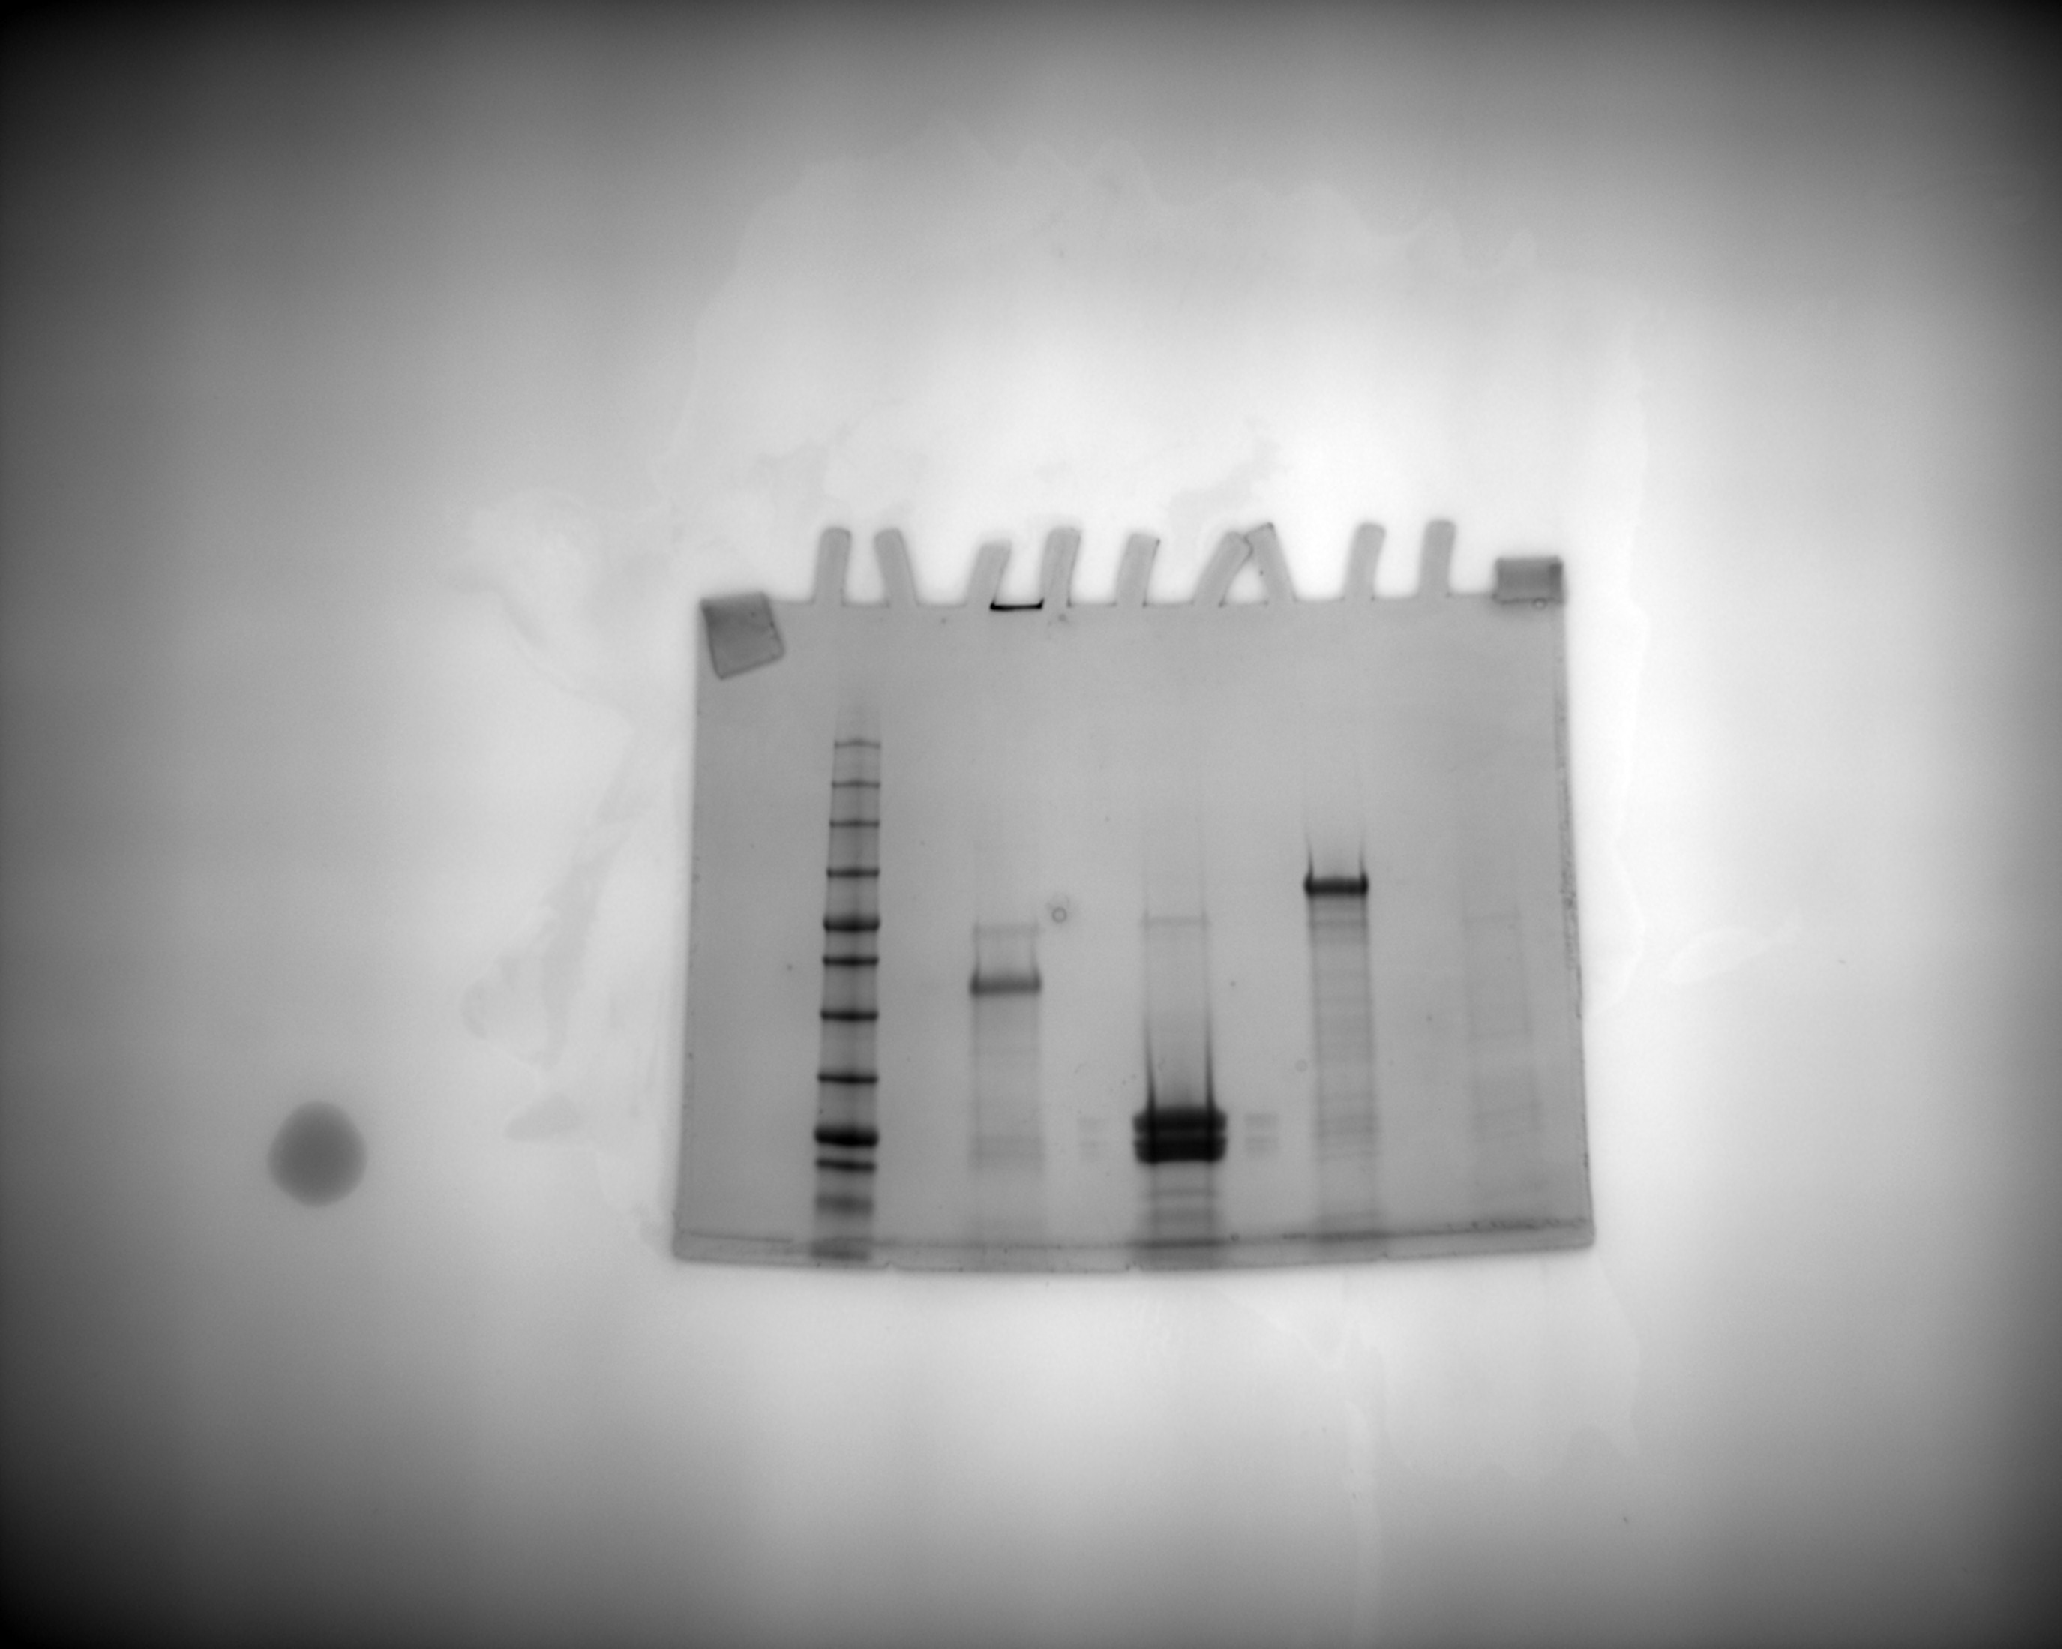
\includegraphics[width=0.4\textwidth, trim={375 180 390 280}, clip]{/Users/joehealey/Documents/Warwick/PhD/Thesis/chapters/chapter5/img/multimerism.pdf}}
	% Lane Labels
	%        X       Y
	\put(-34,255){\rotatebox{45}{lumt13}}
	\put(-150,260){\rotatebox{45}{Marker}}
	\put(-94,260){\rotatebox{45}{pnf13}}
	\put(-201,240){\textbf{kDa}}
	% Ladder Labels
                                                             %{Height}{Rotation}
	\put(-205,189){\textbf{245}\customarrow{1pt}{180} }
	\put(-205,175){\textbf{190}\customarrow{1pt}{180} }
	\put(-205,160){\textbf{135}\customarrow{1pt}{180} }
	\put(-205,143){\textbf{100}\customarrow{1pt}{180} }
	\put(-205,124){\textbf{\ \ 80}\customarrow{1pt}{180} }
	\put(-205,110){\textbf{\ \ 58}\customarrow{1pt}{180} }
	\put(-205,90){\textbf{\ \ 46}\customarrow{1pt}{180} }
	\put(-205,72){\textbf{\ \ 32}\customarrow{1pt}{180} }
	\put(-205,51){\textbf{\ \ 25}\customarrow{1pt}{180} }
	\put(-205,35){\textbf{\ \ 22}\customarrow{1pt}{180} }
	\put(-205,22){\textbf{\ \ 17}\customarrow{1pt}{180} }
	\put(-205,5){\textbf{\ \ 11}\customarrow{1pt}{180}}
	% Annotations
	\put(-80,90){\textbf{\customarrow{3pt}{320} pnf13 Monomer}}
	\put(-80,138){\textbf{\customarrow{-6pt}{30} pnf13 Dimer}}
	\put(-80,230){\textbf{\customarrow{2pt}{320} pnf13 Trimer}}
	\put(-10,50){\textbf{\customarrow{1pt}{0} lumt13 Monomer}}
	\put(-10,122){\textbf{\customarrow{1pt}{330} lumt13 Trimer}}

	\captionsetup{singlelinecheck=off, justification=justified, font=footnotesize, aboveskip=10pt}
	\caption[Trimeric nature of PVC tail fibres]{\textsc{\normalsize Trimerism of PVC tail fibres revealed via SDS-PAGE}\vspace{0.1cm}\newline An example of a routine SDS-PAGE gel for semi-purified (post IMAC) tail fibre proteins (pnf13 and lumt13). Despite being a denaturing gel, where the the input samples were boiled in SDS loading dye with urea, multimeric forms of the proteins can be seen, demonstrating the stability of the tail fibres. Trimeric, dimeric and monomeric forms of pnf13 are identifiable (the trimeric form remains in the well at the top of the gel). For lumt13, monomeric and trimeric forms are apparent. Dimeric forms are seemingly sufficiently unstable that they entirely denature completely to monomers, if the trimers denature at all.}
	
	\label{trimerism}
\end{figure}
\clearpage

\subsubsection{Thermal Stability and Secondary Structure Studies via Circular Dichroism}
Upon observing the stability of the tail fibres in denaturing conditions, it was decided to examine this thermal stability further via temperature ramping circular dichroism experiments, from which it is also possible to get secondary structure and to get an indication of whether the folding of the proteins is occurring correctly. Figures \ref{pnfmelt} and \ref{lumtmelt} show a composite of 15 spectra each, acquired at 5\degC{} increments and coloured by temperature. Each spectrum was acquired six times (technical replicates) in each run, and for each protein, three runs were performed at separate times, each with a different protein preparation to ensure consistency of purifications (biological replicates). For pnf13, spectra were run at 0.1\mgml and for lumt13, at 0.25\mgml. Concentrations for each run were determined empirically prior to setting up the temperature ramp, by sequentially two-fold diluting a 1\mgml stock of each protein until the CD spectrometer HT voltage did not exceed $\approx$600 V at 190 nm. While spectra were collected from 260 to 185 nm, without extremely pure buffers and high quality light sources (typically synchrotrons), CD data becomes very noisy at lower wavelengths as many molecules begin to absorb around the 190 nm region. Consequently, only data down to 190 nm was included for analysis. All spectra are baseline subtracted against the buffer control (Sodium fluoride).

A transition can be seen as the two extremes of temperature are separated on the graph. Characteristically, this occurred at approximately 65\degC, for pnf13 - putatively signalling the start of unfolding. At higher temperatures, the $\beta$-sheet signal actually intensified. For lumt13, the major collapse of secondary structure appears between 50 and 60\degC, but no other structure seems to appear at higher temperatures. In both cases, even up to 95\degC, secondary structure seemingly persists as the signal is not abolished completely, though the structure is almost certainly no longer in its native form.


\begin{figure}[p]
\thisfloatpagestyle{IHA-fancy-style}

	\centering
	\includegraphics[width=0.85\textwidth,  trim={0, 0, 10, 0}, clip]{/Users/joehealey/Documents/Warwick/PhD/Thesis/chapters/chapter5/img/pnf_AvgRun_CD_melt_2D.pdf}
	\captionsetup{singlelinecheck=off, justification=justified, font=footnotesize, aboveskip=10pt}
	\caption[pnf13 CD melt plot]{\textsc{\normalsize CD temperature ramping spectra for pnf13}\vspace{0.1cm} \newline A composite of 15 CD melt spectra from the temperature ramping experiment for pnf13 (from 20\degC{} to 95\degC{} in 5\degC{} increments). These are average spectra from 3 biological replicates (each of which in turn is an average of 6 technical replicate spectra accumulations). Cooler colours (purple) correspond to lower temperature spectra, and warmer colours (yellow-orange) correspond to higher temperature spectra.}
	\label{pnfmelt}
	\end{figure}
	
\begin{figure}[p]
\thisfloatpagestyle{IHA-fancy-style}

	\centering
	\includegraphics[width=0.85\textwidth, trim={0, 0, 10, 0}, clip]{/Users/joehealey/Documents/Warwick/PhD/Thesis/chapters/chapter5/img/lumt_CD_melt_2D.pdf}
	\captionsetup{singlelinecheck=off, justification=justified, font=footnotesize, aboveskip=10pt}
	\caption[lumt13 CD melt plot]{\textsc{\normalsize CD temperature ramping spectra for lumt13}\vspace{0.1cm} \newline A composite of 15 CD melt spectra from the temperature ramping experiment for lumt13 (from 20\degC{} to 95\degC{} in 5\degC{} increments). These are average spectra from 3 biological replicates (each of which in turn is an average of 6 technical replicate spectra accumulations). Cooler colours (purple) correspond to lower temperature spectra, and warmer colours (yellow-orange) correspond to higher temperature spectra.}
	\label{lumtmelt}
\end{figure}

\subsubsection{Secondary Structure Prediction via Dichroweb}
As mentioned, one of the primary reasons to conduct circular dichroism studies is to gather information about the secondary structure of a protein. Through use of tools like Dichroweb, input spectra can be deconvoluted and compared to the CD spectra for other proteins of known structure. By doing so, the secondary structure for the unknown candidate protein can be approximated \citep{Whitmore2004, Lobley2002}. Each of the 45 spectra for each protein (15 spectra per biological replicate) were analysed, and the resulting secondary structure proportions average for each temperature between the three runs, thus reporting the average secondary structure across the replicates and temperature curve.

\myparagraph{Algorithm and reference set selection}
For calculation, the CDSSTR algorithm \citep{Compton1986,Sreerama2000b, Manavalan1987} was chosen for a number of reasons. Firstly, it is cited as being one of, if not the most accurate algorithms for circular dichroism (having superseded a number of the others), but with the tradeoff of increased run-time, though that was not a concern for this analysis. Secondly, it is compatible with the spectra reference set chosen (see the following section), and the wavelengths captured (some algorithms require sub-190 nm data, which was available, but considerably more noisy as seen in \vrefrange{pnfmelt}{lumtmelt}). The other options for the dataset range available: SELCON, CONTIN and K2D all fail to match the accuracy of CDSSTR in testing here. K2D doesn't require a reference set but provided the worst Normalised Root-Mean-Square-Deviation (NRMSD) values by a significant margin (see \vref{K2D}), and only analyses spectra to 200 nm.

Fitting quality was trialled with a number of reference sets compatible with the scan parameters and algorithms available (this immediately limited choices to only a couple of reference sets). It was decided to proceed with reference set 7, as it contains the largest number of non-specialist proteins (i.e. non-membraneous etc.), and also because it contained spectral information for denatured proteins, which for the denaturing gradients seemed likely to give the best representation of the spectra \citep{Sreerama2000b,Sreerama2000a}. Full details of all the spectra can be found at the Dichroweb site\footnote{\url{http://dichroweb.cryst.bbk.ac.uk/html/userguide_datasets.shtml}}. Reference set 4 also gave good results in testing, but as Set 7 contains all of Set 4's proteins in addition to extras, including denatured forms as mentioned, it was adopted instead. Set 6 was also able to give decent spectra fits, but uses the full 185 nm data range; without extremely high quality experimental materials and access to a synchrotron, it is typically considered unwise to analyse beyond 190 nm.

As an example of the improved results obtained from use of the CDSSTR and the chosen reference set, spectra are shown in \vref{dichrowebalgos} for one of the input spectra tested under several models. Dichroweb further provides an NRMSD statistic \citep{Mao1982}, to quantitatively assess the least squares goodness of fit.

\begin{figure}[p]
\thisfloatpagestyle{IHA-fancy-style}

	%\vspace{0.2cm}
	\centering
	\begin{subfigure}[h]{0.49\textwidth}
	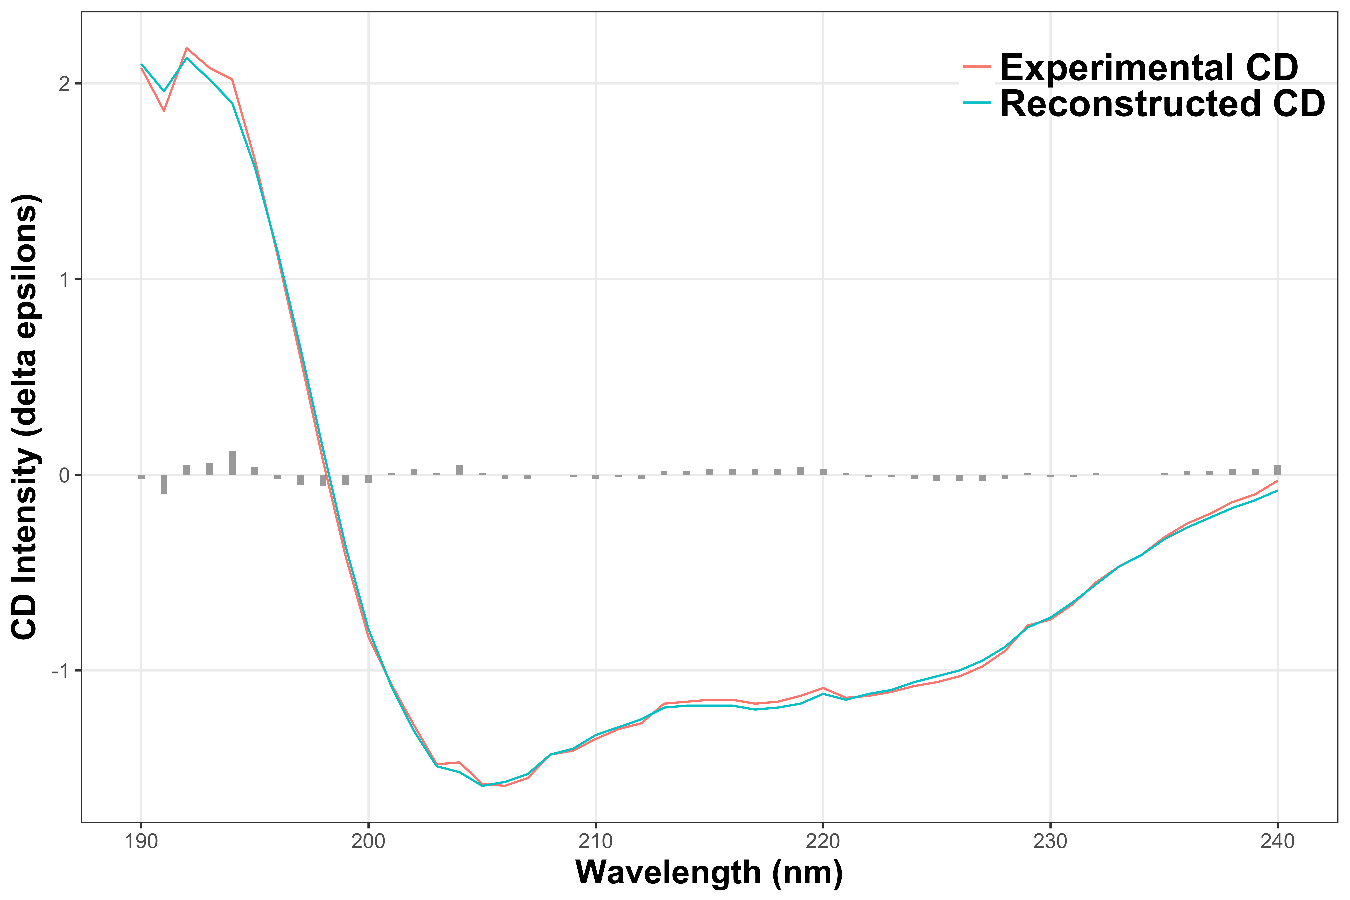
\includegraphics[width=\textwidth, trim={0 0 0 0}, clip, grid=true]{/Users/joehealey/Documents/Warwick/PhD/Thesis/chapters/chapter5/img/lumt13_R1S1_CDSSTRSet7.pdf}
	\put(-47,15){\textsf{\textbf{\tiny NRMSD $= 0.03$}}}
	\captionsetup{singlelinecheck=off, justification=centering, font=footnotesize, aboveskip=10pt}
	\caption{}
	\end{subfigure}
	\begin{subfigure}[h]{0.49\textwidth}
	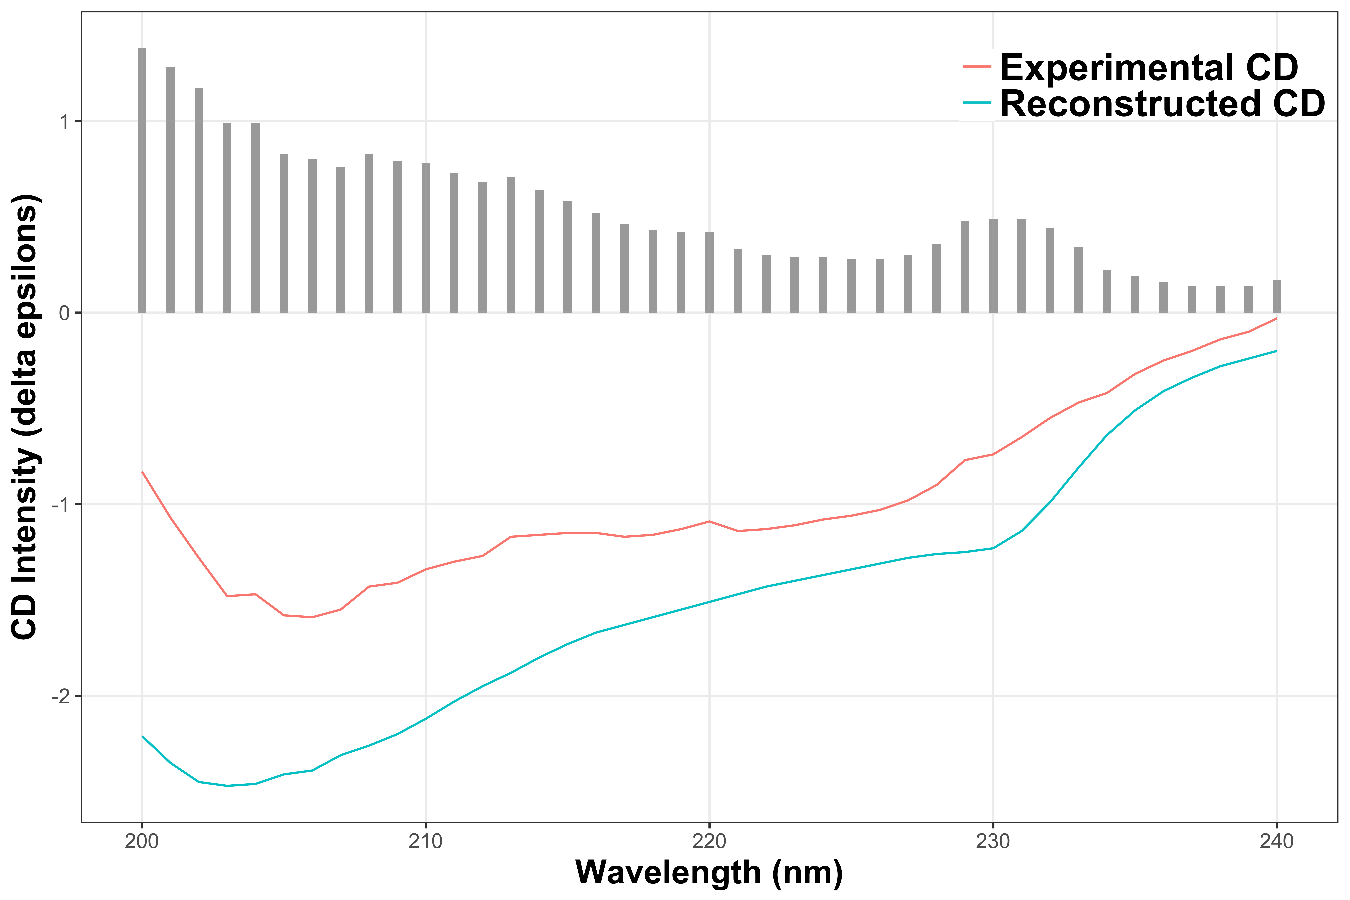
\includegraphics[width=\textwidth, trim={0 0 0 0}, clip, grid=true]{/Users/joehealey/Documents/Warwick/PhD/Thesis/chapters/chapter5/img/lumt13_R1S1_K2D.pdf}
	\put(-47,15){\textsf{\textbf{\tiny NRMSD $= 0.585$}}}
	\captionsetup{singlelinecheck=off, justification=centering, font=footnotesize, aboveskip=10pt}
	\caption{}
	\label{K2D}
	\end{subfigure}

	\begin{subfigure}[h]{0.49\textwidth}
	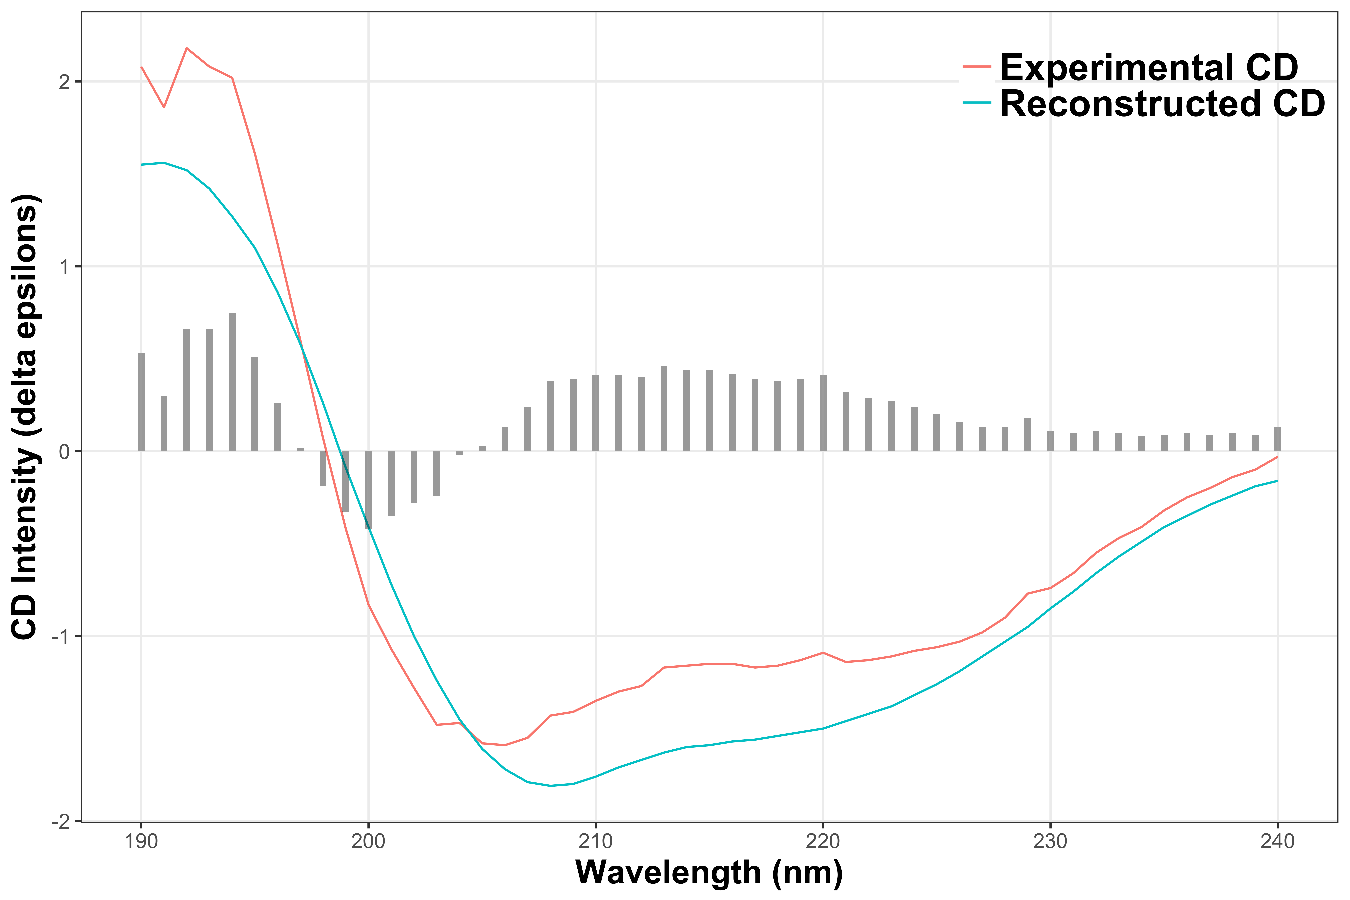
\includegraphics[width=\textwidth, trim={0 0 0 0}, clip, grid=true]{/Users/joehealey/Documents/Warwick/PhD/Thesis/chapters/chapter5/img/lumt13_R1S1_Selcon4.pdf}
	  \put(-47,15){\textsf{\textbf{\tiny NRMSD $= 0.273$}}}
	\captionsetup{singlelinecheck=off, justification=centering, font=footnotesize, aboveskip=10pt}
	\caption{}
	\end{subfigure}
	\begin{subfigure}[h]{0.49\textwidth}
	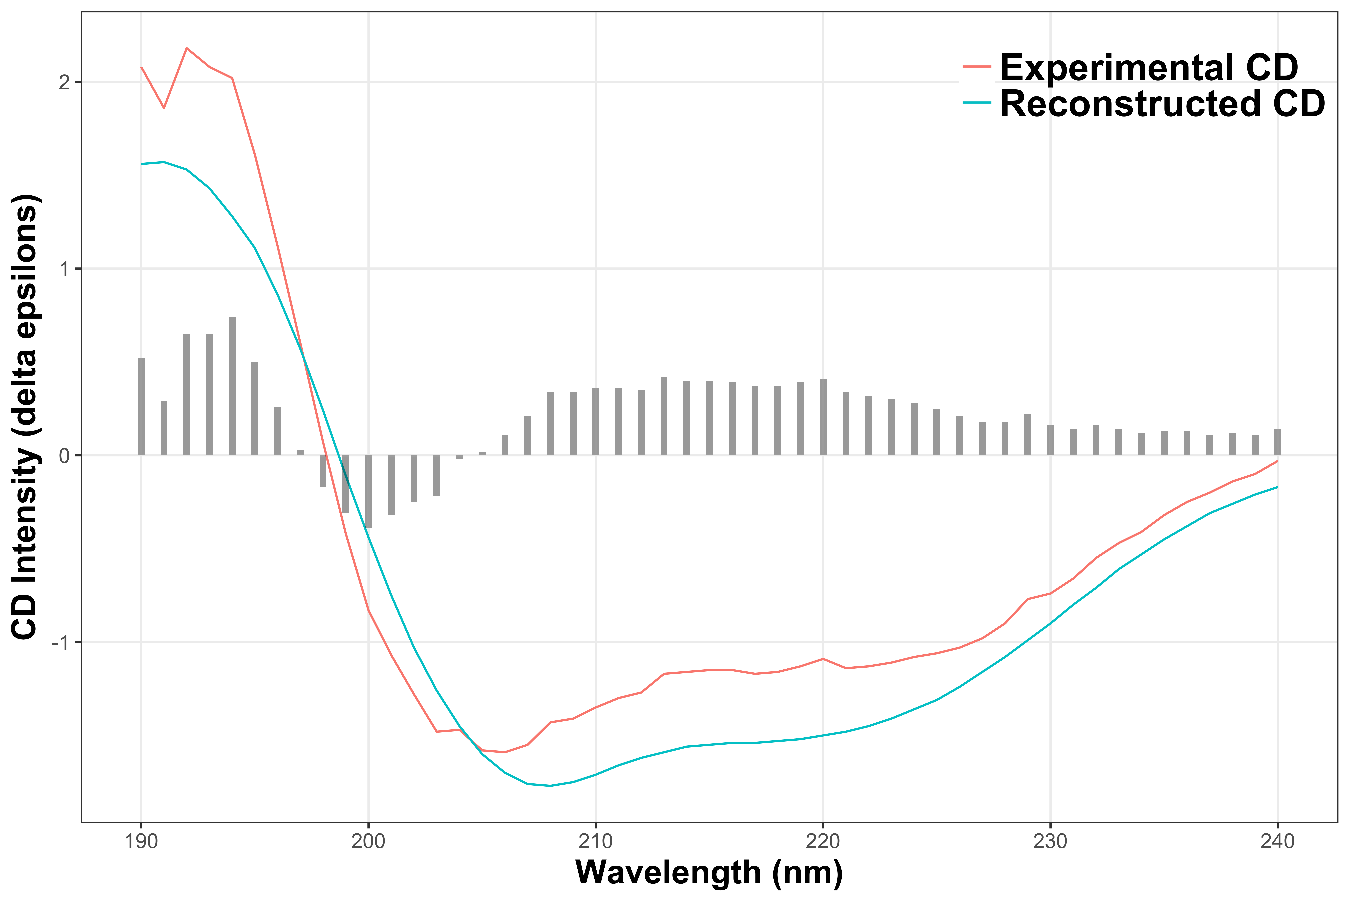
\includegraphics[width=\textwidth, trim={0 0 0 0}, clip, grid=true]{/Users/joehealey/Documents/Warwick/PhD/Thesis/chapters/chapter5/img/lumt13_R1S1_Selcon7.pdf}
	  \put(-47,15){\textsf{\textbf{\tiny NRMSD $= 0.271$}}}
	\captionsetup{singlelinecheck=off, justification=centering, font=footnotesize, aboveskip=10pt}
	\caption{}
	\end{subfigure}
	
	\begin{subfigure}[h]{0.49\textwidth}
	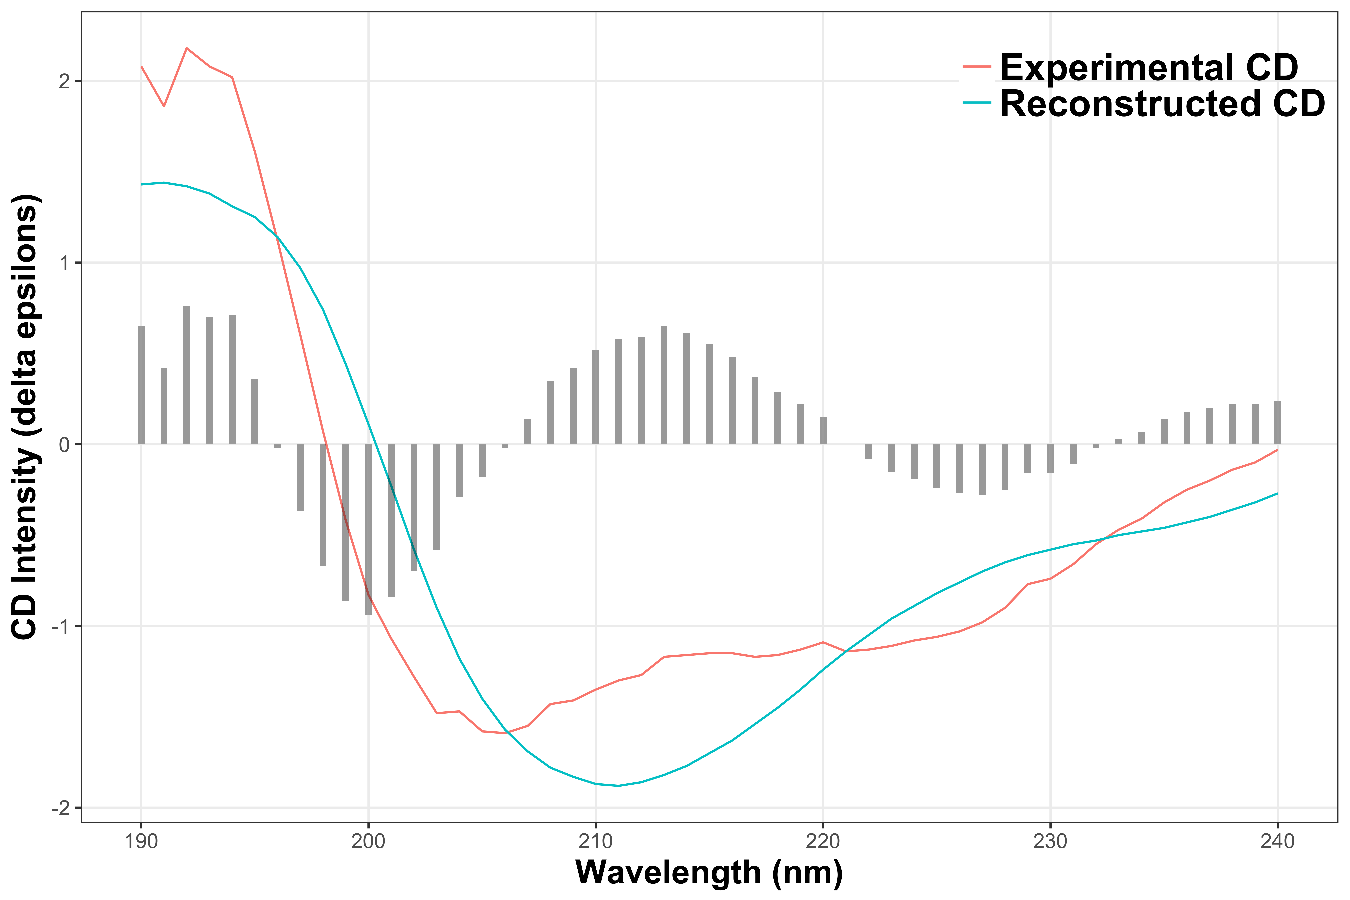
\includegraphics[width=\textwidth, trim={0 0 0 0}, clip, grid=true]{/Users/joehealey/Documents/Warwick/PhD/Thesis/chapters/chapter5/img/lumt13_R1S1_Contin4.pdf}
	  \put(-47,15){\textsf{\textbf{\tiny NRMSD $= 0.368$}}}
	\captionsetup{singlelinecheck=off, justification=centering, font=footnotesize, aboveskip=10pt}
	\caption{}
	\end{subfigure}
	\begin{subfigure}[h]{0.49\textwidth}
	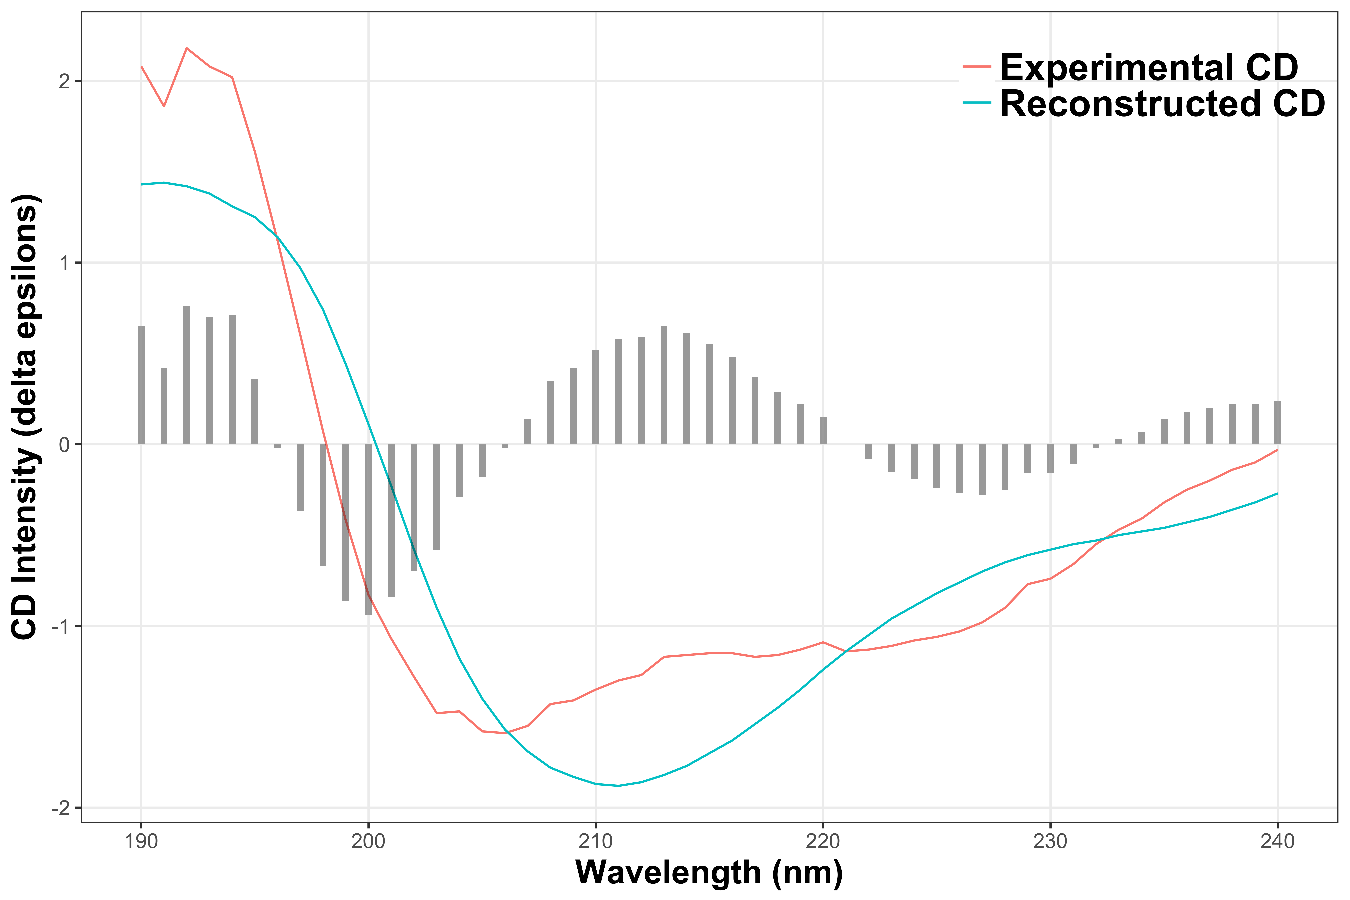
\includegraphics[width=\textwidth, trim={0 0 0 0}, clip, grid=true]{/Users/joehealey/Documents/Warwick/PhD/Thesis/chapters/chapter5/img/lumt13_R1S1_Contin7.pdf}
	  \put(-47,15){\textsf{\textbf{\tiny NRMSD $= 0.368$}}}
	\captionsetup{singlelinecheck=off, justification=centering, font=footnotesize, aboveskip=10pt}
	\caption{}
	\end{subfigure}
	
	\captionsetup{singlelinecheck=off, justification=justified, font=footnotesize, aboveskip=10pt}
	\caption[Comparisons of Dichroweb algorithms and reference sets]{\textsc{\normalsize Comparisons of optimal Dichroweb algorithms and reference sets.} \vspace{0.1cm} \newline Each of these charts shows a comparison of a different algorithm and reference set for identifying the optimal parameters for estimation of secondary structure proportions from the acquired spectra. As an example, each spectra shows the result for the 20\degC{} spectra for lumt13 when analysed with a selection of compatible reference sets and algorithms. Pink lines are the experimental spectral data, and cyan lines are the reconstructed reference data. light grey bars depict the residual difference between the 2 line spectra at that point to highlight the disparity. \textbf{(A)} The optimal solution from this testing, of the lumt13 spectra analysed using CDSSTR and reference set 7. \textbf{(B)} Analysis result from the K2D algorithm, which does not require a reference set. \textbf{(C)} Result of spectral analysis using the SELCON algorithm and reference set 4. \textbf{(D)} Result of spectral analysis using the SELCON algorithm and reference set 7. \textbf{(E)} Result of spectral analysis using the CONTIN algorithm and reference set 4. \textbf{(F)} Result of spectral analysis using the CONTIN algorithm and reference set 7. Note there is little to no difference in the use of set 4 or set 7.}
	\label{dichrowebalgos}
\end{figure}



\myparagraph{Secondary structure predictions}
With optimal parameters for secondary structure calculation through Dichroweb identified, all spectra were analysed for their relative secondary structure proportions. \vref{tailfibresbars} shows the relative proportions according to Dichroweb, plotted as stacked bars. The increasing temperatures are plotted along the y-axis, and the percentage of each secondary structure type long the x-axis. Dichroweb recognises 6 classes of secondary structure, including 2 types of both $\alpha$-helix and $\beta$-sheet. Respectively these are: ``Helix1" - regular $\alpha$-helix, ``Helix2" - `distorted' $\alpha$-helix, likewise for ``Strand" 1 and 2, and finally unstructured turn and unordered regions. 

\begin{figure}[p]
\thisfloatpagestyle{IHA-fancy-style}

	\vspace{-0.2cm}
	\centering
	\begin{subfigure}{\textwidth}
	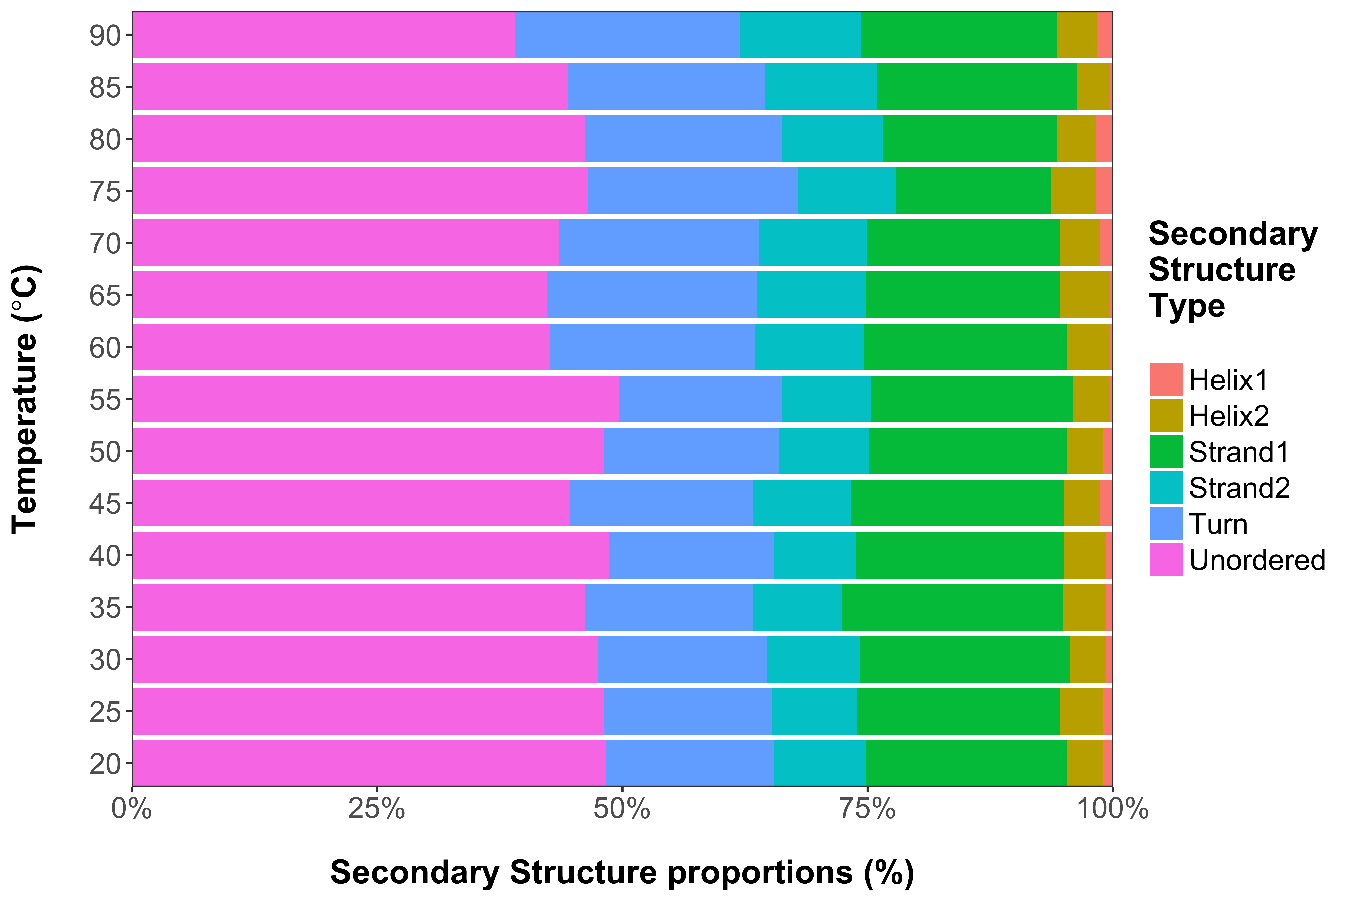
\includegraphics[width=\textwidth, trim={0 0 0 0}, clip, grid=true]{/Users/joehealey/Documents/Warwick/PhD/Thesis/chapters/chapter5/img/Pnf_avg_SS.pdf}
	\captionsetup{singlelinecheck=off, justification=centering, font=footnotesize, aboveskip=7pt}
	\caption{}
	\label{pnfss}
	\end{subfigure}
	
	\begin{subfigure}{\textwidth}
	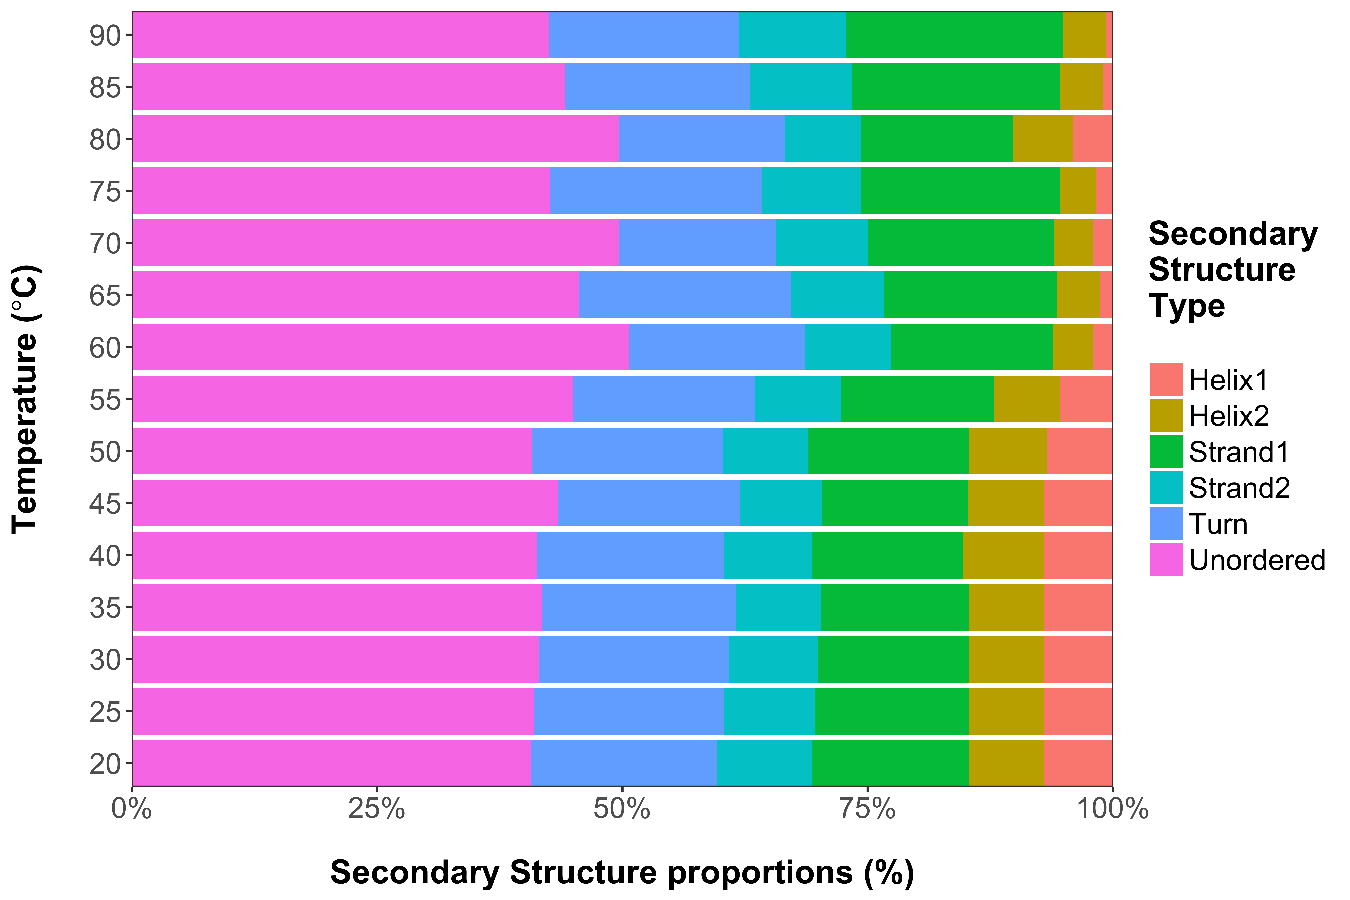
\includegraphics[width=\textwidth, trim={0 0 0 0}, clip, grid=true]{/Users/joehealey/Documents/Warwick/PhD/Thesis/chapters/chapter5/img/Lumt_avg_SS.pdf}
	\captionsetup{singlelinecheck=off, justification=centering, font=footnotesize, aboveskip=7pt}
	\caption{}
	\label{lumtss}
	\end{subfigure}
	
	\captionsetup{singlelinecheck=off, justification=justified, font=footnotesize, aboveskip=8pt}
	\caption[PVC Tail fibre secondary structure proportions across the melting gradient]{\textsc{\normalsize CD melt secondary structure proportions for tail fibre proteins.} \vspace{0.1cm} \newline Stacked bar charts showing the proportions of secondary structure as estimated by Dichroweb, for averages of the 3 replicate spectra, for each protein at 15 different temperatures in the melting gradient experiment.\textbf{(A)} Secondary structure proportions for pnf13. \textbf{(B)} Secondary structure proportions for lumt13. ``Helix1" - regular $\alpha$-helix, ``Helix2" - `distorted' $\alpha$-helix, ``Strand 1" - regular $\beta$-sheet, ``Strand 2" - distorted $\beta$-sheet, ``Turn" - turns/loops, ``Unordered" - No canonical secondary structure.}
	\label{tailfibresbars}
\end{figure}

\newpage
\subsubsection{Comparisons with Known Structures}\label{comparisons}
The cloned tail fibres from the PVCs appear to be dominated by unordered, turn, and $\beta$-sheet motifs. The assumption is made at this point that the tail fibres are likely to be folding correctly in to their native structures for the following reasons. Firstly, the `knitted' and interwoven trimeric nature of known tail fibres is unlike that of trimers of typical globular proteins, where they simply form three identical monomers which each have a functioning `lone' structure, and complex together. For tail fibres, the functional structure \emph{is} the trimeric form, and all three monomers have to contribute to form the structure. Each monomer on its own would not be capable of maintaining the extruded structure which will have energetically unfavourable regions exposed. The trimerism of known tail fibre structures is apparent from \vref{tailfibrestructures}, and for these tail fibres is reinforced by \vref{trimerism}. Secondly, the stability that was seen in the CD melt studies is characteristic of phage proteins, and tail fibre like proteins in particular. Thirdly, the ability to probe and purify via the histidine tag suggests that the proteins are not simply malformed and creating inclusion bodies etc., if that were the case, it would be expected that the histidine tags would be buried within the inclusions and purification would likely have failed.

However, to compare this directly to the published structures for validity, the secondary structure proportions for several existing tail fibre proteins was examined in two ways. Firstly, the `raw' secondary structure proportions were calculated directly from the PDB crystal structures via a bespoke script, using PyChimera \citep{Rodriguez-GuerraPedregal2018} and UCSF Chimera \citep{Pettersen2004}, which in turn assigns secondary structure using the well-known DSSP algorithm \citep{Kabsch1983}. Secondly, another web service from the groups behind Dichroweb, ``PDB2CD"\footnote{\url{http://pdb2cd.cryst.bbk.ac.uk/}}, simulates circular dichroism spectra from resolved structures, and thus the secondary structure of analogous proteins is compared here.

By way of example, the secondary structure proportions for the structures shown in \vref{tailfibrestructures}, and domain homologies detected by HHPred are reproduced in \vref{referenceSS}. Note, these results are extracted from DSSP assignments as mentioned in the last paragraph, however DSSP only recognises three classes of secondary structure (thus the percent helix according to DSSP represents the approximately the combined Helix 1 and Helix 2 that Dichroweb reports for the same structure, and so on).


\vref{pdb2cd} shows the same secondary structure calculations performed on the same set of structures, but instead, uses the data output by Dichroweb. While this abstracts the data from the crystal structure slightly, it makes the spectra more directly comparable to the data for the PVC tail fibre proteins. In order to obtain this data, circular dichroism spectra are simulated from the PDB depositions, using the webserver PDB2CD \citep{Mavridis2017}, and in turn passed back through Dichroweb. In this case, the CDSSTR algorithm was used, however PDB2CD uses the SP175 reference set \citep{Lees2006}, so this was also used with Dichroweb.

\footnotesize
\rowcolors{1}{gray!20}{white}
\begin{tabularx}{\textwidth}{Z C C C}
\hiderowcolors
\captionsetup{singlelinecheck=off, justification=justified, font=footnotesize, belowskip=5pt}
\caption[Secondary structure proportions of resolved tail fibres according to DSSP]{\textsc{\normalsize DSSP secondary structure proportions for resolved tail fibre proteins.} \vspace{0.1cm} \newline The secondary structure proportions for various tail fibre like proteins with resolved atomic structures in the PDB database, as determined by calculation directly from the atomic structure. The corresponding structures can be found in \vref{tailfibrestructures} and in \vref{domainstructure}, with the exception of PDB ID 1PDI, which, for an unknown reason, fails to have secondary structure assigned by DSSP/UCSF Chimera.}
\label{referenceSS}\\

PDB ID & \% Helix & \% Sheet & \% Other \\
\hline\hline
\showrowcolors
2XGF  & 2 & 16 & 82 \\
5NXF  & 5 & 9 & 86 \\
1QIU  & 7 & 26 & 67 \\
1H6W  & 7 & 6 & 87 \\
1V1H  & 4 & 18 & 78 \\
3IZO  & 13 & 18 & 70 \\
1OCY  & 5 & 2 & 93 \\
\hline
\end{tabularx}
\vspace{-0.6cm}
\rowcolors{1}{gray!20}{white}
\begin{tabularx}{\textwidth}{Z C C C C C C C}
\hiderowcolors
\captionsetup{singlelinecheck=off, justification=justified, font=footnotesize, belowskip=5pt}
\caption[Secondary structure proportions of resolved tail fibres]{\textsc{\normalsize Dichroweb secondary structure proportions for resolved tail fibre proteins.} \vspace{-0.3cm} \newline The secondary structures proportions for various tail fibres with resolved atomic structures in the PDB database, calculated via the PDB2CD and Dichroweb webservices.}
\label{pdb2cd}\\[-0.5em]
PDB ID & \% Helix 1 & \% Helix 2 & \% Sheet1 & \% Sheet 2 & \% Turn & \% Other & NRMSD \\
\hline\hline
\showrowcolors
2XGF & 2 & 8 & 23 & 13 & 12 & 42 & 0.027 \\
5NXF & 0 & 6 & 28 & 14 & 11 & 40 & 0.065 \\
1QIU & 0 & 6 & 26 & 14 & 11 & 42 & 0.048 \\
1H6W & 8 & 11 & 16 & 11 & 14 & 39 & 0.032 \\
1V1H & 0 & 6 & 26 & 14 & 11 & 42 & 0.035 \\
1OCY & 11 & 12 & 13 & 10 & 14 & 40 & 0.03 \\
3IZO & 5 & 10 & 17 & 11 & 14 & 42 & 0.033 \\
\hline

\end{tabularx}
\normalsize

Exploring the secondary structure of the resolved structures reveals that they are also dominated by $\beta$-sheet and `Other' secondary structure forms, though the agreement between direct calculation and simulated circular dichroism proportions is quite variable. Overall, $\alpha$-helical structural spans appear very limited in known tail fibres, and this trend is also seen in the tail fibres cloned from the PVCs, contributing to only around 10-15\% of the overall structure. Moreover, despite differing substantially in length, sequence and also having somewhat different melting profiles, the secondary structures of the PVCpnf13 and PVClumt13 fibres are roughly equivalent. This is therefore indicative of a robust `tail fibre' blueprint, in which the macrostructure is important, but the sequence specifics appear free to drift - potentially significantly. For instance, it appears the coordination of one or more metal ions is common (though maybe not obligatory), and yet, the sequences don't appear to preserve a distinct binding pattern, possibly suggesting that many different ions held by many different amino acids are all `valid solutions' to the problem of creating a tail fibre type protein.


\subsubsection{Crystallography}
Since the tail fibres were able to be expressed to reasonable quantities, some crystallographic screens were attempted, as it's the approach with greatest previous success, as mentioned in \vref{tailfibreintro}.

With lumt13, crystals were obtained in 12 conditions, in under a week. Since it is not uncommon for crystallisation screens to result in no crystals at all, even after months or years of incubation, it seemed that crystallisation was a promising approach for these proteins. \vref{crystalconditionstable} shows the buffer conditions for which crystals could be seen. \vref{crystals} shows a selection of the morphologies obtained. Unfortunately, the reduced yield and purity of the pnf13 tail fibre meant that it was not possible to obtain a sufficient amount of high quality protein for screening.


\myparagraph{\emph{In-situ} partial proteolysis}
Despite obtaining a good number of crystals in several conditions in the standard screens, when the largest crystals were extracted to test diffraction it was observed that the samples were only in a semi-crystalline state, with a gelatinous quality. Consequently, no diffraction was observed with these crystals. Additionally, it was noted that, while the tail fibres appeared to readily crystallise, they often formed numerous small crystals rather than fewer large ones (\vref{crystals}). It was suspected that this was due to the crystals beginning to successfully form, but not packing closely enough. Protein surface loops which hold the protein molecules apart or contaminating proteins are a likely cause. To this end, a repeat screening was conducted, but this time using \emph{in-situ} partial proteolysis. Proteases are added in at low concentration in to the crystal screening drop, which digest contaminating proteins that do not pack in to the crystal, and also removes some surface loops allowing tighter crystal packing. Partial proteolysis has been shown by the Structural Genomics Consortium to increase the success rate for crystallisation studies of recalcitrant proteins by 10-15\% \citep{Dong2007a, Wernimont2009}. Since the ``Wizard 1-4" buffer screens yielded most initial crystals, only these two were repeated for \emph{in situ} proteolysis. Through this approach, crystals for lumt13 were obtained in another 10 conditions in just 24 hours, some of which overlapped with conditions identified in the first screen. Crystal conditions identified in both cases are shown in \vref{crystalconditionstable}.

\begin{landscape}
\begingroup
\footnotesize
\captionsetup{singlelinecheck=off, justification=justified, font=footnotesize}
\rowcolors{1}{gray!20}{white}
\setlength{\tabcolsep}{10pt}
\begin{tabularx}{\textwidth}{l l l}
\hiderowcolors
\caption[Mosquito Crystal Screen conditions]{\textsc{\normalsize Buffer conditions yielding crystals for the lumt13 PVC tail fibre protein in both `standard' and \emph{in situ} proteolysis screens.}}
\label{crystalconditionstable}\\
%
Buffer Screen & Well  & Condition (precipitant, buffer system)\\[0.5ex]
\hline\hline
\multicolumn{3}{p{\linewidth}}{\centering Standard Screening}\tstrut\bstrut \\
\hline
\showrowcolors

\rowcolor{gray!20}                                  &  C5      &      10\% w/v PEG-8000, 200 mM Sodium Chloride, 100 mM CHES/Sodium Hydroxide pH 9.5  \\
                                                    &  E8      &      10\% w/v PEG-8000, 200 mM Sodium chloride, 100 mM Potassium phosphate monobasic/Sodium phosphate dibasic pH 6.2 \\
\rowcolor{gray!20}                                  &  G10     &      10\% w/v PEG-8000, 100 mM Imidazole/Hydrochloric acid pH 8.0 \\
\multirow{-4}{*}{``Wizard 1 \& 2"}                  &  H7      &      10\% w/v PEG-8000, 200 mM Magnesium chloride, 100 mM Tris base/Hydrochloric acid pH 7.0 \\

                                                    &  B8      &      10\% w/v PEG-6000, 100 mM HEPES/Sodium hydroxide pH 7.0  \\
\rowcolor{white}                                    &  C10     &      10\% w/v PEG-6000, 100 mM bicine/Sodium hydroxide pH 9.0 \\
\rowcolor{white} \multirow{-3}{*}{``Wizard 3 \& 4"} &  F4      &      15\% w/v PEG-550 MME, 100 mM MES/Sodium hydroxide pH 6.5 \\

``Morpheus"                                         &  A11     &      10\% w/v PEG-4000, 20\% w/v glyercol, 0.03 M divalent cations, 0.1 M Bicine/Trizma base pH 8.5 \\

                                                    &  B2      &      12\% w/v PEG-20000, 0.2 M Magnesium acetate tetrahydrate, 0.1 M MES pH 6.5 \\
\rowcolor{white}\multirow{-2}{*}{``SG-1"}           &  H9      &      10\% w/v PEG-8000, 0.2 M Sodium acetate trihydrate, 0.1 M Imidazole pH 8.0  \\

\hline
\multicolumn{3}{p{\linewidth}}{\centering \emph{in situ} proteolysis screen}\tstrut\bstrut \\ 
\hline
\showrowcolors

\rowcolor{gray!20}                                   &  C5      &      10\% w/v PEG-8000, 200 mM Sodium Chloride, 100 mM CHES/Sodium Hydroxide pH 9.5  \\
\rowcolor{gray!20}                                   &  D3      &      20\% w/v PEG-1000, 100 mM Sodium Phosphate dibasic/citric acid pH 4.2  \\
\rowcolor{gray!20}\multirow{-3}{*}{``Wizard 1 \& 2"} &  G10     &      10\% w/v PEG-8000, 100 mM Imidazole/Hydrochloric acid pH 8.0  \\

\rowcolor{white}                                     &  A11     &      20\% v/v 1,4-butanediol, 100 mM MES/Sodium hydroxide pH 6.0 \\
\rowcolor{white}                                     &  B8      &      10\% w/v PEG-6000, 100 mM HEPES/Sodium hydroxide pH 7.0 \\
\rowcolor{white}                                     &  B11     &      15\% v/v Reagent alcohol, 100 mM Imidazole/Hydrochloric acid pH 8.0 \\
\rowcolor{white}                                     &  C10     &      10\% w/v PEG-6000, 100 mM bicine/Sodium hydroxide pH 9.0 \\
\rowcolor{white}                                     &  F4      &      15\% w/v PEG-550 MME, 100 mM MES/Sodium hydroxide pH 6.5 \\
\rowcolor{white}\multirow{-6}{*}{``Wizard 3 \& 4"}   &  H1      &      1 M Potassium-Sodium tartrate, 100 mM Tris/Hydrochloric acid pH 7.0  \\
\end{tabularx}
\normalsize
\endgroup
%
\end{landscape}




\begin{figure}[p]
\thisfloatpagestyle{IHA-fancy-style}

	%\vspace{0.2cm}
	\centering                                   % L B R T
	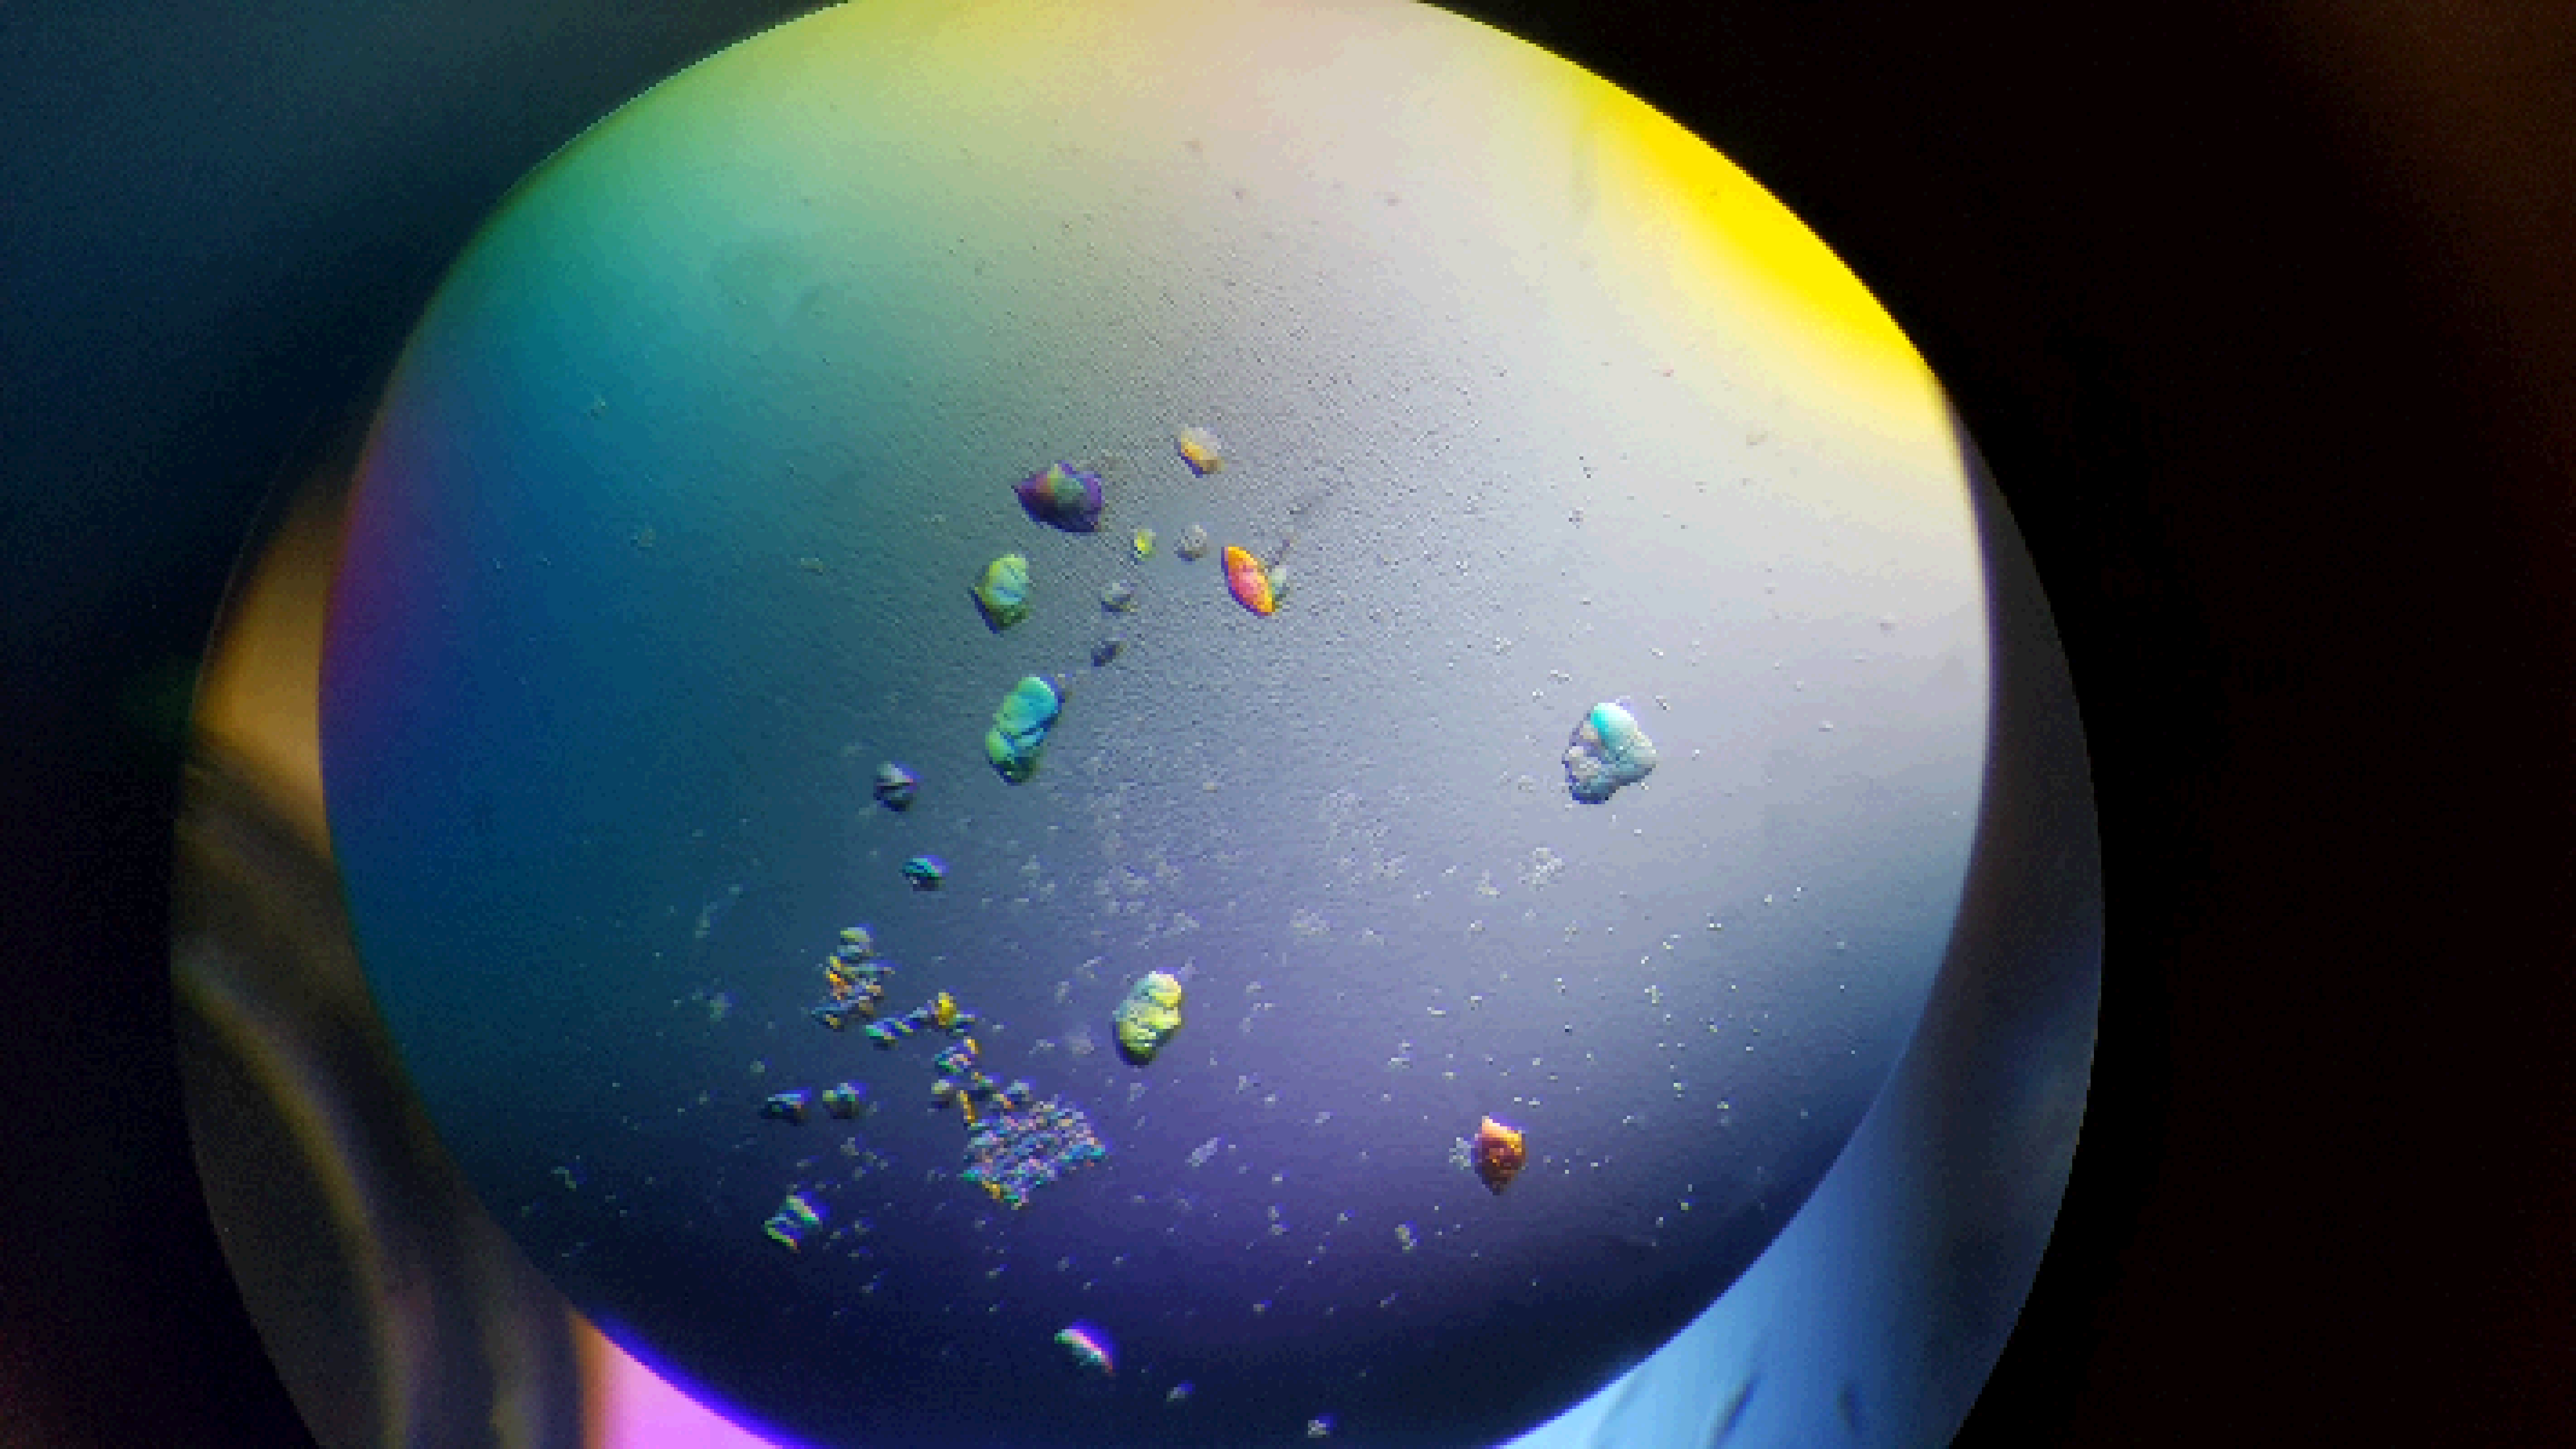
\includegraphics[width=0.45\textwidth, trim={500 50 700 250},clip]{/Users/joehealey/Documents/Warwick/PhD/Thesis/chapters/chapter5/img/20160908_174339.pdf}
	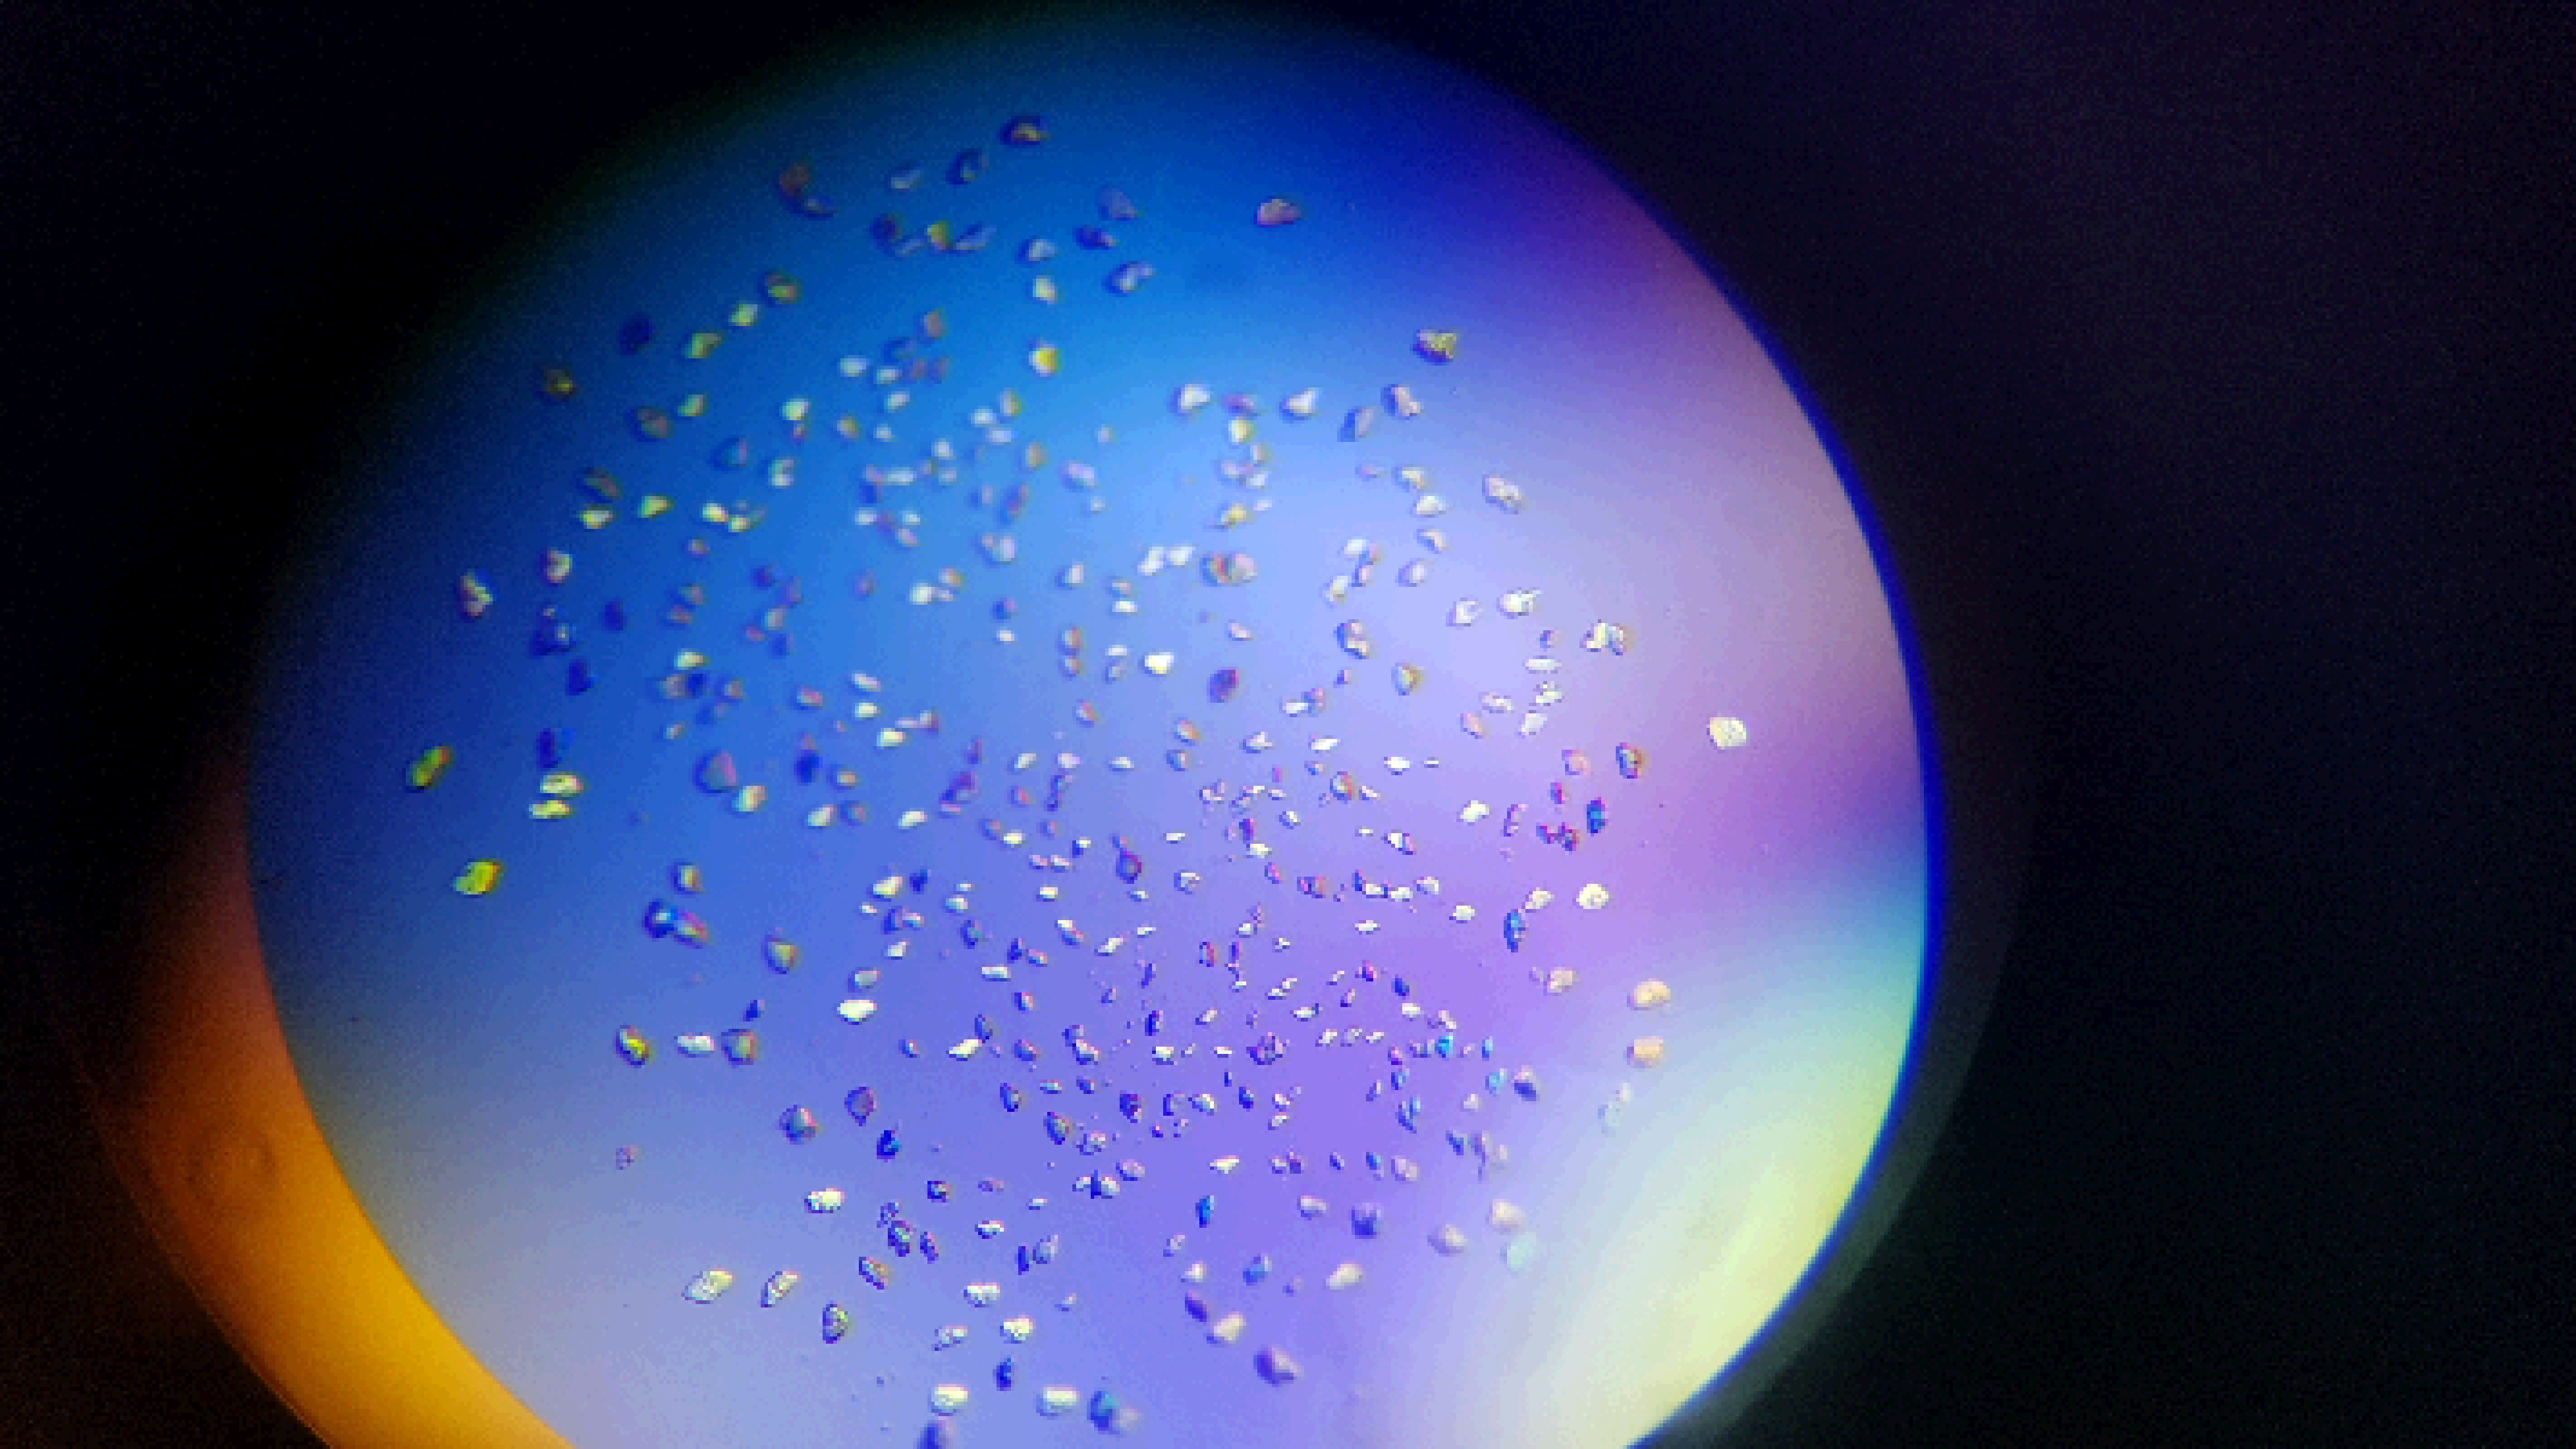
\includegraphics[width=0.45\textwidth, trim={400 50 800 250},clip]{/Users/joehealey/Documents/Warwick/PhD/Thesis/chapters/chapter5/img/20160908_174445.pdf}
	
	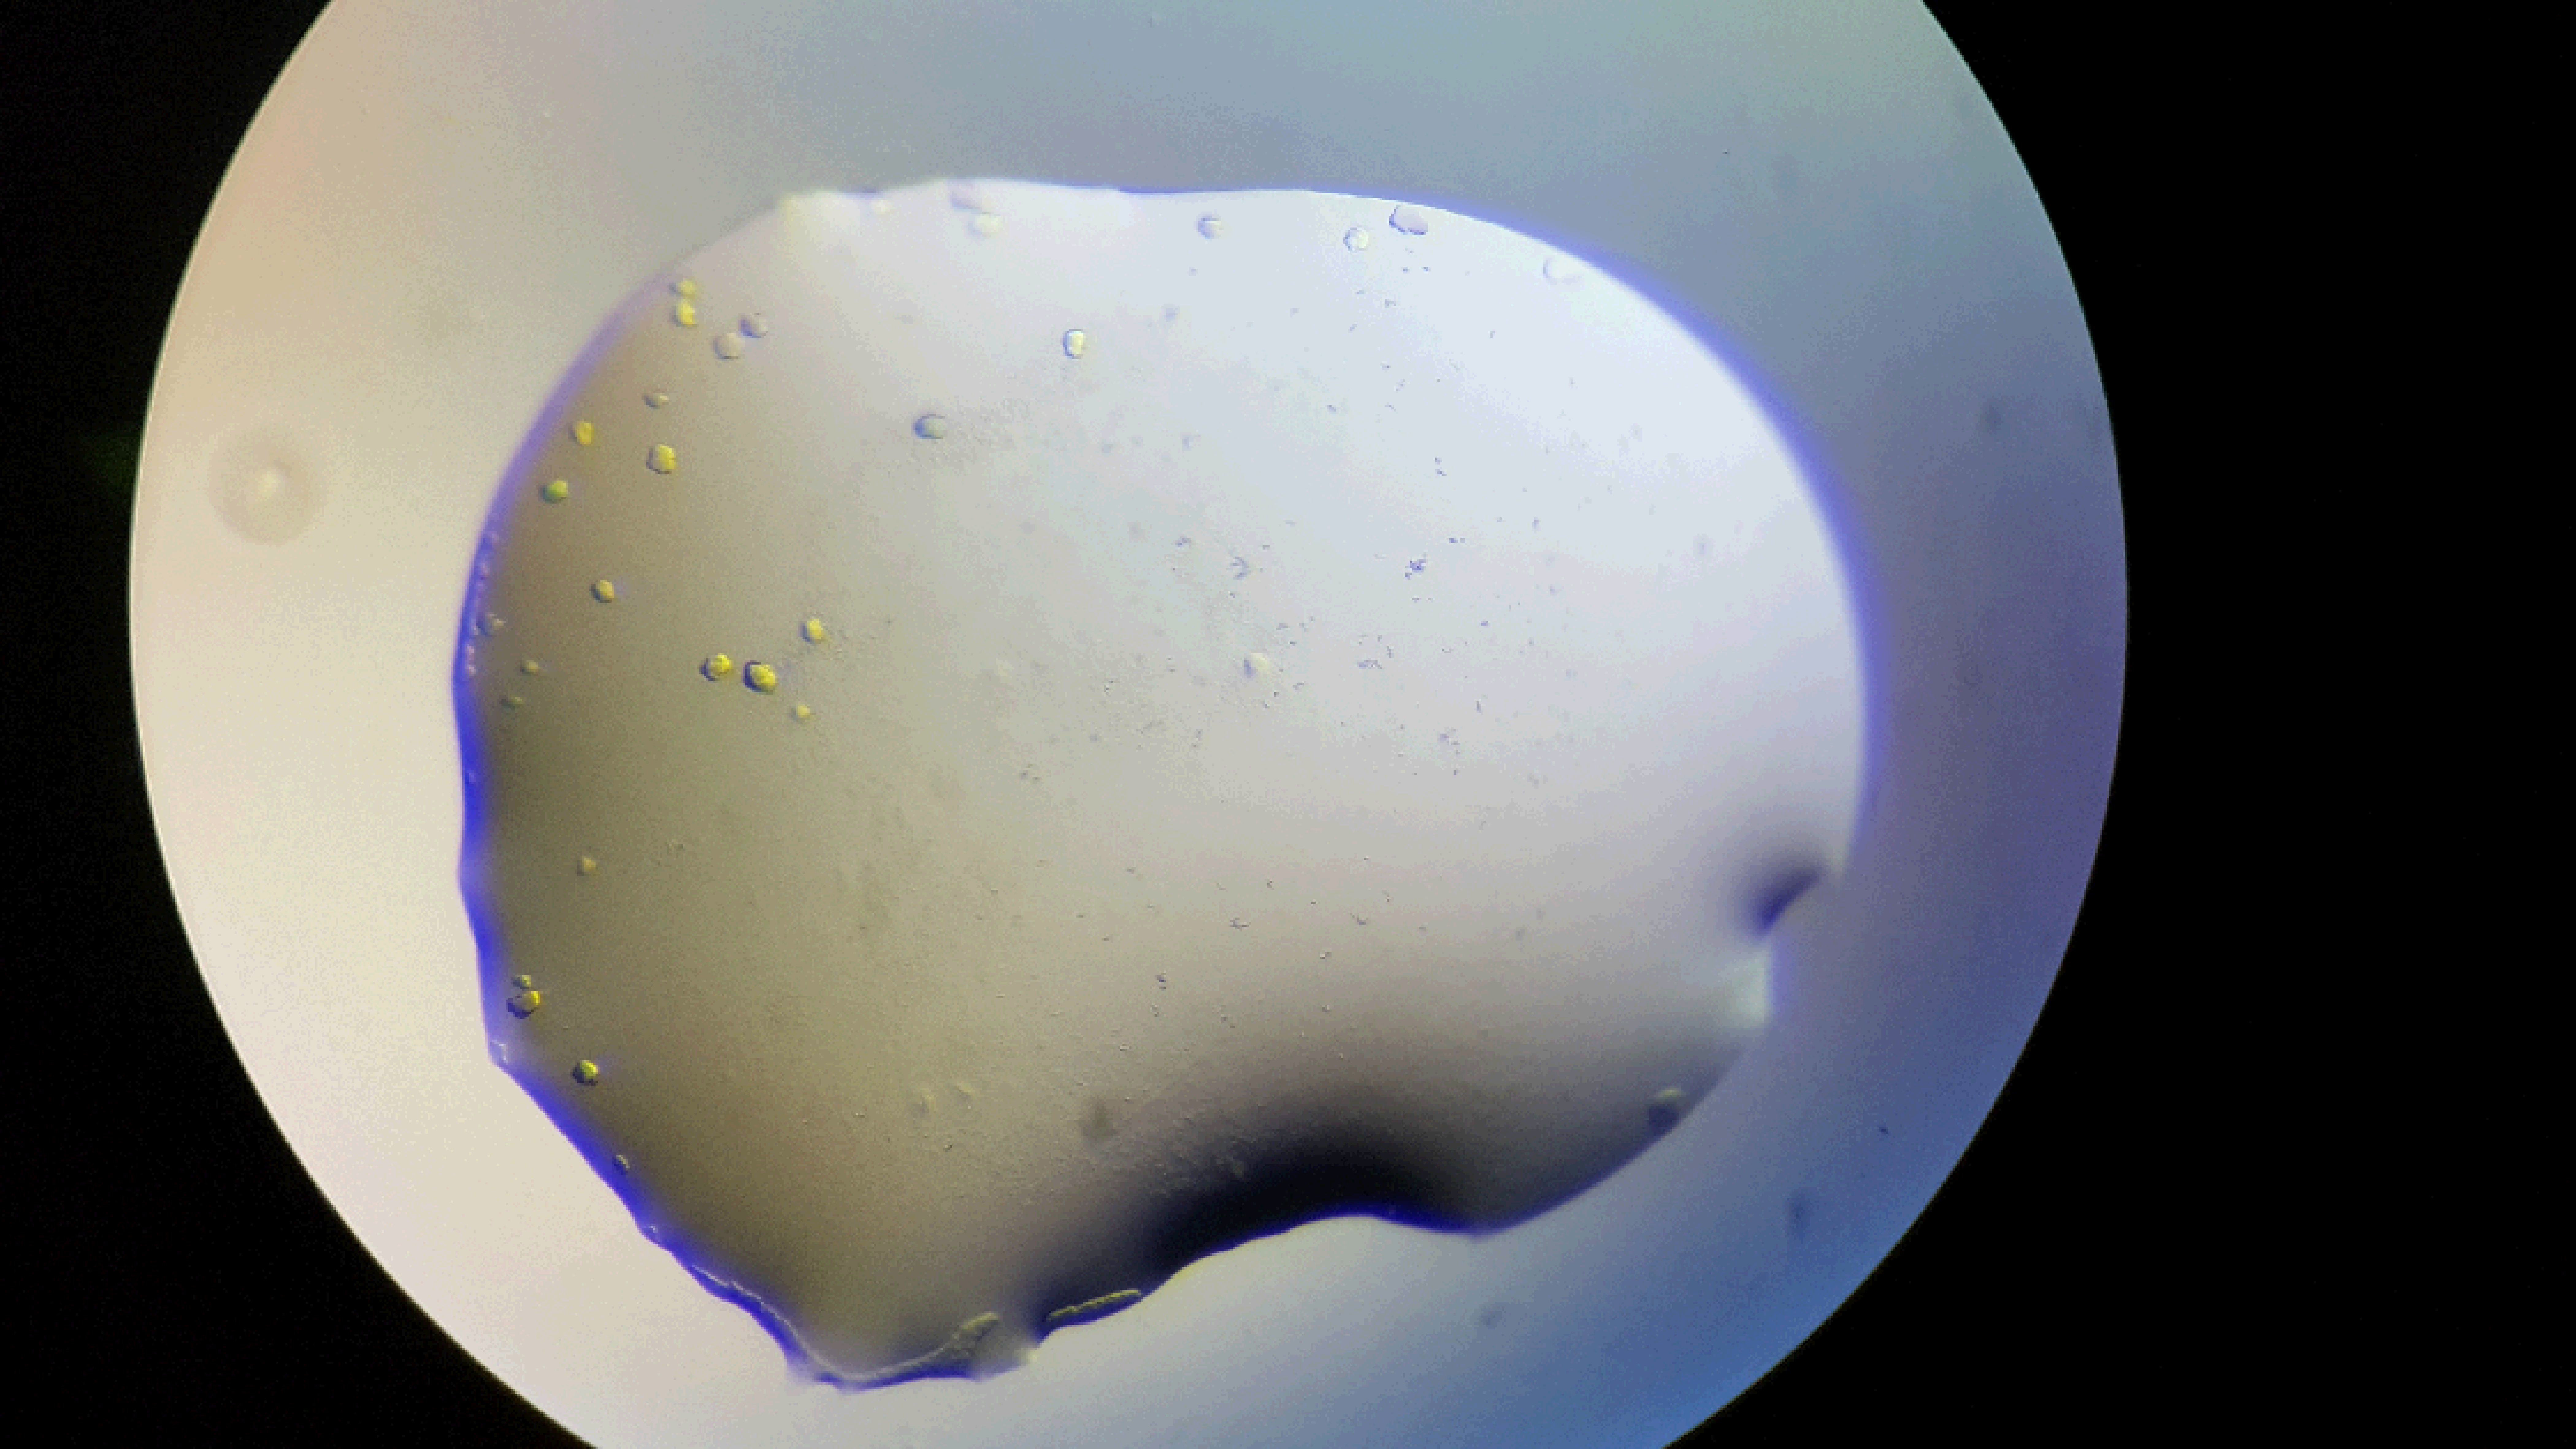
\includegraphics[width=0.45\textwidth, trim={500 50 1000 100},clip]{/Users/joehealey/Documents/Warwick/PhD/Thesis/chapters/chapter5/img/20170429_182707.pdf}
	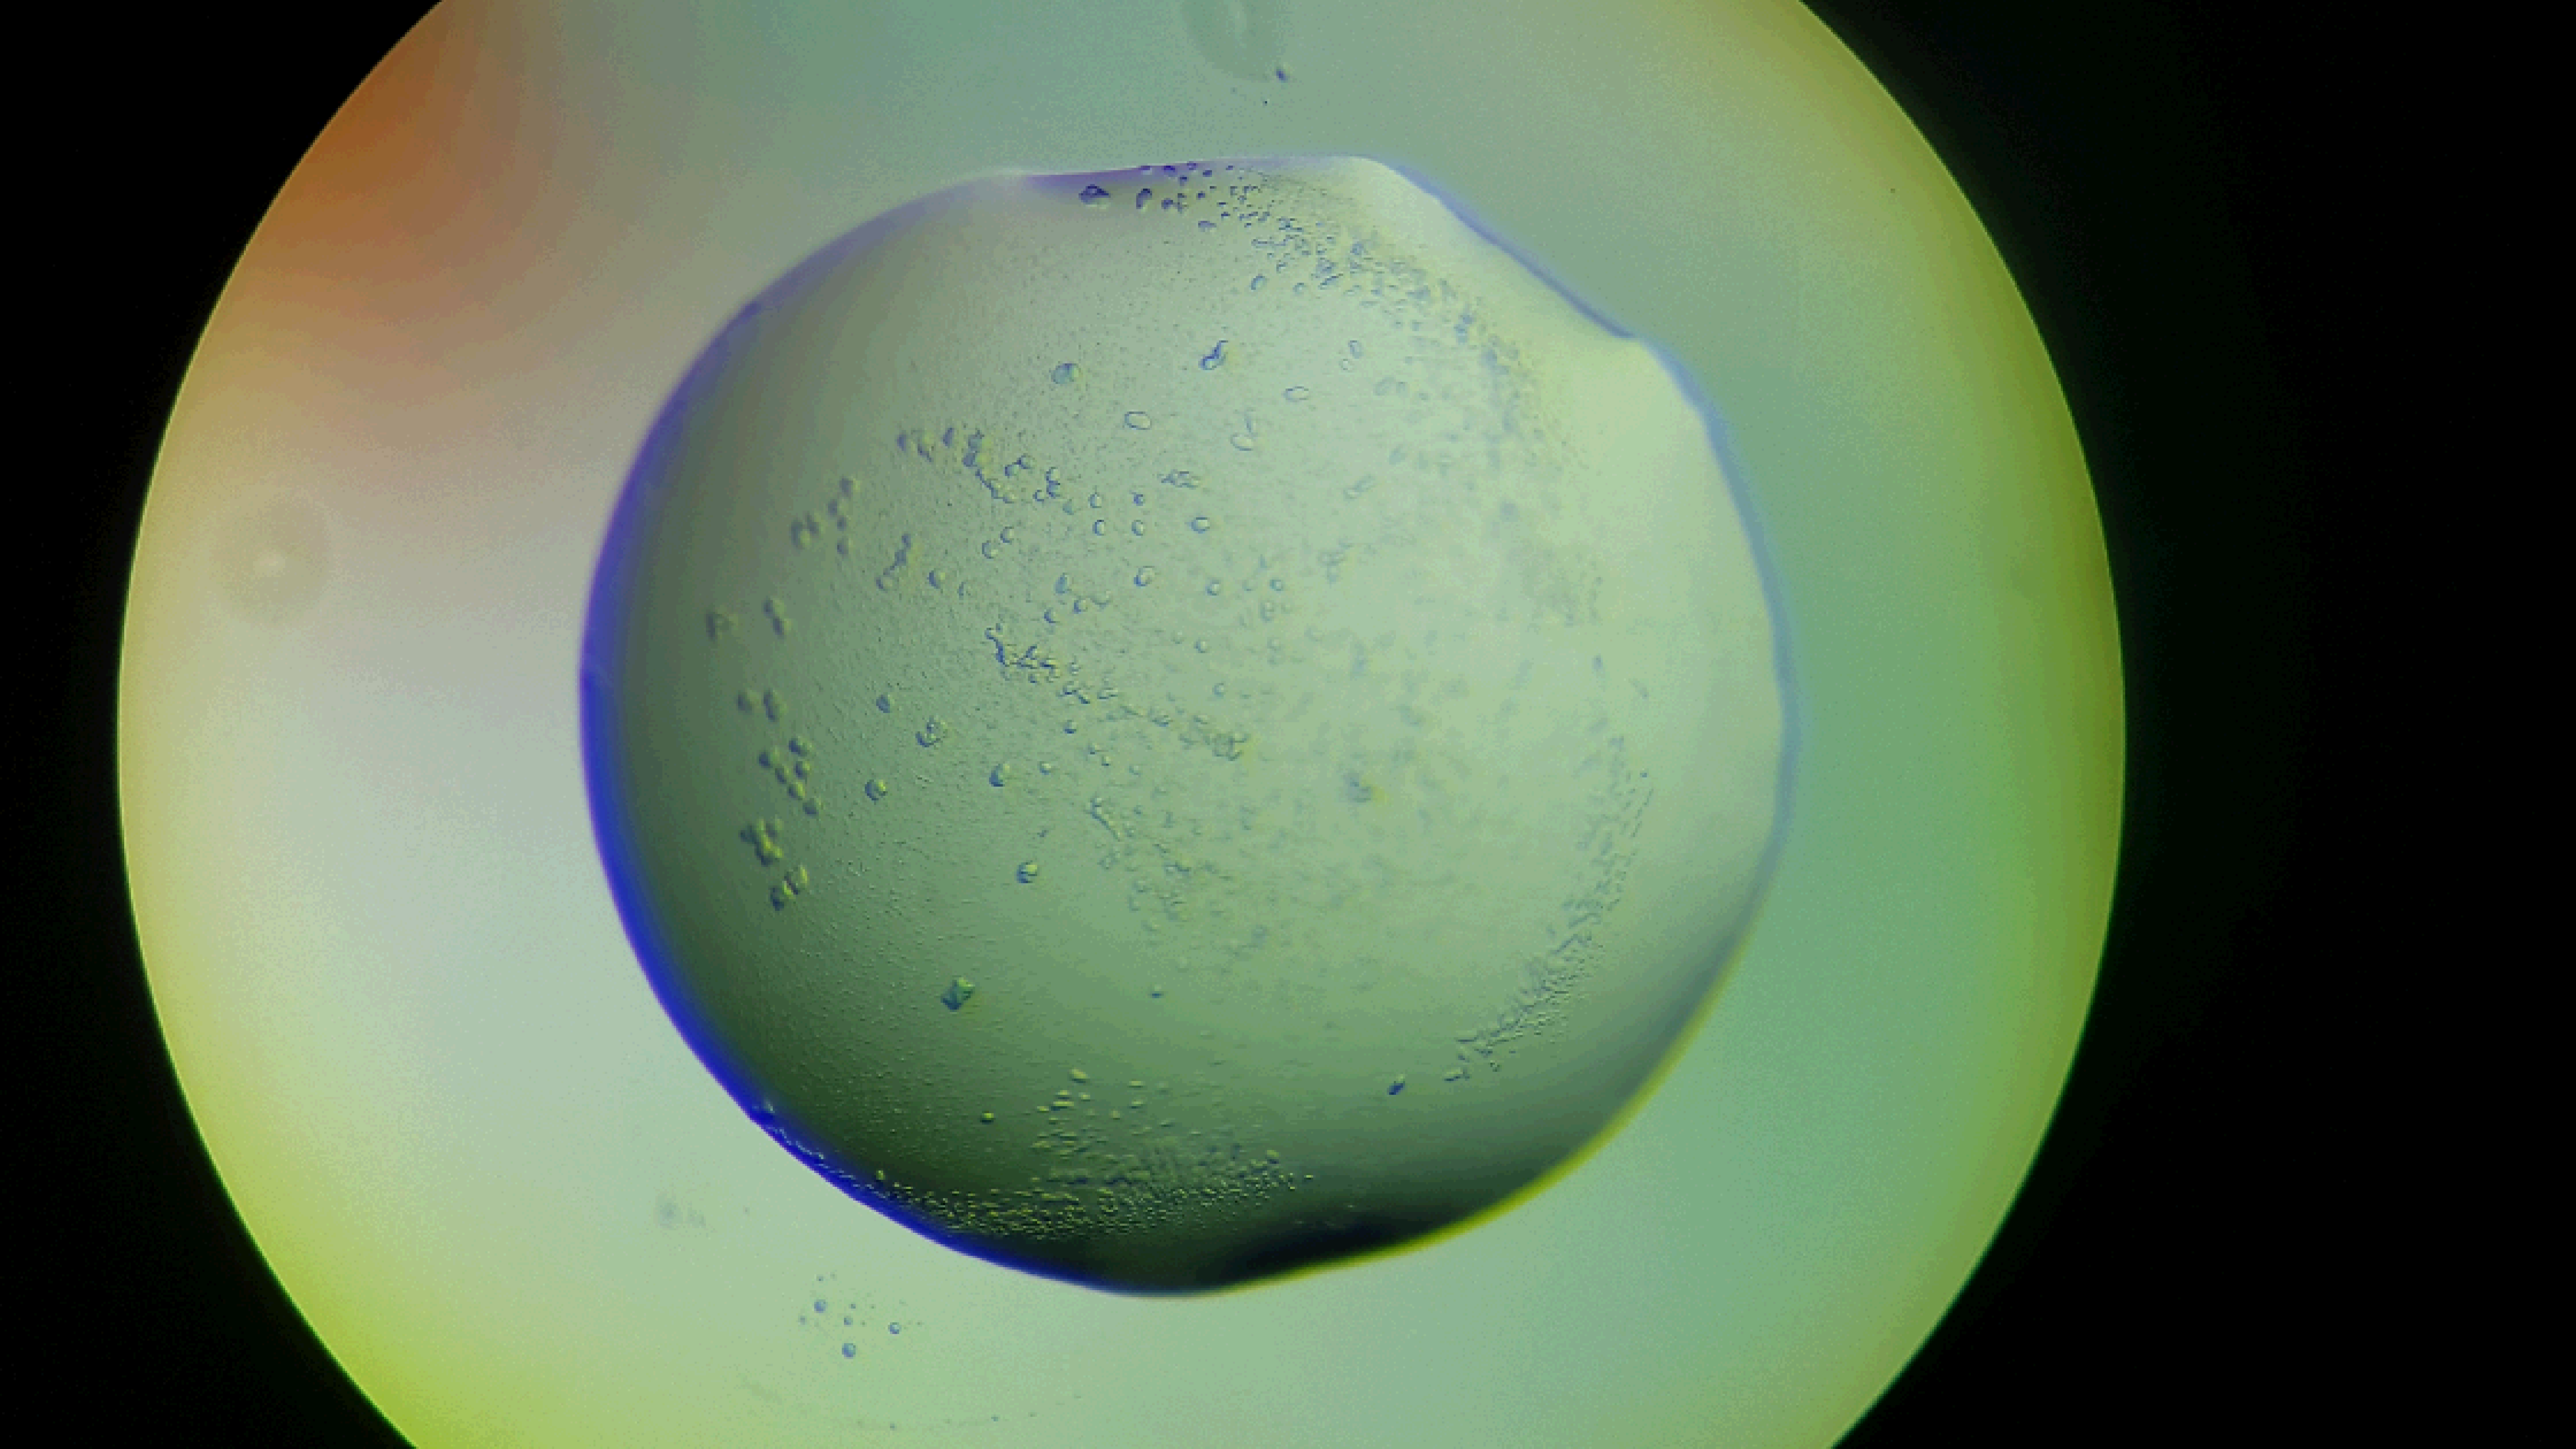
\includegraphics[width=0.45\textwidth, trim={750 250 1050 145},clip]{/Users/joehealey/Documents/Warwick/PhD/Thesis/chapters/chapter5/img/20170429_183352.pdf}
	
	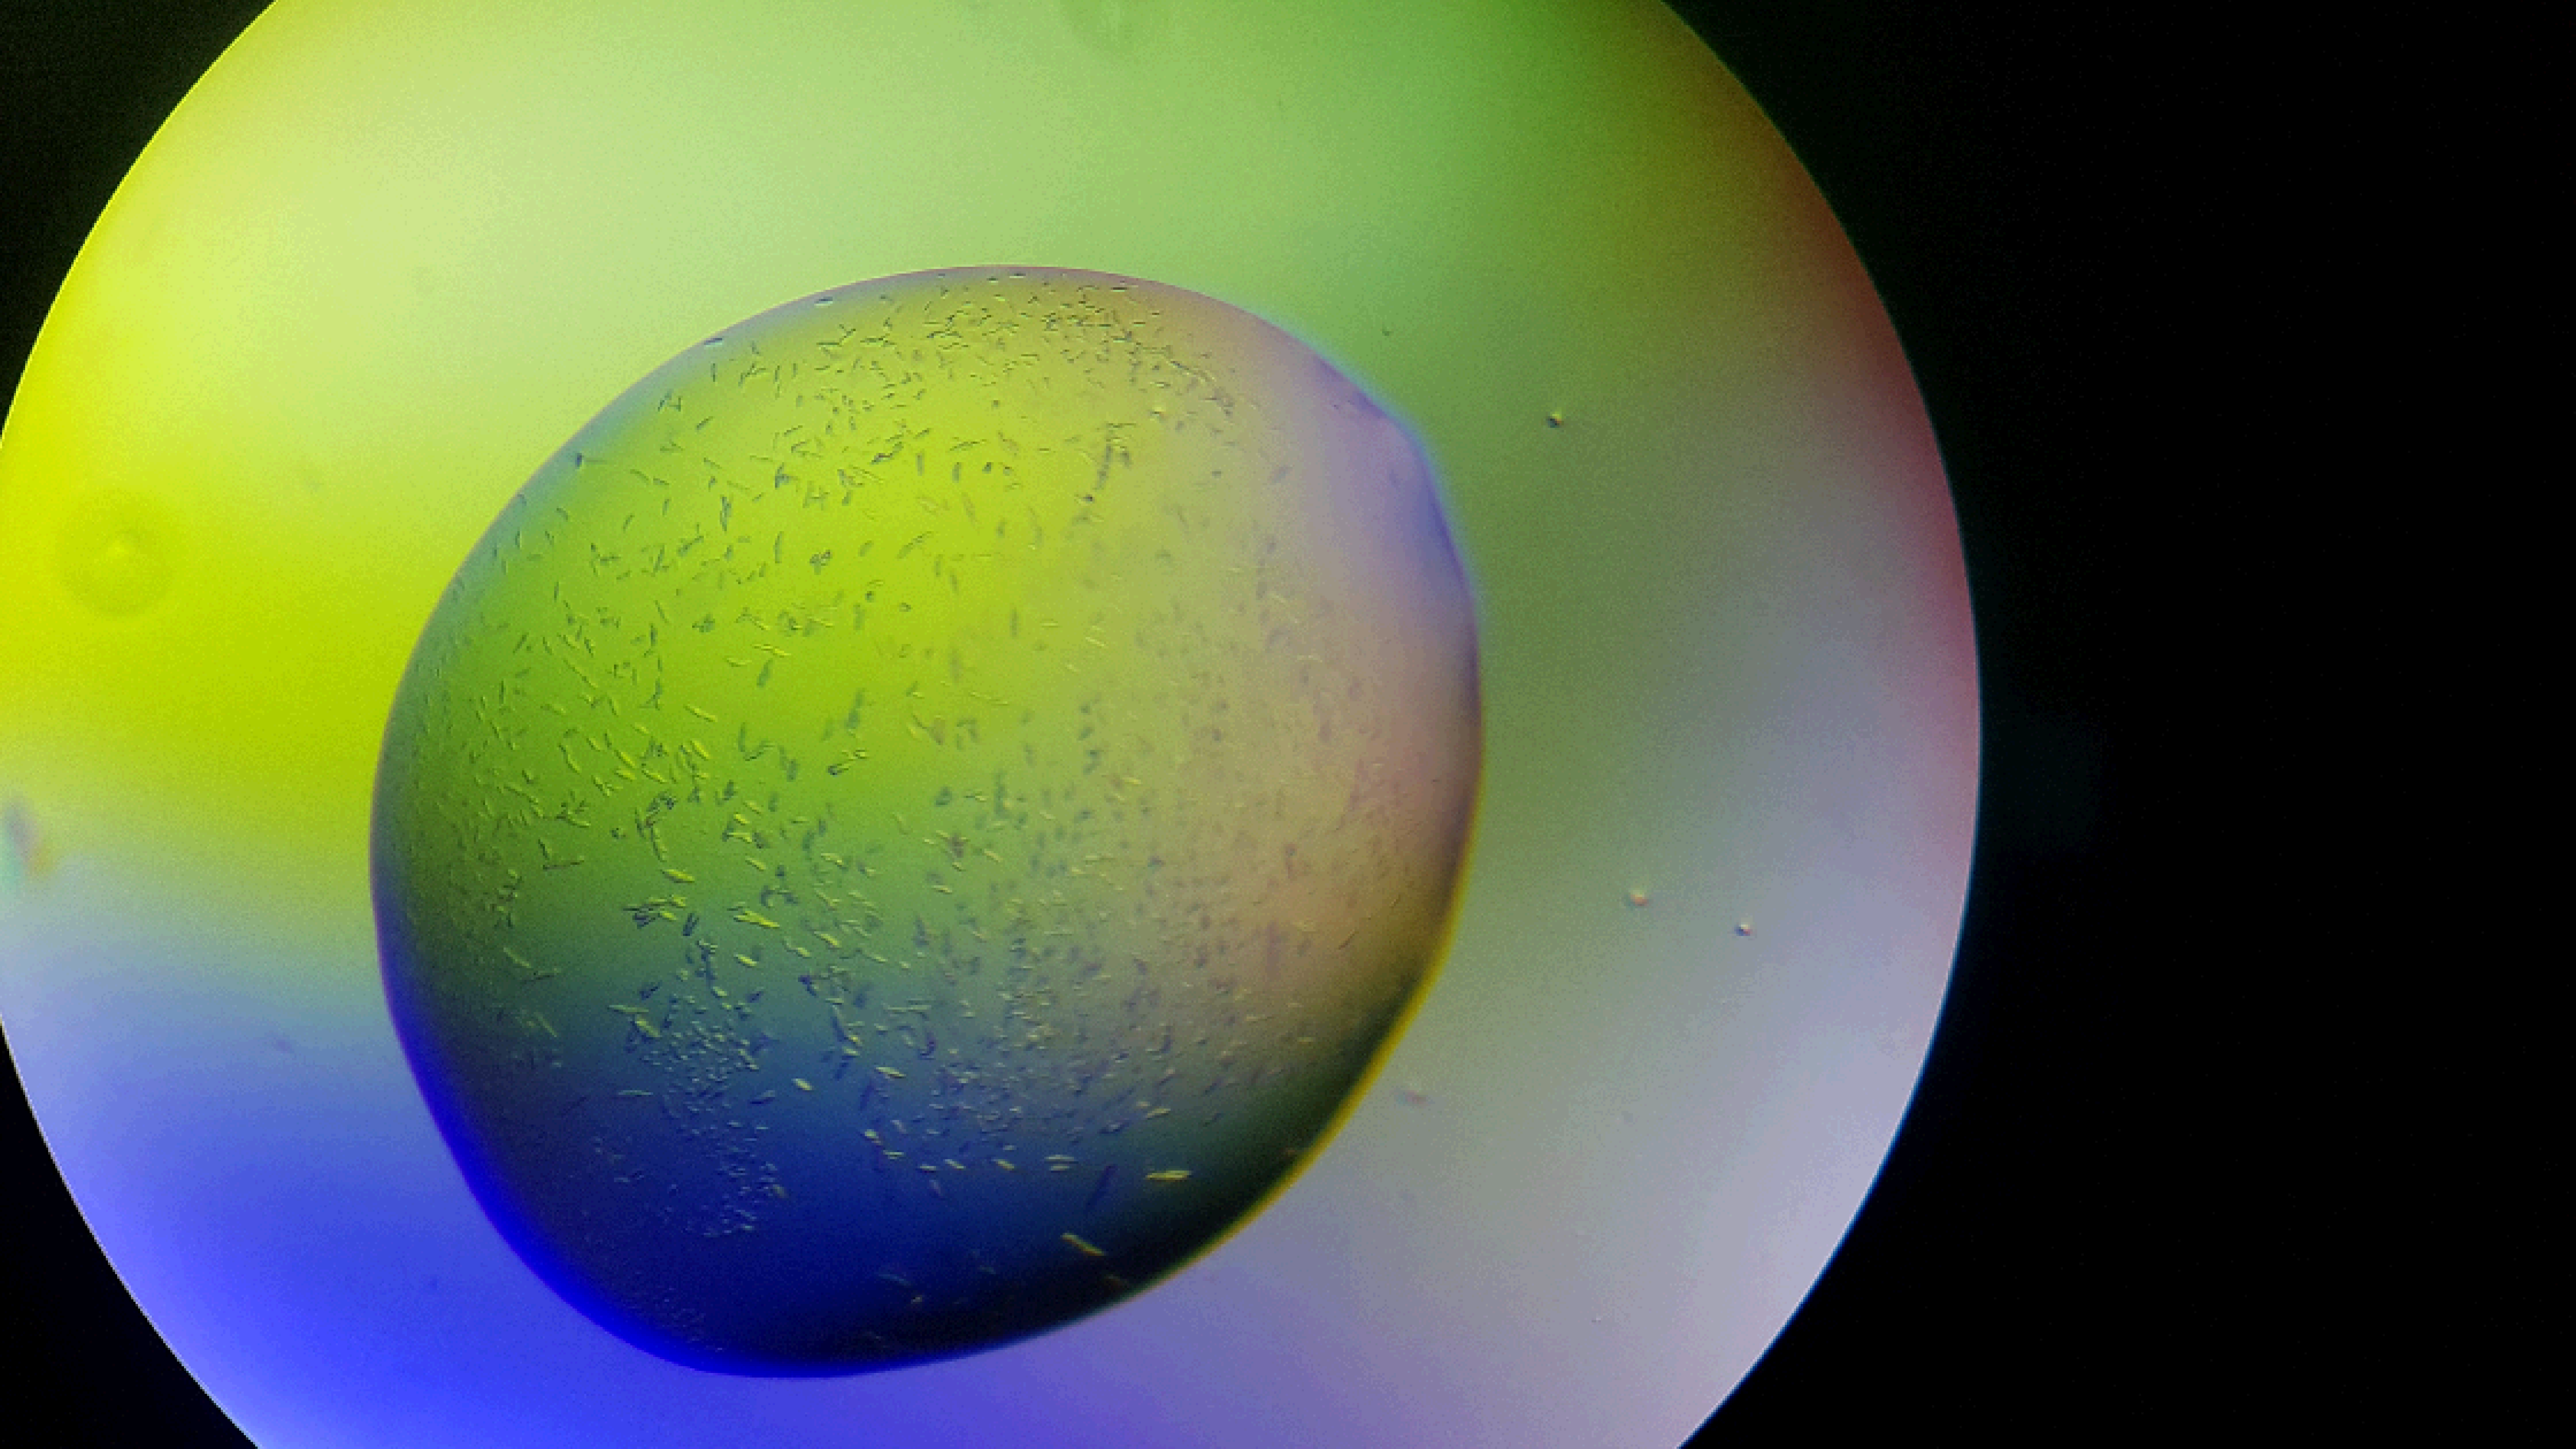
\includegraphics[width=0.45\textwidth, trim={500 350 1500 400},clip]{/Users/joehealey/Documents/Warwick/PhD/Thesis/chapters/chapter5/img/20170429_183451.pdf}
	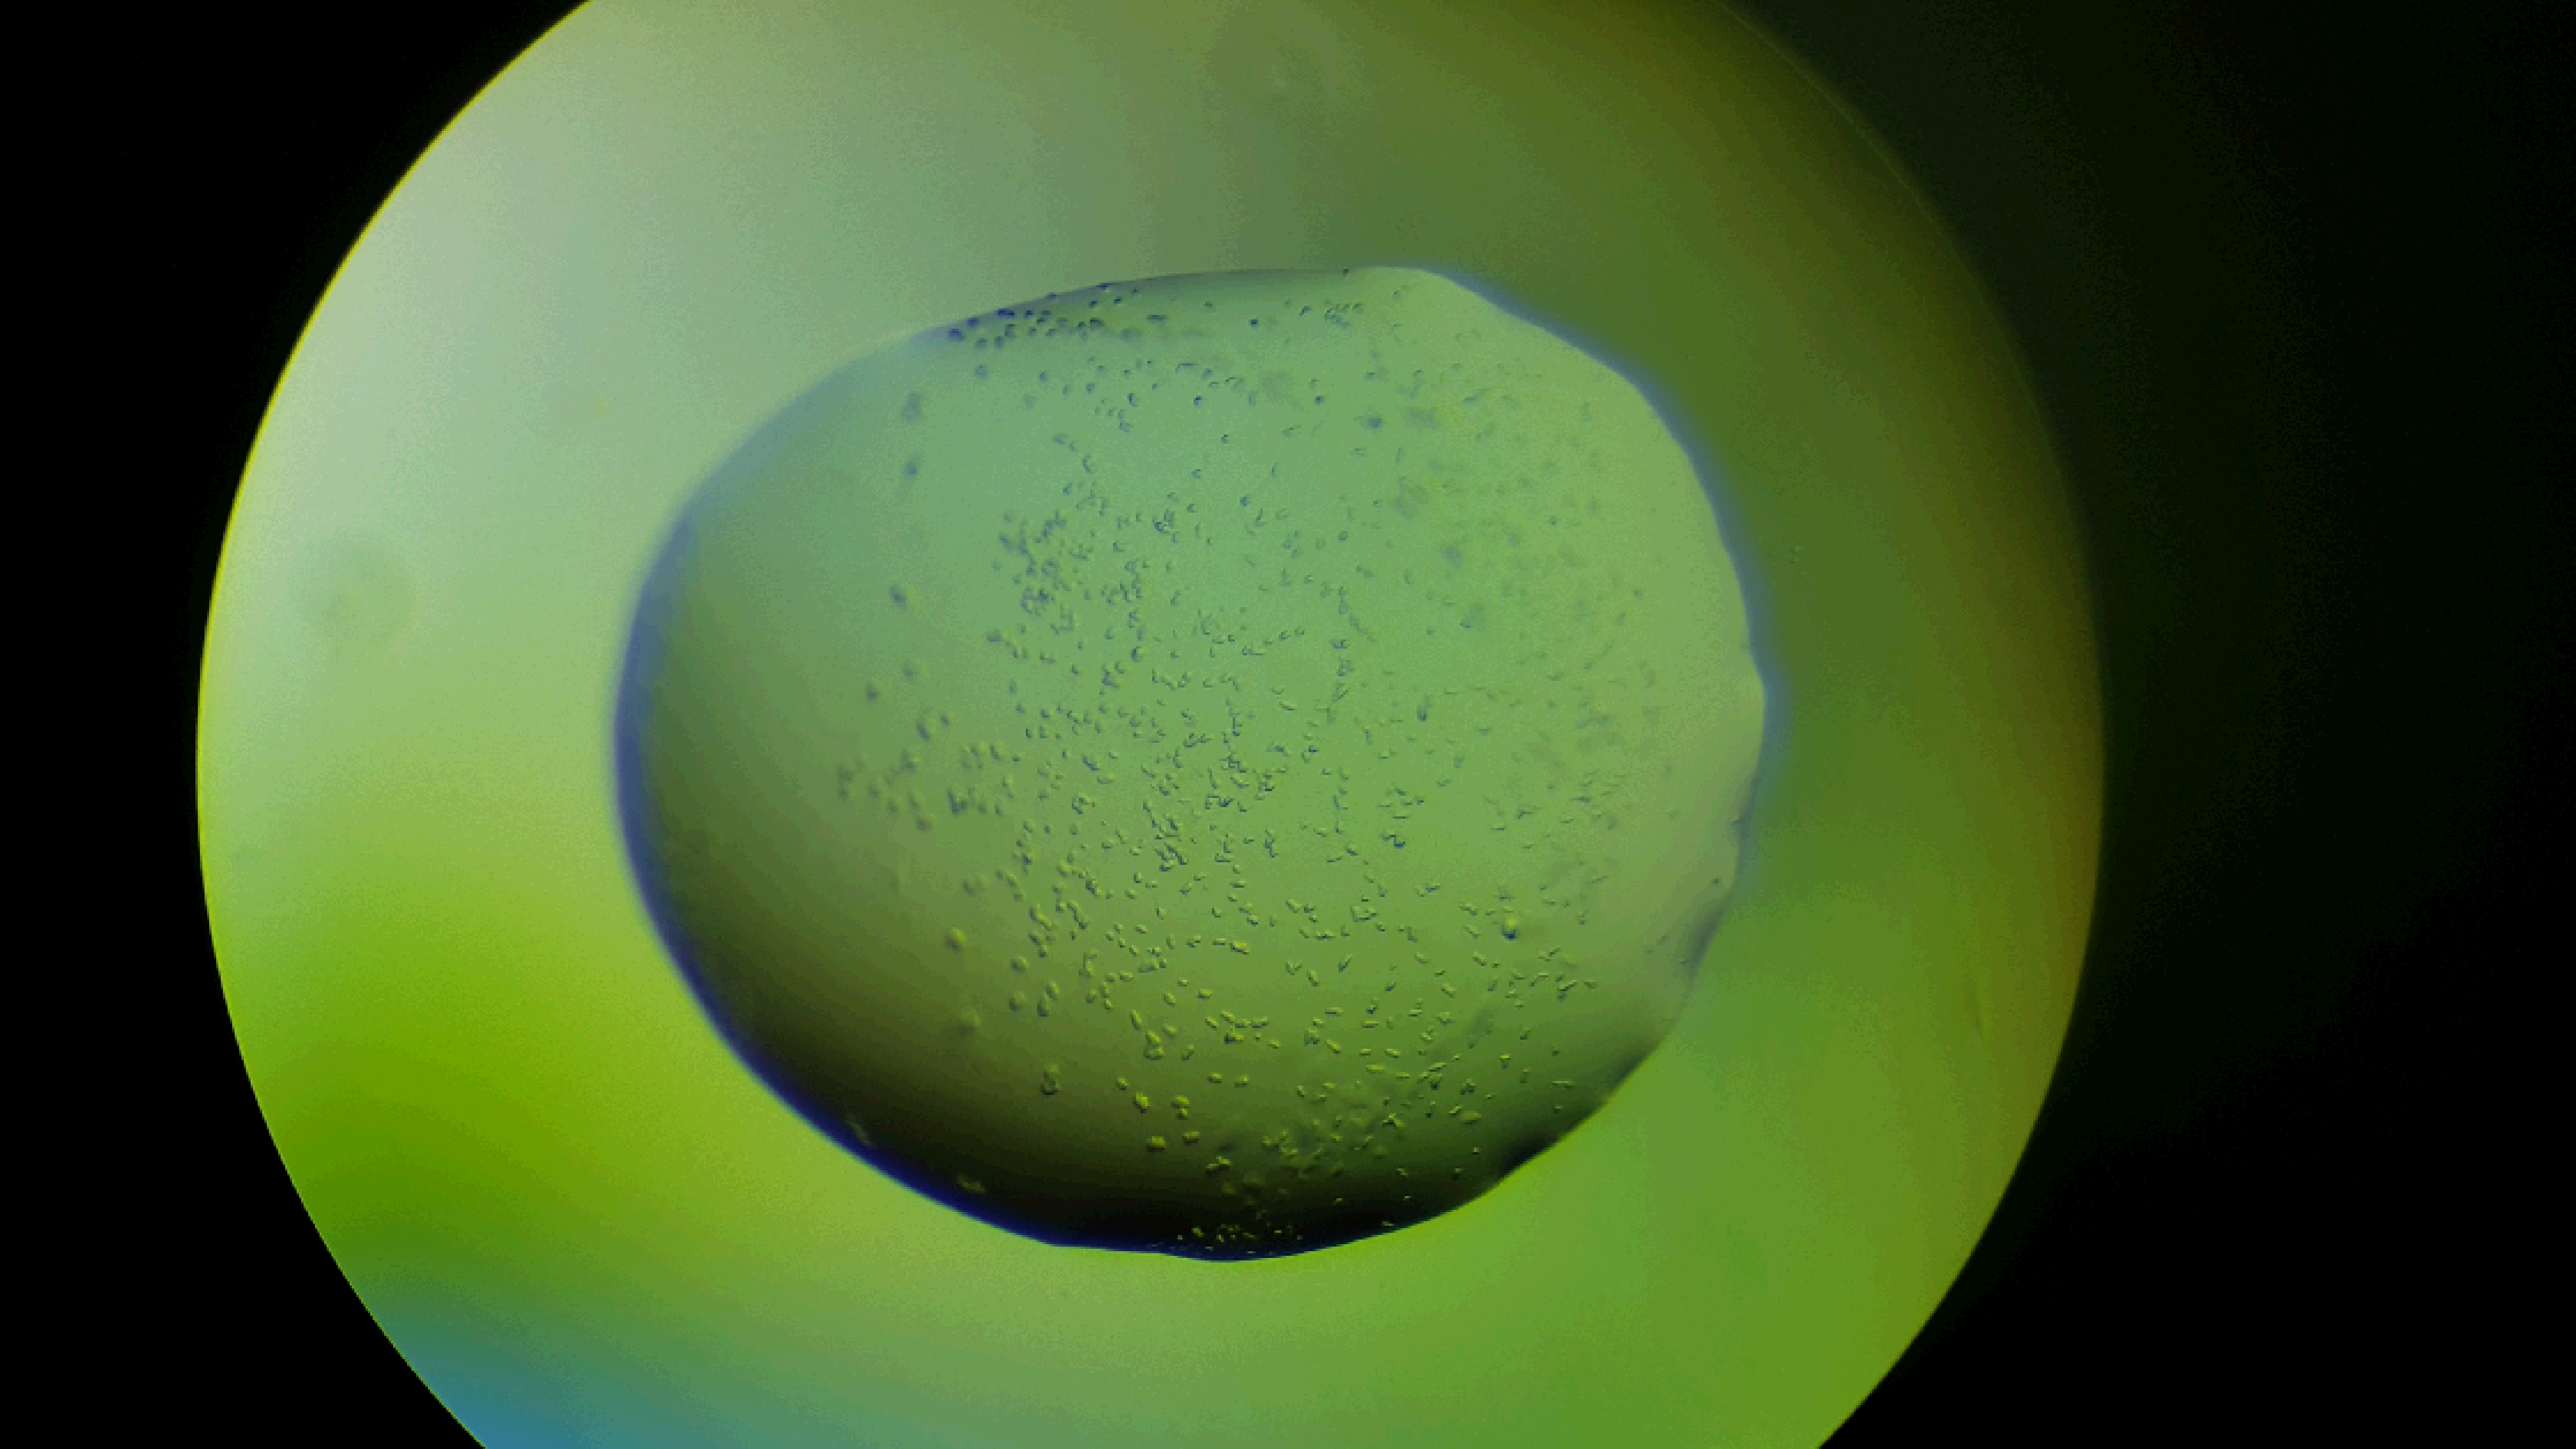
\includegraphics[width=0.45\textwidth, trim={700 350 1100 252},clip]{/Users/joehealey/Documents/Warwick/PhD/Thesis/chapters/chapter5/img/20170429_183740.pdf}
	
	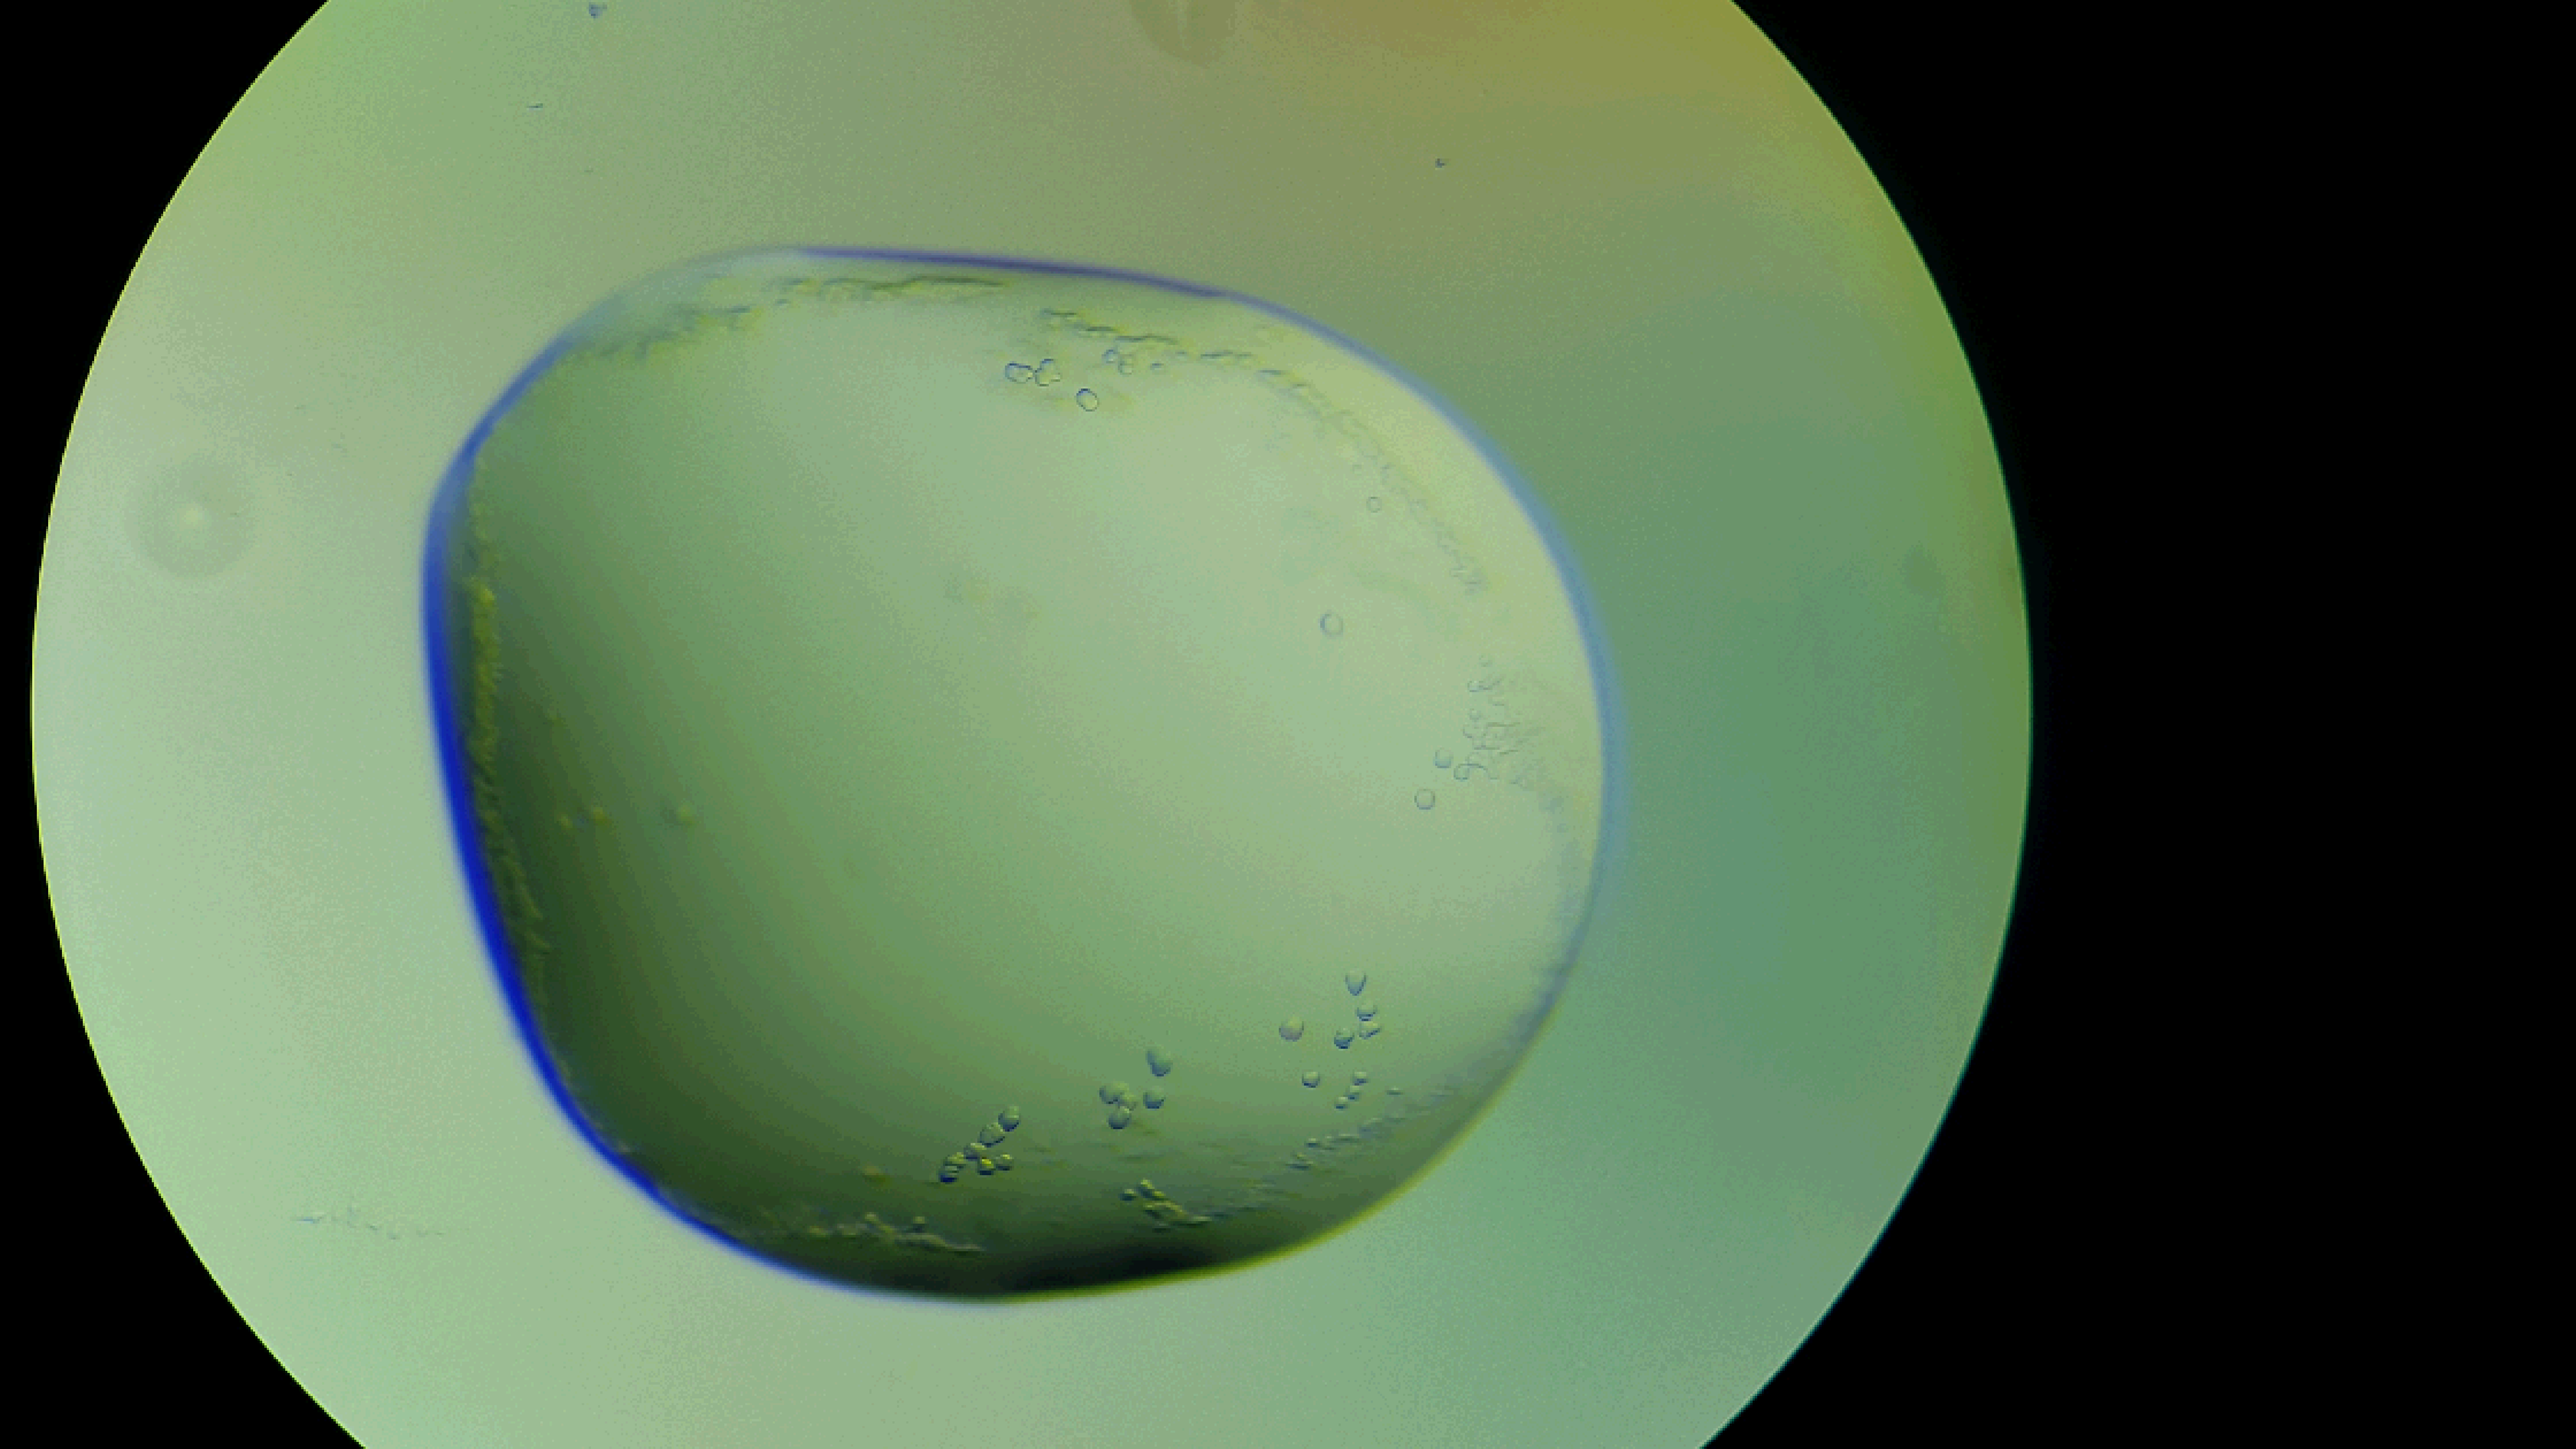
\includegraphics[width=0.45\textwidth, trim={500 250 1200 245},clip]{/Users/joehealey/Documents/Warwick/PhD/Thesis/chapters/chapter5/img/20170429_185249.pdf}
	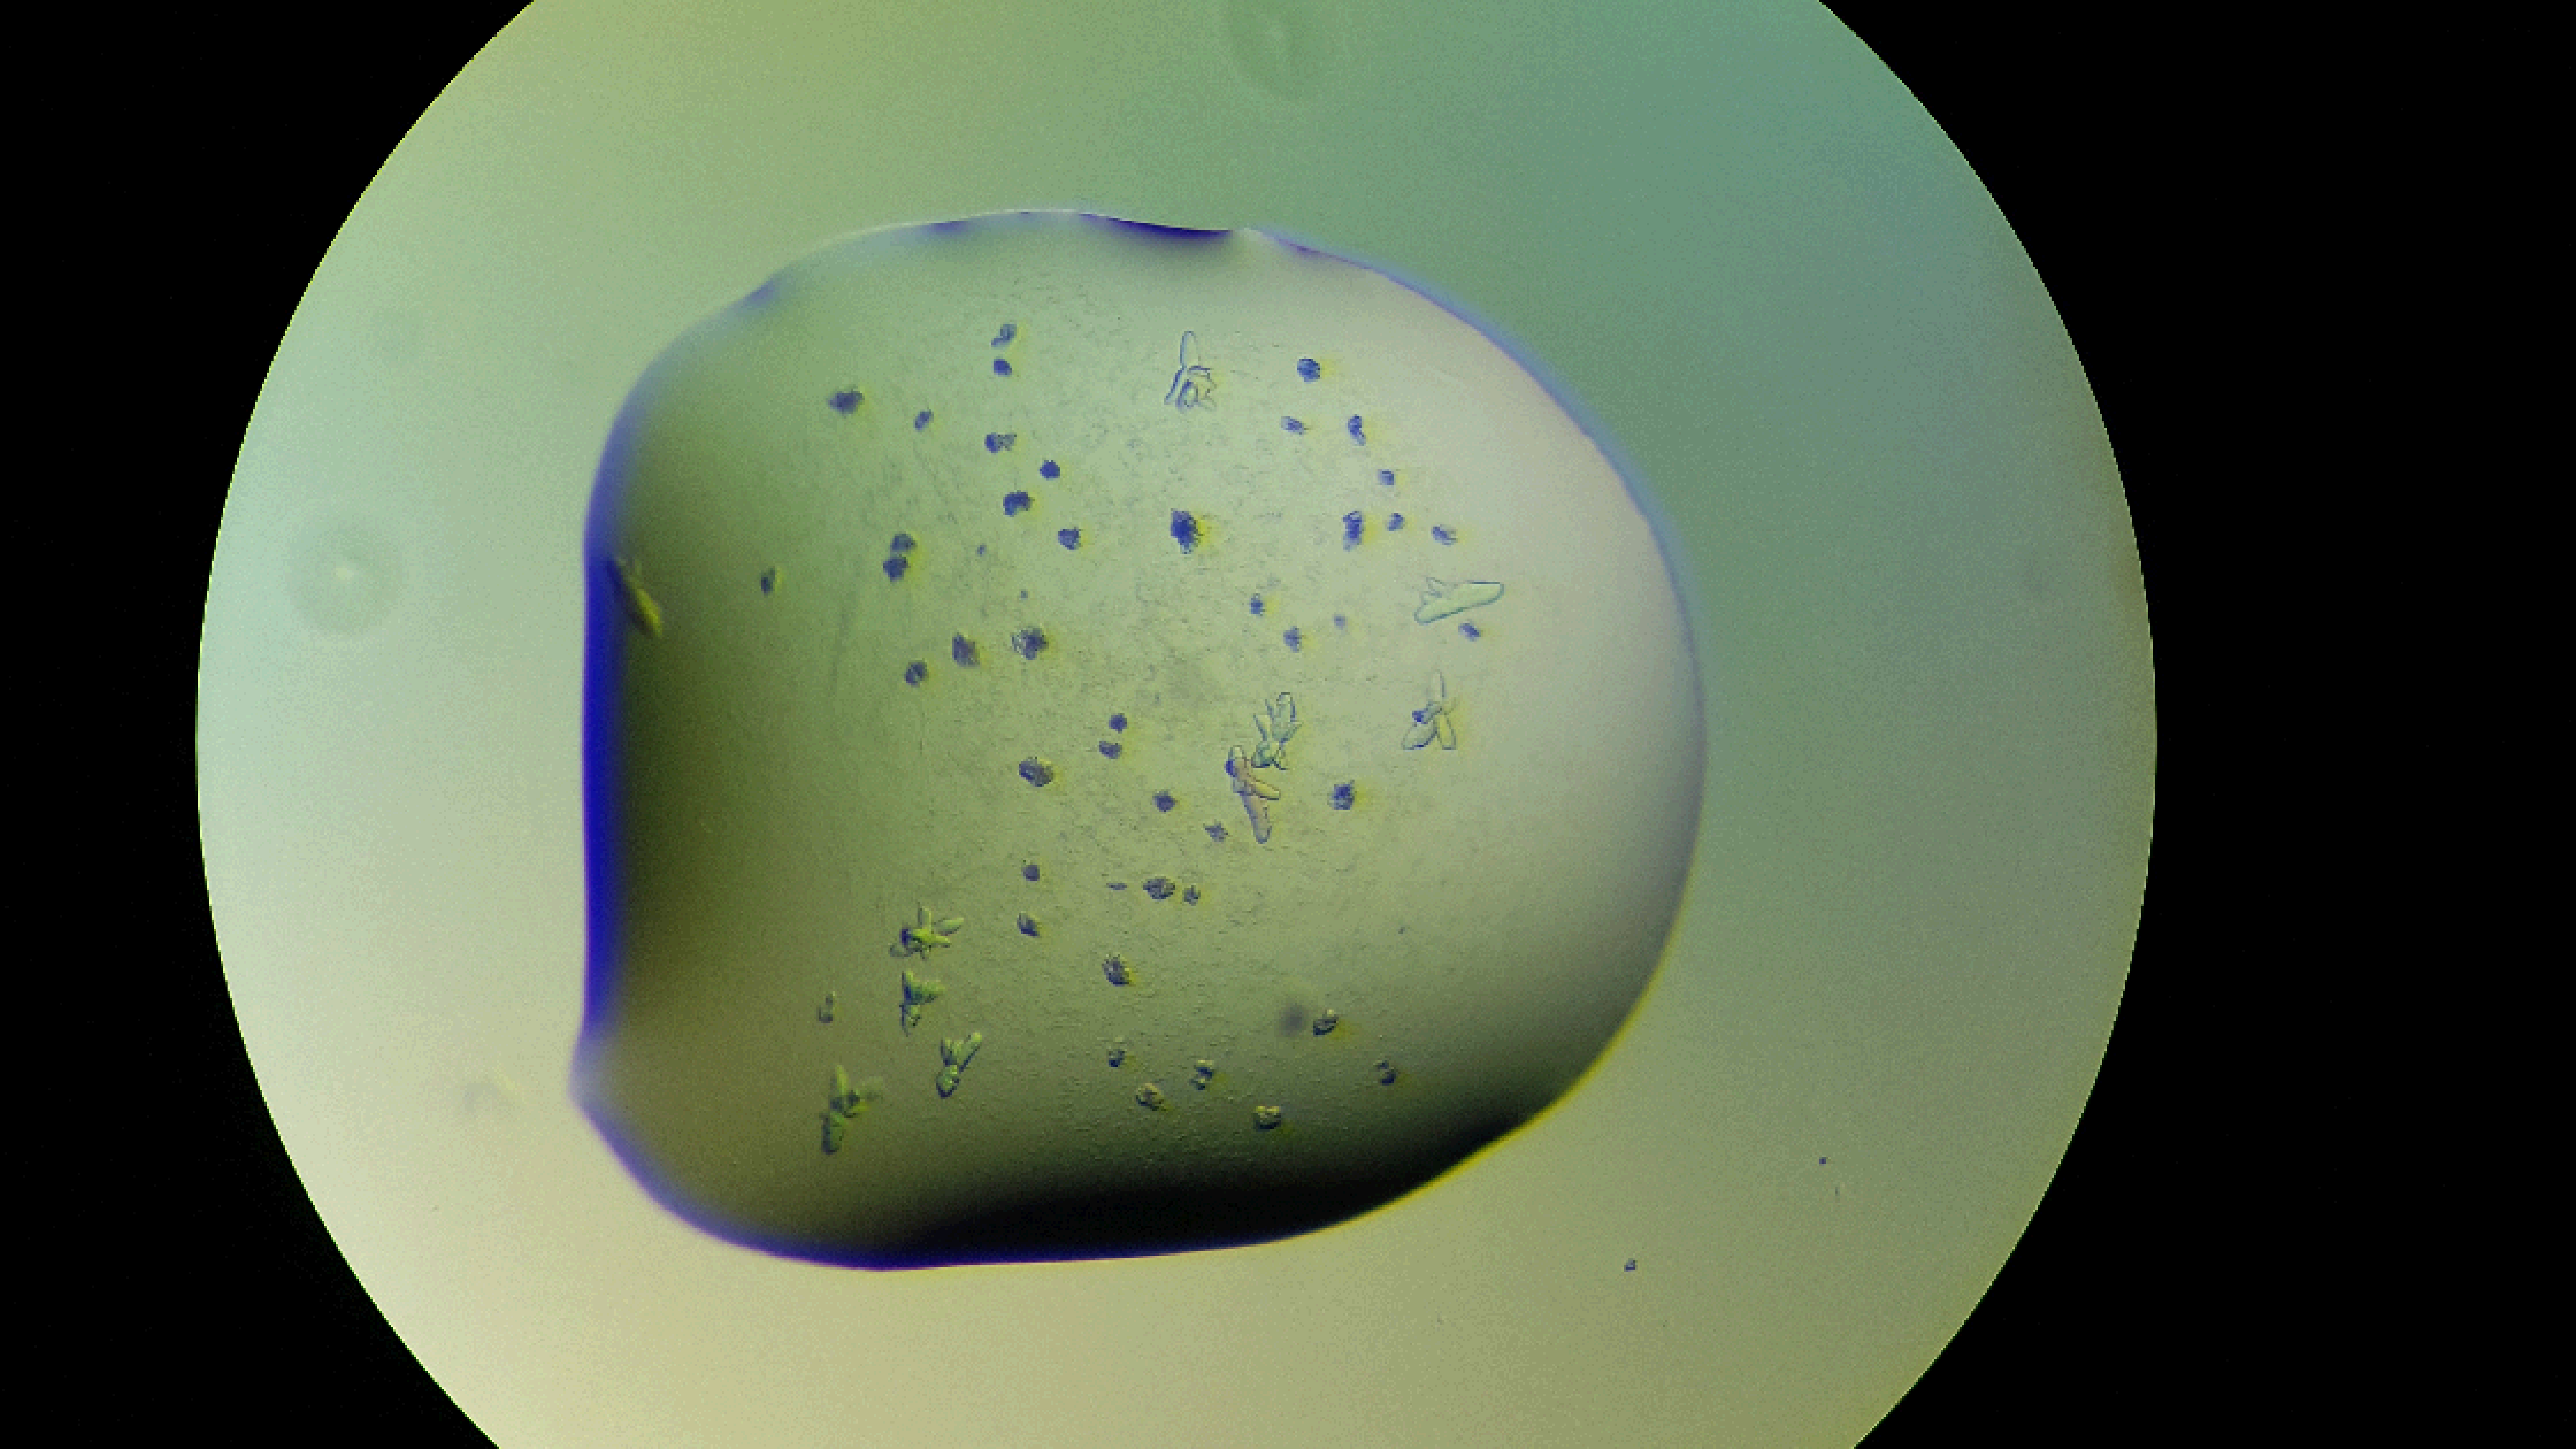
\includegraphics[width=0.45\textwidth, trim={700 340 1250 345},clip]{/Users/joehealey/Documents/Warwick/PhD/Thesis/chapters/chapter5/img/20170429_185734.pdf}

	\captionsetup{singlelinecheck=off, justification=justified, font=footnotesize, aboveskip=10pt}
	\caption[Crystal images]{\textsc{\normalsize A selection of lumt13 crystal morphologies.}\vspace{0.1cm} \newline A selection of the crystal morphologies obtained from crystal screening with lumt13 and the Mosquito robot, corresponding to some of the conditions in \vref{crystalconditionstable}.}
	\label{crystals}
\end{figure}

\clearpage

\subsection{Finding Binding Partners for Tail Fibre Proteins}
A key long term aim is to be able to specifically identify the tissues and the molecular partners that the tail fibres are preferentially binding to. A rationale for the diversity seen within the tail fibre proteins is that they may have diverged to target specific cell or tissue types as part of the PVCs role in virulence. Cloning and purifying the tail fibres in isolation from the rest of the PVCs was done in order to enable a suite of downstream bioassays without the complications of the large PVC component itself. The polyhistidine tags that the PVC tail fibres exhibit from cloning are useful `functional handles', and several assays were designed around their use. This work was conducted in collaboration with another PhD student, who was responsible for devising the methods, so only the preliminary data obtained from these assays and their conceptual basis will be discussed. Nanoparticle conjugation of proteins is a well studied process however, and the reader is directed to \cite{Sperling2010} and \cite{Hainfeld1999} for a good review and discussion of the mechanism.


\subsubsection{Iron Nanoparticle Protein Pulldowns}
Magnetic (iron) nanoparticle (commonly and commercially known as ``Dynabeads") pull down protocols were developed, such that the tail fibres could be incubated with whole protein extracts from tissues of interest to broadly identify candidate binding partners. Briefly, these assays simply required conjugation of the polyhistidine tagged tail fibres to iron nanoparticles which were coated in the chelator nitrilotriacetic acid (NTA), which in turn coordinates Nickel (see \vref{nanoparticle}). This is the same chemistry as that used in the IMAC purification process.

After incubation of the nanoparticle-tailfibre complex with cellular lysates from mammalian cell lines, the particles are pulled from solution magnetically. The particle complexes can then be washed and have the nanoparticles eluted with imidazole (in the same way as IMAC again). Once the tail fibres and any proteins they have bound are free of the iron nanoparticles, they are processed via Orbitrap mass spectrometry to identify peptides. Proteins which have bound to the tail fibres should be enriched in the pulldown samples. Candidates from preliminary studies with the PVClumt13 tail fibres incubated with lysates from A549 lung epithelial carcinoma cell lines are shown in \vref{pulldowncandidates}. These candidates were shown as statistically significantly enriched in peptide numbers matching to these proteins between sample and controls. They have also been filtered to remove likely spurious or uninformative hits (i.e., common contaminants have been discarded, and only proteins with plausible cell surface localisation have been retained). These pulldown studies are still preliminary; as more tail fibres can be tested with more cell lines, patterns in the binding activity of the tail fibres may begin to emerge, though some promising results are detected.


\begin{figure}[h]
\centering
    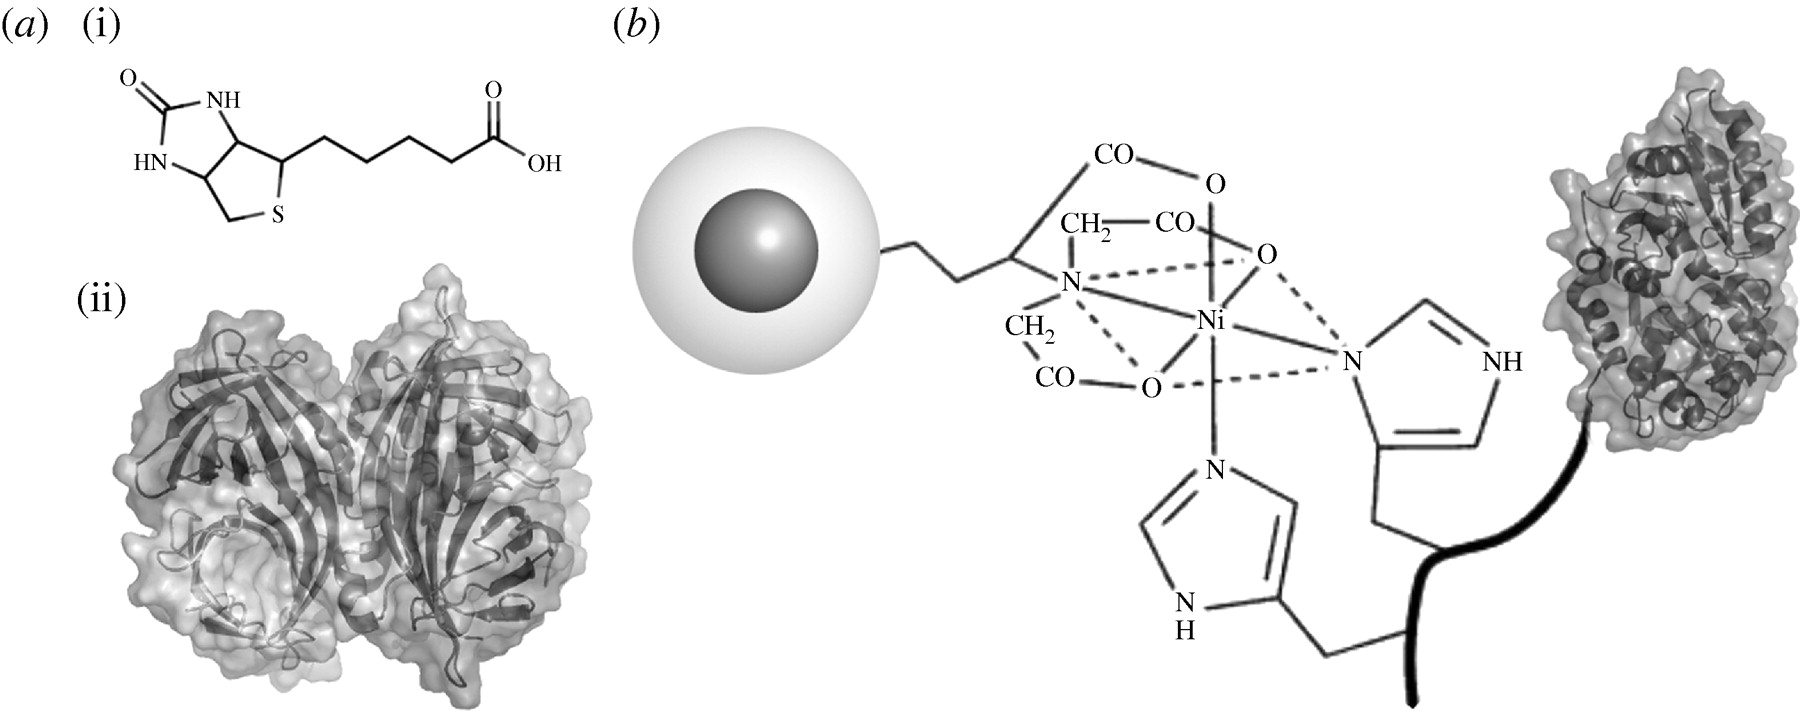
\includegraphics[width=0.5\textwidth, trim={600 0 0 50}, clip]{nanoparticle_hd.png}
	\captionsetup{singlelinecheck=off, justification=justified, font=footnotesize, aboveskip=10pt}
	\caption[Dynabead particle interactions]{\textsc{\normalsize Nanoparticle-Ni-NTA interactions with polyhistidine tracts.}\vspace{0.1cm} \newline A structural and illustrative diagram of the interaction between metal nanoparticles, Nickel nitrolotriacetic acid chelating coordination groups, and the polyhistidine tracts of a target protein. Image adapted and reproduced from \cite{Sperling2010}, which in turn is adapted from \cite{Hainfeld1999}.}
\label{nanoparticle}
\end{figure}


\clearpage
\footnotesize
\captionsetup{singlelinecheck=off, justification=justified, font=footnotesize}
\rowcolors{1}{gray!20}{white}
\begin{tabularx}{\textwidth}{l l l Z}
\hiderowcolors
\caption[Pulldown candidates identified by mass spectrometry]{\textsc{\normalsize Preliminary candidate proteins enriched in tail fibre Dynabead pulldowns.} \vspace{-0.2cm} \newline This table shows the enriched candidate binding partners from PVClumt13 binding studies. The dataset has been filtered to remove likely contaminant proteins, and to retain only statistically significant, and likely cell surface markers or other proteins with plausible localisations so as to be physiologically relevant to the role of the tail fibres.}
\label{pulldowncandidates}\\
%
Protein & Gene Name & Localisation & Putative Role \\
\hline\hline
\showrowcolors

Protein FAM184A  & FAM184A   & Cell surface/extracellular & Unknown function. \\
Lipocalin-1      & LCN1      & Cell surface/extracellular & Binds a wide range of ligands.\\
Lactotransferrin & LTF       & Nuclear/cell surface/extracellular & Among many functions, LTF promotes binding of species C Adenoviruses to epithelial cells. \\
Serpin B12       & SERPINB12 & Cytoplasmic & Protease inhibitor. \\
Desmoplakin      & DSP       & Plasma membrane & Desmosome component (cell adhesion). \\
Desmocollin-1    & DSC1      & Plasma membrane & Desmosome component (cell adhesion). \\
Desmoglein-1     & DSG1      & Plasma membrane & Desmosome component (cell adhesion). \\
Dermcidin        & DCD       & Extracellular & Antimicrobial peptide with proteolytic activity. \\
Cystatin-A       & CSTA      & Cytoplasmic & Role in desmosome adhesion in lower levels of the epidermis. \\


\end{tabularx}
\normalsize


\subsubsection{Sugar Binding Studies via Glycan Arrays}
Since the previous two approaches primarily aimed at identifying cell/tissue types and proteins which were preferentially binding the tail fibres, an additional assay utilising glycan arrays was designed to screen for sugar binding. The main motivation for this is that there is significant precedence in the literature for other tail fibre proteins binding surface sugars. The T7 phage short fibre has been proposed to bind kojibiose for example, and many phage fibres are known to bind LPS and other surface glycans, \citep{Simpson2015, Le2013} as well as outer membrane proteins (e.g. LamB and OmpA) \citep{Chatterjee2012, Morona1984}. For PVC fibres, the hypothesis however, is that Adenoviral motifs have replaced the distal region of the proteins, which theoretically means that the phage tropisms should not be so relevant. Adenovirus binding targets are reasonably well understood, with examples of binding to the CD46 (human Adenovirus B) \citep{Gaggar2003} and the Coxsackie-Adenovirus Receptor (CAR). \cite{Guardado-Calvo2010} have demonstrated however, that certain types of Adenoviral motifs do not bind the canonical receptors, and in fact, contain galectin domains resulting in tropisms for cell surface sugars.

Glycan arrays were purchased from Dextra UK, which have 104 unique glycans printed on to the slides. Binding was studied by use of a fluorescent FITC Anti-HIS antibody. Due to quantity of protein available, the glycan studies have only been conducted on PVClumt13 to date. While the results are still preliminary, three array tests were run, and spots with a fluorescence intensity fold change of at least one between control and sample were counted. \vref{glycan_results} shows the glycans which were identified as bound hits.
\clearpage

\begingroup
\setlength{\tabcolsep}{10pt}
\renewcommand{\arraystretch}{1.3}%
\footnotesize
\rowcolors{1}{gray!20}{white}
\vspace{-1cm}
\begin{tabularx}{\textwidth}{>{\raggedright\arraybackslash} m{0.38\linewidth}
                             >{\centering\arraybackslash} m{0.25\linewidth}
                             Y}
\hiderowcolors
\captionsetup{singlelinecheck=off, justification=justified, font=footnotesize, belowskip=5pt}
\caption[Glycan hits for PVClumt13]{\textsc{\normalsize Array glycan hits for PVClumt13 tail fibre binding.} \vspace{0.1cm} \newline The glycans from the array which were identified as putatively binding PVClumt13, along with their origins/roles and structure following the ``Symbol Nomenclature For Glycans" (where available) \citep{Varki2015}.
\scalebox{0.8}{\raisebox{-0.5pt}{\Gal{}}} Gal = Galactose,
\scalebox{0.8}{\raisebox{-0.5pt}{\Glc{}}} Glc = Glucose,
\scalebox{0.8}{\raisebox{-0.5pt}{\Man{}}} Man = Mannose,
\scalebox{0.7}{\raisebox{-0.5pt}{\GalNAc{}}} GalNAc = N-Acetyl-Galactosamine,
\scalebox{0.6}{\raisebox{-0.5pt}{\GlcNAc{}}} GlcNAc = N-Acetyl-Glucosamine,
\scalebox{0.4}{\raisebox{-0.5pt}{\NeuAc{}}} Neu5Ac = N-Acetyl-Neuraminic Acid,
\scalebox{0.4}{\raisebox{-0.5pt}{\Fuc{}}} Fuc = Fucose,
UA - Uronic Acid.}
\label{glycan_results}\\[-1.8em]

Glycan & Glycan Provenance & Glycan Structure \\
\hline\hline

\rowcolor{gray!20} Lacto-\emph{N}-difucohexaose I & Lactose based "O"-glycans & 
\vcentralise{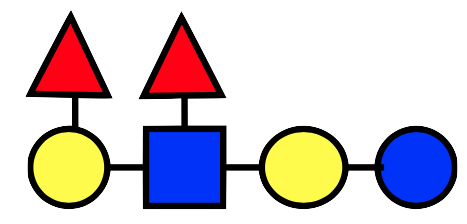
\includegraphics[width=0.7\linewidth, trim={0 -20 0 -20}, clip]{lacto-n-difucohexaose-i.png}} \\[-0.1em]

\rowcolor{white}Asialo galactosylated, fucosylated biantennary &  & 
\vcentralise{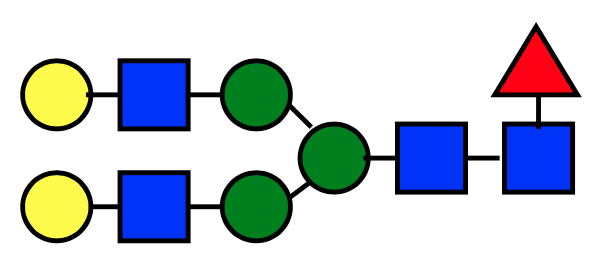
\includegraphics[width=0.8\linewidth, trim={0 -50 0 0}, clip]{na2f.png}} \\
Asialo, galactosylated, biantennary & & 
\vcentralise{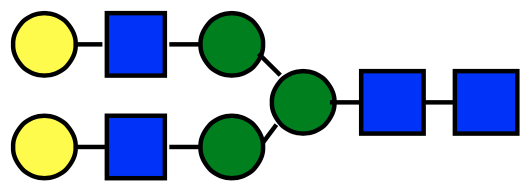
\includegraphics[width=0.8\linewidth, trim={0 -50 0 0}, clip]{na2.png}} \\
Asialo, galactosylated, tetranatennary, N-linked & \multirow{-3}{*}[1.5em]{Complex type N-glycans} & 
\vcentralise{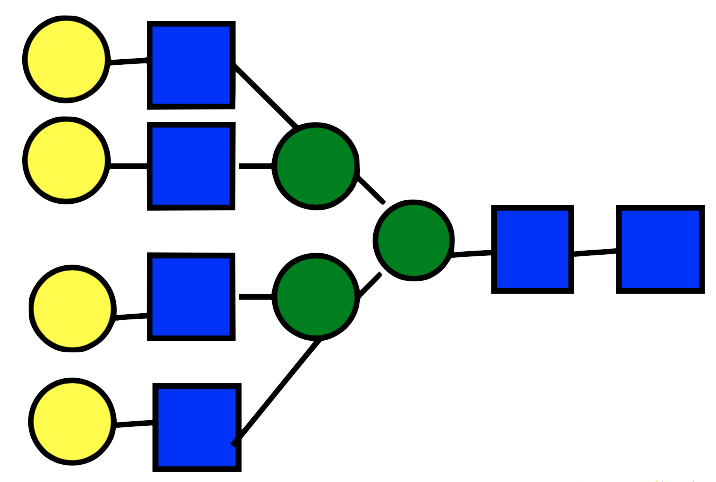
\includegraphics[width=0.8\linewidth, trim={0 -50 0 0}, clip]{na4.png}} \\

\rowcolor{gray!20} $\Delta$UA$\rightarrow$2S-GlucNS & &
\vcentralise{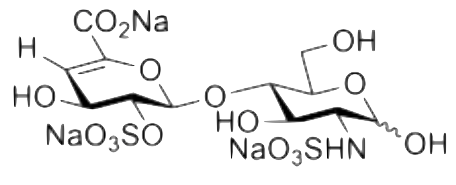
\includegraphics[width=0.9\linewidth, trim={0 -20 0 0}, clip]{2s-glucns.png}} \\
Heparin unsaturated disaccharide I-H & & 
\vcentralise{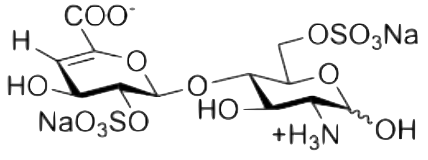
\includegraphics[width=0.9\linewidth, trim={0 -20 0 0}, clip]{hudi-h.png}} \\
Heparin unsaturated disaccharide IV-H & \multirow{-3}{*}[1.4em]{\parbox{\linewidth}{\centering Heparin/Chondrotin derived oligosaccharide}} & 
\vcentralise{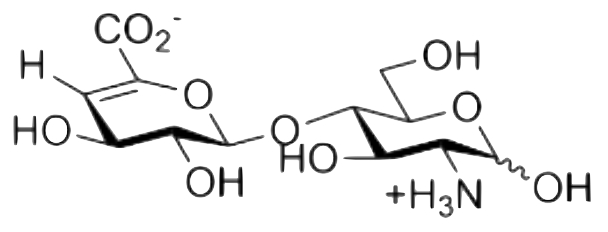
\includegraphics[width=0.9\linewidth, trim={0 -20 0 0}, clip]{hudiv-h.png}} \\

\rowcolor{white}$\alpha$1-6/$\alpha$1-4 mannobiose & oligomannose core structures & 
\vcentralise{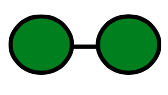
\includegraphics[height=0.9cm, width=1.9cm, trim={0 6 0 6}, clip]{mannobiose.png}} \\

\rowcolor{gray!20}Gal-$\beta$1-6-Gal & Tumour antigens and oligosaccharide core structures & 
\vcentralise{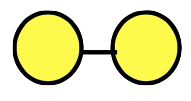
\includegraphics[height=0.9cm, width=1.9cm]{betagal.png}} \\

\rowcolor{white}Gal$\beta$1-3-GalNAc-$\beta$1-4-Gal-$\beta$1-4-Glc &\emph{N}-acetyllactosamine analogues & 
\vcentralise{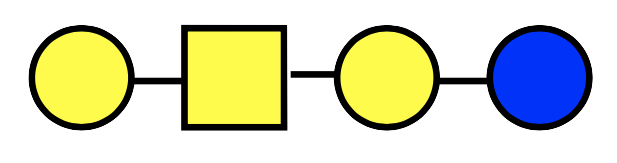
\includegraphics[height=1cm]{galgalnacglc.png}} \\

\rowcolor{gray!20} 3'-sialyllactosamine & & 
\vcentralise{\includegraphics[height=1cm]{3sialyl.png}} \\

LS-tetrasaccharide C (LSTc) & \multirow{-2}{*}{sialylated oligosaccharides} & 
\vcentralise{\includegraphics[height=1cm]{lstc.png}} \\

\rowcolor{white}Neocarratetraose-$4^{1,3}$-di-O-sulphate (Na+) & Neutral and sulfated Galacto-oligosaccharides & 
\vcentralise{\includegraphics[width=0.9\linewidth, trim={0 -10 0 -10}, clip]{neocarratetraose.png}} \\

\hline

\end{tabularx}
\endgroup
\normalsize

\newpage
\section{Discussion}
Tail fibres are an integral part of the mechanism underlying phage life cycles, and more broadly, `free-living' caudate structures. If the literature that suggests `trapped' caudate structures like the T6SS have `antennae' is correct (see \vref{t6ssEMs} and \cite{Chang2017}), it may be the case that tail fibres are an essential part of most if not all caudate structures. At the beginning of this work, various seemingly unusual orthologies for the PVC tail fibres were detected, including assorted phage and Adenoviral fibre motifs. It was unclear whether these were meaningful or spurious since the matches often did not cover the whole protein, the same domains were not always detected between different putative tail fibres, and often had poor similarity statistics. An appealing hypothesis was formed however, namely, that the proteins may represent natural chimeras between `anti-eukaryotic' viral binding moieties (Adenoviral motifs), and more T4 phage-like domains to maintain a mounting interface with the rest of the phage-like tube. If this hypothesis proves correct, these proteins represent, to our knowledge, the first natural example of chimerism between viral sequences of prokaryotic/phage origin, and those of viruses from higher organisms. This chapter set out to shed some of the first experimental light on these proteins, to examine if this split domain architecture and putative similarity to Adenoviridae was valid.

\subsection{Cloning, Purification, and Characterisation of PVC Tail Fibres}
Fortunately, the tail fibres appeared amenable to tagging and purification overall, though PVClumt13 was significantly easier to work with. It was observed that no signal resulted from a C-terminally tagged PVCpnf13 tail fibre Western blot after expression (\vref{pnf13expressiontrial}). The most likely explanation for this is that the C-terminus is buried within that particular structure, so it may be the case that the protein is still expressable but simply not detectable, as it was possible to express PVClumt13 in this manner. In the latter case, reduced yield of protein was also observed, though this could be down to subtle differences in the vector behaviour since the proteins were not in identical backbones, though they were both pET vectors.

Similarly, even between constructs with the same vector backbone, there was a reasonable degree of difference in the amount of protein expressed. PVCpnf13 consistently yielded less protein than did PVClumt13. It's possible that this is simply due to PVCpnf13 being approximately twice the mass/size of PVClumt13, which simply means less protein is synthesisable for the same starting raw materials. Nevertheless, both proteins were able to be purified efficiently with a relatively simple metal ion affinity and gel filtration process, directly from crude cell lysates. Now that it has been devised for these tail fibres, this protocol is already being tested on additional fibres from other PVC operons, and hopefully in future it will aid in unpicking the precise molecular interactions of all of these proteins, which will in turn shed light on the manner in which PVCs are deployed `in the wild'.

It is important to have information about the folded state of any expressed protein. This is particularly so if, as in this study, downstream functional information is desired. Circular dichroism has long been a go-to technique for the cheap and non-destructive structural characterisation of biomolecules, and in particular, proteins. The fact that seemingly intact protein (indicated by its formation of tell-tale trimers (\vref{trimerism})), could be purified was a positive early indication that the tail fibres may be expressing, assembling, and folding correctly, though this by no means guarantees it - probing the secondary structure with CD was therefore a logical step. Reproducible spectra were obtainable from entirely separate protein preparations which  suggests the fold of the proteins is intact and correct, and did not vary from purification to purification. Moreover, analysis of the obtained spectra reveals that the putative PVC tail fibres have a secondary structure profile that is consistent with that seen in a myriad of other tail fibre-like structures (\vref{comparisons}). Not only this, but temperature ramping experiments which were consistent with the observation of limited unfolding in SDS-PAGE assays at elevated temperatures, also agrees with the known thermal stability of tail fibre proteins \citep{Papanikolopoulou2004a, Papanikolopoulou2008, Gazit2008}. One plausible explanation for why the PVCpnf tail fibre is much hardier than the PVClumt fibre could be by its increased length, and therefore repetitiveness. If the repeat motifs are indeed responsible for coordinating metal atoms, it stands to reason that pnf13 will coordinate more than lumt13, potentially conferring much increased stability.

In the dichroism temperature ramping studies, a shift of secondary structure was identifiable for both proteins at approximately 50-55\degC. For PVClumt13, this seemed to largely abolish the secondary structure of the protein, with the signal intensity lessening across the spectrum. For PVCpnf13, an additional secondary structure shift occurs at around 60\degC{}, whereby the spectra actually gains intensity in some areas. The significance of this secondary structure change is unknown, though it likely accounts for the difficulties encountered when attempting to have the pnf13 protein migrate in to SDS-PAGE gels. Two possible speculative explanations for the transitions may include, firstly, that the abrupt shifts in structure correspond to a rapid collapse of the protein. As they are putatively extended, fibrous proteins, this may indicate a collapse of the shaft like regions, and the protein essentially becoming more `globular'. The second hypothesis may be that this is in some way analogous to the proposed conformational changes that occur in phage tail fibres to transduce the binding signal that then trigger contraction. The latter is probably less likely, and what is being seen is simply the denaturing of the proteins, but as this is the limit of the structural resolution of circular dichroism, a concrete answer will have to wait until their structures are fully resolved in future. The (albeit limited) attempts to identify crystallisation conditions (\vref{crystals} and \vref{crystalconditionstable}), are promising however, and resolving the structures of these enigmatic proteins in future may reveal some novel structural patterns.

Structural homologies to phage proteins varied between different fibre proteins, and included hits to the fibritin `whisker' proteins, and both the long and short fibres. Previous elucidations of structural domains for the long tail fibres have shown that they are comprised of multiple proteins - gp34/gp35/gp36/gp37, with gp34 as the proximal phage `mounting hardware' and gp37 at the distal end for receptor recognition. The long tail fibres also require the presence of two additional chaperones, gp38 and gp57 in order to ensure correct structural formation \citep{Granell2014, Bartual2010}. This suggests that the PVC tail fibres are more reminiscent of the short fibres than the long. This may also be consistent with any specificity the PVCs have, since the short fibres of phage are responsible for the `fine' and irreversible binding of the phage to its target cell. The phage gp12 short fibre proteins are also known to require the presence of gp38 to fold \citep{Hashemolhosseini1996}. If it is assumed that the PVC tail fibres are indeed forming correctly, then no such dependence on specific chaperones seems apparent. In the case of the short fibres specifically, \cite{Hashemolhosseini1996} showed that chaperons from phage $\lambda$ (phage Tail fiber assembly proteins (pTfa) could `step in' and ensure correct folding of T-even phage tail fibres. Therefore this is perhaps indicative of PVC tail fibres either being chaperone independent, or simply relying on other endogenous Enterobacterial chaperones such as GroEL, since they could be expressed outside of \emph{Photorhabdus} with no additional proteins, and there are no obvious candidate chaperones within the PVC operons themselves. 

All in all, this provides the first compelling experimental evidence that the putative tail fibres of PVCs do indeed elaborate proteins with many of the hallmarks of known fibre proteins.

\subsection{The Chimeric/split Domain Structure of PVC Tail Fibres}
As explored in \vref{domainstructuresection}, domain structure within the tail fibres appears split, making the PVC tail fibres reminiscent of chimeric phage-Adenovirus `adapters'. Natural phage tail fibres are thought to display some mosaicism with the tail fibres of other, unrelated, phage, meaning that the fibres are essentially recombination hotspots. To date, this recombination appears limited to phage-to-phage recombination, and the exact mechanism is subject to debate \citep{Sandmeler1994}. 

There is literature precedent for a number of artificial phage to eukaryote virus fibre fusions to date \citep{Papanikolopoulou2004a, Papanikolopoulou2004, Krasnykh2001}. Since they all share a similar intertwined ``$\beta$-spiral" trimeric structure (despite not sharing much, if any, sequence similarity), they appear very amenable to these kind of modifications. Fibrous proteins in nature are well studied at this point, with familiar examples such as collagens and amyloid fibrils among the most intensely studied to date. These fibrous proteins are typically made of $\alpha$-helical triple spirals and coiled coils \citep{Beck1998}. Fibres comprised of $\beta$-spirals are comparatively less well studied, but nevertheless widespread, with it being the dominant structure in the fibrous proteins of Adenoviruses, Reoviruses, and phage \citep{Papanikolopoulou2004, Papanikolopoulou2004a}. Thus, any additional examples of fibre proteins which can be better understood structurally will offer insight in to this class of fibrous domain, particularly for putative chimeric proteins, as in artificial studies the exact fusion regions were not well resolved due to their flexibility.

It appears \emph{Photorhabdus} has added to its `biological box of tricks' by seemingly creating such a fusion naturally - or something resembling a fusion; it may be the case that this is an example of convergent evolution, aimed at exploiting the same eukaryotic cell surface markers. The engineering of these fibres, including their artificial fusion, has been an active area of research in order to derive new viral vectors with new tropisms for cell and gene therapies \citep{Krasnykh2001, Li2006}. A particularly interesting example of such a fusion actually appears as a favourable result in the HHPred data shown in \vref{domainstructure}. The top hits for PVClumt13, and the 4th and 5th best hits for PVCpnf13 are all to the PDB ID 1V1H, which is an artificial fusion of the T4 fibritin `foldon' domain, and the globular head of the human Adenovirus 2, created by \cite{Papanikolopoulou2004}. Yet more evidence for the tail fibres correct conformation can be taken from the paper, where the authors note that the chimeras they produced had the characteristic heat, SDS, protease resistance of `normal' fibres.


\subsection{Candidate Binding Targets for PVC Tail Tibres}
The glycan array studies conducted with the PVClumt13 fibre, although still very preliminary, show promise for identifying candidate binding targets. Firstly, it was possible to detect signals, proving that the tail fibres have at least some lectin-like activity. This is consistent with existing studies of bacteriophage and Adenoviral tail fibre-like proteins, whereby glycan arrays have also been used to demonstrate binding (and this is by no means an exhaustive list) \citep{Guardado-Calvo2010, Singh2015, Lenman2018, Nilsson2011}.

The hits obtained from the glycan array appear to be relatively rich in galactose moieties. Phage are known to bind a wide selection of different sugars, of which galactose is one, and has been shown to be used by members of the \emph{Siphoviridae} \citep{BertozziSilva2016}. Another promising indication is the presence of sialylated sugars in the list of results, as silayl sugars are known receptor binding moieties for a number of eukaryotic viruses including Influenza, Rotaviruses, and of particular relevance, Adenoviruses. Numerous previous studies have demonstrated the binding relationships between a number of different Adenovirus species in many different organisms. For instance \cite{Singh2015} have shown that the fibres from the turkey Adenovirus 3 utilise sialylated cell surface markers as their recognition sites. Human Adenovirus 52 requires polysialic acid as its cell surface marker. Both of the sialylated sugars identified for PVClumt13 are adjoined to a galactose residue, and in the case of Adenovirus species D, they have been demonstrated to bind preferentially to this conformation \citep{Burmeister2004}. As a final example, the canine Adenovirus 2 fibres mimic SIGLEC  (Sialic acid-binding immunoglobulin-type lectins) proteins in structure, despite sharing little to no sequence homology, underscoring the potential evolutionary drive to exploit these motifs \citep{Rademacher2012}.

It is thought that these viruses target these types of sugar due to their near ubiquitous appearance and high abundance on eukaryotic cell surfaces \citep{Varki2012}. This does raise questions around tissue specificity for the PVCs however. The variability seen in the tail fibres was initially hypothesised to potentially confer differential targeting against specific cell types, though the use of sialyl sugars would run counter to this. That said, this data only considers a single tail fibre, and it may be the case that other tail fibres are honed in different ways. There may be an evolutionary advantage for \emph{Photorhabdus} to posses a variant of the PVCs which are capable of wide efficacy. The fact that sialic acids are extremely well conserved in the innate immune system across eukaryotic domains of life also goes a long way to explaining the capabilities of \emph{Photorhabdus} virulence factors such as the PVCs in both insect and human infection, since they could plausible retain a mechanism of action with no `additional evolution' required for functionality in a new host.

As mentioned, these results are still preliminary, and will need further replicates to be certain. Additionally, it may be informative to screen other glycan arrays with larger numbers of glycans present (the arrays used here were just over 100 glycans, but arrays are available with in excess of 400 such as that used in the paper by \cite{Guardado-Calvo2010}). This work also needs replicating for the PVCpnf13 tail fibre, and ultimately in future it would be ideal to be able to screen the full library of tail fibres in this manner, to understand the `spectrum' of binding for the natural `library' of fibre proteins. Should the chimeric nature of the tail fibres be borne out in further structural study, there will also be additonal work needed to attempt to unpick whether the glycan specificies detected here reflect the behaviour of Adenovirus-like domains or phage-like domains, since there are some overlaps in the moieties both are able to bind. It seems likely however, particularly with the specificity for sialic acid bearing glycans, that this is the first experimental indication that the tail fibres incorporate a domain that mimics Adenoviral binding mechanisms, as this is one particular glycan type that does not appear to overlap with the binding of phage tails.

This early data also potentially correlates with some of the findings from the proteomic pulldown assays. There are a number of hits which are difficult to reconcile functionally, such as the appearance of the SERPIN protease inhibitor, Dermicidin antimicrobial peptide, and the FAM184A protein which has no known function at present. Lipocalin-1 is known to have an extremely wide binding range with a large number of ligands, likely due to its proposed role in olfaction, and the need to be able to detect many different compounds in the air \citep{Flower1996}. This wide range of binding activity may account for any association with the tail fibres. It may be the case that its enrichment in the presence of the fibres is as a result of `promiscuous' binding, rather than any real meaningful or informative interaction.

However, among the putatively enriched proteins are a number of cell surface associated molecules. Most prominent among these are four protein components of the desmosome (`binding bodies'), a protein complex responsible for cell-cell adhesion, particularly in epithelia \citep{Delva2009}. There is always the possibility of identifying contaminating proteins in proteomic experiments with epithelial proteins being a particular risk (by far the most common of which are keratins). The enrichment of the desmosome proteins relative to controls (as a significant hit), and the fact that desmosome proteins are not listed as primary contaminating proteins in online databases such as the Repository of Adventitous Proteins\footnote{\url{https://www.thegpm.org/crap/index.html}} suggests that these may be meaningful results. Being a cell surface associated protein which is enriched in a cell lysate may be indicative of the kinds of targets which tail fibres will bind to, though the precise mechanism will require much more extensive elucidation. It is possible however that the use of cellular lysates has lead to a spurious result, as the desmosomes, \emph{in vivo}, would likely not be readily accessible when tissues are joined together tightly. One possible explanation consistent with the glycan study however, is that both Desmocollin-1 and Desmoglein both contain N-linked N-Acetyl-Glucosamine and N-linked N-Acetyl-Galactosamine residues respectively \citep{Ramachandran2006}. One final caveat to mention is that the preliminary studies have only been conducted with an epithelial cell type (A549 lung epithelial carcinoma cells), and so it may be due to the cell type assayed that proteins abundant in epithelial cells are identified as significant. One might expect however, that there are numerous proteins enriched in epithelial cells which have not been detected by this assay, and so some specificity of interaction can potentially be inferred.

As discussed in the previous paragraphs, the glycan array results are relatively abundant in both of these moieties, particularly galactose. Similarly, lactotransferrin which was also detected in the pulldown assays contains 3 N-linked N-Acetyl-Galactosamine conjugated residues. Interestingly, lactotransferrin is known to promote the binding of species C Adenoviruses to epithelial cell surfaces, when the Coxsackie-Adenovirus Receptor is not readily accessible \citep{Johansson2007}. It may therefore be plausible that the putatively Adenoviral motifs of the PVC tail fibres are also capable of binding these proteins based on their glycan structure, and may even be exploiting the same mechanism as the Adenoviruses.



\subsection{Summary and Future Work}
As the first experimental studies of these proteins, there is a substantial amount that could be done in future. At the very least, it would be ideal to be able to clone, express, and resolve structures for tail fibres from all of the different PVC operons to better understand the diversity that is so apparent from the results in \vref{bioinformatics}. If these proteins are indeed natural chimeras between phage like tail fibres and Adenoviral fibres, the fact that there are many hypervariable tail fibres in the different operons suggests that the mechanism of `fusing' or evolving new tail fibres is ongoing in various branches of the \emph{Photorhabdus} phylogenetic tree. Thus, not only would this represent the first known example of a natural chimerism for any particular tail fibre, but that there are many natural chimeras, another novel finding in itself.

There are a considerable number of proteins to test, and, as the most physiologically relevant cell/tissue types for PVC activity have yet to be determined, there are a great many more cell types to assay in order to bolster this early data, though some promising leads have been identified already. If the PVCs function on very specific cell types to control the virulence process in intricate ways, it may be the case that very particular cell types will return hits to important markers which will go undetected when testing on just a handful of cell types in the lab. Similarly, it would be ideal to test the tail fibres against much wider arrays of glycans, and of course, simply repeating the studies to be more confident in the binding profiles will be necessary. Based on the work here though, future studies should be made more feasible, as it has been demonstrated that tail fibres from PVCs are amenable to expression without the need for additional chaperones, refolding, or any intricate purification techniques. This should allow the purification of many more of the fibres with techniques ensuring adequate yields for further functional studies.

To begin to answer the tissue specificity and \emph{in vivo}/physiological localisation question an alternative nanoparticle strategy that replaces the iron nanoparticles with gold is currently being developed. Gold nanoparticles exhibit an interesting property in solution, whereby their colour changes due to the phenomenon of having surface plasmons (oscillating electrons in a coherent but delocalised `shell' at the interface between 2 differently charged materials) in a manner dependent on their size or concentration. Concentrated gold nanoparticle solutions are a pinkish-red colour, and the more diluted they are the `blue-er' the solution becomes. This allows accurate concentration estimates based on standard curves from the gold particles as they concentrate/aggregate. This opens up the possibility of quantifying the amount of binding to cell surfaces for instance (in a manner essentially like a `gold-based ELISA'). As gold is not found in natural tissues, the amount of gold present can be quantified very accurately through techniques such as plasma atomic emission spectroscopy. One particularly appealing application of this spectroscopy would be to study localisation in whole animals (insects, for instance) by dissecting out different organs/regions and then quantifying the retained gold

In summary, the results presented in this chapter represent the very first foray in to the experimental investigation of the PVC tail fibres. The state of knowledge prior to this study was entirely based on bioinformatic inferences and the nature of the proteins was far from conclusively understood. To summarise, these results have shown experimental protein similarities to known tail fibre proteins in their trimerism and thermal stability, secondary structure profiles, lack of requirement for dedicated phage-like chaperons, and have begun to shed some light on the functional basis for the putative sequence similarity observed to Adenoviruses, with some compelling, albeit preliminary hits for binding targets.